\documentclass[book,a5paper,12pt,twoside,openany]{memoir}
% Adds the possibility of sensitive hyperlinks in the document itself.
\usepackage{hyperref}
\usepackage{nameref}
\usepackage[utf8x]{inputenc}
\usepackage[english]{babel}
\usepackage{url}
\usepackage{lipsum}
% According to the requirements of IICT-BAS, there should be no page numbering in the manuscript.
%\usepackage{nopageno}
\usepackage{shorttoc}
\usepackage{graphicx}
% Directory where the images are located.
\graphicspath{{images/}}
\usepackage{array}
\usepackage{imakeidx}
\usepackage{placeins}
\usepackage{titling}

% Title of the book.
\title{Scientific Computing with\\Java and Android\\-\\Practical Guide}

% Names of authors.
\author{Todor Balabanov, Iliyan Zankinski, Petar Tomov}

% Automatically create an alphabetical index.
\makeindex[columns=1, title=Index, intoc]

\begin{document}

\maketitle

% The title page does not match the layout of the rest of the document (no numbering).
\thispagestyle{empty}

\newpage

Scientific Computing with Java and Android

Practical Guide

by

Todor Balabanov, Iliyan Zankinski, Petar Tomov

\vspace{0.4cm}

Independently published by

Kindle Direct Publishing

\vspace{0.4cm}

Velbazhd Software LLC

Mladost 1, 18, 5, 6, 16, 1750 Sofia, Bulgaria

\vspace{0.4cm}

https://www.veldsoft.eu/

\vspace{0.4cm}

Copyright © 2022,

Todor Balabanov, Iliyan Zankinski, Petar Tomov

\vspace{0.4cm}

All rights reserved. No portion of this book may be reproduced in any form without permission from the publisher, except as permitted by U.S. copyright law. For permissions contact: velbazhd.software@gmail.com +359 89 8237103

\vspace{0.4cm}

ISBN: 0000000000000 (print)

Printed by request

1st Edition

\newpage
\addcontentsline{toc}{chapter}{Acknowledgments}
\chapter*{Acknowledgments}

This work is supported by the Bulgarian National Science Fund by the project - Mathematical Models, Methods, and Algorithms for Solving Hard Optimization Problems To Achieve High Security in Communications and Better Economic Sustainability, Grant Number: KP-06-N52/7.


% Here is the table of contents generated from the chapters' titles.
\newpage
\shorttoc{Topics}{0}

% Here is the table of contents, which is generated from the title of the chapters and the title of the sections.
\newpage
\tableofcontents

% Thus, the numbering of the subpoints is in Arabic numerals.
\renewcommand\thesection{\thechapter.\arabic{section}}
\renewcommand\thesubsection{\thesection.\arabic{subsection}}

\newpage
\addcontentsline{toc}{chapter}{Предговор}
\chapter*{Предговор}

Това учебно помагало е предназначено за ученици и студенти, които биха искали да се запознаят с възможностите за реализиране на изчисления в разпределена среда\index{изчисления в разпределена среда} с използването на програмния език Java и мобилната платформа Android.

В съвременното ни ежедневие ние все по-често сме заобиколени от мобилни изчислителни устройства. Най-често това са мобилни телефони, таблети, часовници или други форми на wearables (миниатюрна електроника под формата на модни аксесоари или части от дрехи). До преди десетилетие този вид мобилни устройства бяха рядкост, а изчислителните им възможности бяха изключително ограничени. Тези два факта не позволяваха мобилните устройства да бъдат използвани за нещо повече освен основния принцип на употреба за който са създадени. С развитието на микроелектрониката и миниатюризацията на компонентите, съставящи мобилните устройства, техните възможности значително нараснаха за последното десетилетие. Това позволява върху този вид устройства да се извършват и допълнителни задачи, които не са били предвидени при първоначалното им проектиране. Паралелно с развитието на мобилните технологии бурен подем претърпяха и възможностите за мобилна комуникация като GSM, 3G, 4G, Wi-Fi, Bluetooth, NFC и други. Комбинацията между относително мощни мобилни изчислителни устройства и добре развита комуникационна среда открива безгранични възможности за приложение на мобилните устройства при извършването на допълнителни изчисления в разпределена среда\index{изчисления в разпределена среда}. 

В настоящето учебно помагало  запознаваме читателите с интересните възможности, които предлагат съвременните Android мобилни устройства\index{мобилни устройства}, за постигането на резултати в научни изчислителни задачи, разпределяйки изчисленията върху физически отдалечени едно от друго устройства. Изложението на материала е организирано в следните глави. 

Глава 1 - \nameref{chapter01}: Дава кратко описание на идеята за научни изследвания и по какъв начин те могат да се впишат в ежедневния живот и използването на „умни“ мобилни устройства.

Глава 2 - \nameref{chapter02}: Представят се някои от популярните евристични подходи за решаване на сложни изчислителни задачи. Обяснява се и разликата между точните числени методи и приближените изчисления. По-сериозно внимание се отделя на генетичните алгоритми и изкуствените невронни мрежи, тъй като те са в основата на разработваната система. 

Глава 3 - \nameref{chapter03}: Излагат се различни аргументи за изготвянето на една софтуерна архитектура и се дават насоки за реалната разработка на един софтуерен проект. Изборът за архитектура на системата е насочен към трислойните модели, както в контекста на системата клиент-сървър, така и в контекста на локално мобилно приложение, което се състои от потребителски интерфейс, работна логика и локална база данни. 

Глава 4 - \nameref{chapter04}: Детайлно се представя процесът по създаването на едно мобилно приложение, което има за основна задача извършване на изчисления във фонов режим чрез използване на възможностите, които  операционната система Android дава. Това включва приложение за активен тапет, екран за настройки и група класове за вътрешно представяне на информацията. 

Глава 5 - \nameref{chapter05}: Показва реализацията на отдалечената част от системата, а именно уеб базиран сървър с релационна база данни. За съхраняването на суровата информация за валутните котировки и параметрите на изкуствените невронни мрежи е представено MySQL базирано решение под формата на релационна база данни. За обмен на информацията между отдалечената база данни и мобилните приложения е представено PHP базирано решение. 

Глава 6 - \nameref{chapter06}: Набляга на комуникацията между отдалечения сървър и локалните клиенти, изпълнявани върху мобилни устройства. Тъй като от страната на сървъра е избрано уеб базирано решение, то в основата на комуникацията е заложен HTTP протоколът и неговите възможности да предава JSON пакетирани съобщения. 

Глава 7 - \nameref{chapter07}: Разглежда обучението на изкуствени невронни мрежи, което е свързано с намиране на такива оптимални стойности за теглата, че мрежата максимално добре да изпълнява задачата, за която е предназначена. При липсата на обратни връзки се използва обратно разпространение на грешката, а при наличието на обратни връзки генетични алгоритми. 
\newpage
\chapter{Научни изчисления}
\label{chapter01}

Още в зората на съвременната изчислителна техника най-съществените пресмятания са били с научна насоченост и военно дело. Този факт не се е променил значително за последните десетилетия. Дори в наши дни най-сериозните изчислителни ресурси са насочени в областта на науката. Това дава основание да обърнем значително внимание на начините, по които можем да изпълняваме научни изчисления дори и върху изчислителни устройства, чието основно предназначение не е с научна цел. 

\section{Последователно програмиране}

При последователното програмиране\index{последователното програмиране} всяка изчислителна инструкция следва всички предходни. В зората на изчислителната техника пресмятанията са извършвани по този начин. Дори в наши дни значителна част от алгоритмите се изпълняват само последователно, тъй като входните данни за всяка инструкция зависят от изходните данни на предходните инструкции. Последователните алгоритми не подлежат на декомпозиране и поради тази причина са неприложими за паралелни пресмятания (Фиг. \ref{fig:pic0001}). 

\begin{figure}[h]
  \centering
  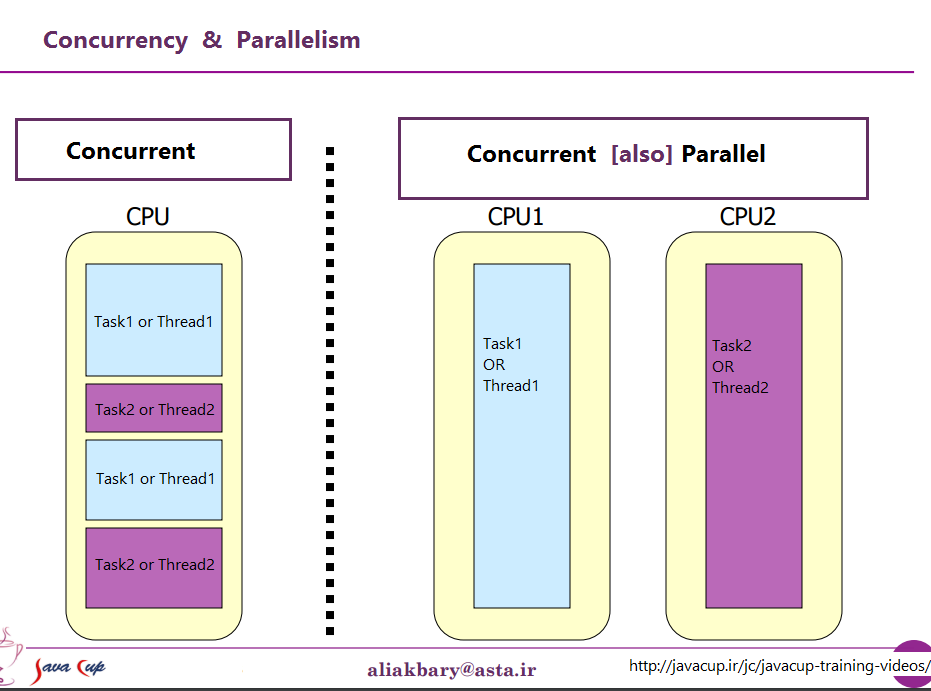
\includegraphics[width=1.0\linewidth]{pic0001}
  \caption{Сравнение между последователни пресмятания и паралелни пресмятания}
\label{fig:pic0001}
\end{figure}

\section{Паралелно програмиране}

При паралелното програмиране основно се говори за две разновидности - конкурентни пресмятания\index{конкурентни пресмятания} и паралелни пресмятания\index{паралелни пресмятания}. Конкурентните пресмятания са в среда, където група от задачи могат да се пресметнат едновременно без да има значение от реда на пресмятане. В същото време, паралелните пресмятания се отнасят за едновременно пресмятане на отделни задачи върху отделни процесори. В този контекст всички паралелни пресмятания са конкурентни пресмятания, но не и обратното (Фиг. \ref{fig:pic0002}). 

\begin{figure}[h]
  \centering
  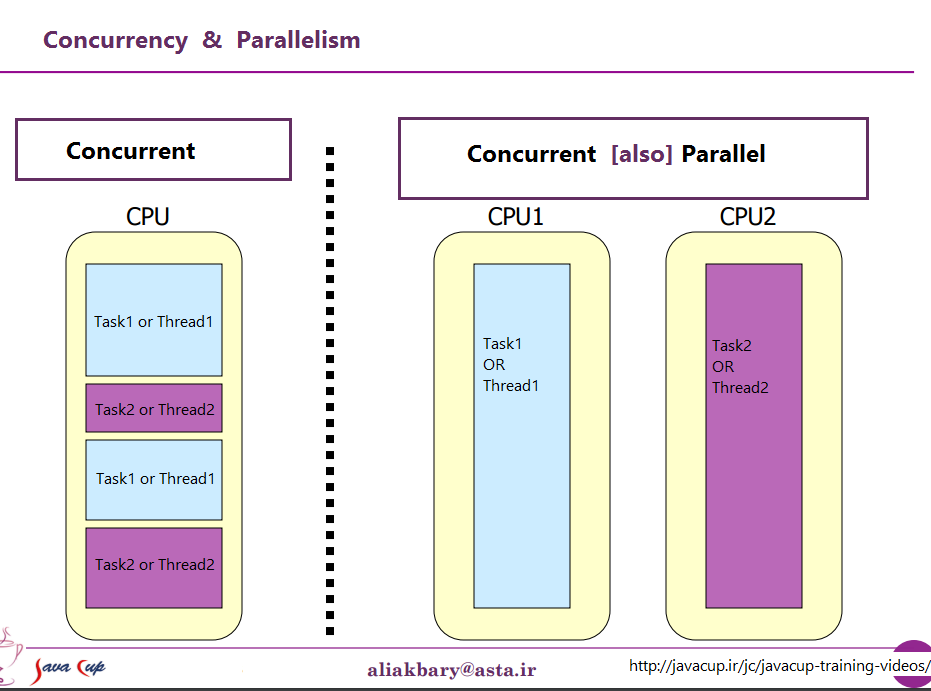
\includegraphics[width=1.0\linewidth]{pic0002}
  \caption{Сравнение между конкуретни пресмятания и паралелни пресмятания}
\label{fig:pic0002}
\end{figure}

\section{Супер компютри и грид изчисления}

Когато паралелните алгоритми се изпълняват на изчислителни машини с множество процесори и/или множество ядра на процесорите, този вид изчисления се определят като супер компютърни\index{супер компютърни изчисления} (supercomputing). Същественото при този вид пресмятания е, че се използва много бърза вътрешна шина (понякога оптична) и споделена оперативна памет. За разлика от супер компютрите\index{супер компютърни изчисления}, грид изчисленията\index{грид изчисленията} се осъществяват на множество машини свързани в обща мрежа, но работещи автономно без да споделят обща памет. При грид системите отделните изчислителни машини могат да са териториално отдалечени една от друга. Съществено е да се отбележи, че и при супер компютрите\index{супер компютърни изчисления} собственикът на системата има пълен контрол над нея. Това може малко да се различава за грид системите, ако към грида са включени компютри под чужд контрол. 

\section{Изчисления в разпределена среда}

Преходът от грид системите към системи за изчисления в разпределена среда\index{изчисления в разпределена среда} се състои в това, че изчислителните машини в разпределената среда са абсолютно автономни. Тези машини не споделят общи ресурси като процесор или оперативна памет. Много характерно е в разпределената среда контролът над изчислителните машини да не е от страната на организиращия изчисленията. Това води до два основни проблема - ненадеждна (често и твърде бавна) комуникация, липса на гаранция за коректност на пресмятанията (манипулации от страна на притежаващия изчислителните ресурси). Също така, при грид системите често се наблюдава хомогенност на изчислителните ресурси по отношение на хардуерни конфигурации и операционна система, докато в разпределената среда изчислителните машини са основно хетерогенни, което може да води до големи разлики в хардуера и операционните системи. 

\section{Дарена изчислителна мощност}

За решаването на някои по-мащабни научни проблеми изчислителната мощност и/или финансовите ресурси често са недостатъчни. В такива ситуации не малко научни институции прибягват до така наречените дарени изчислителни ресурси\index{дарени изчислителни ресурси} в разпределена среда\index{изчисления в разпределена среда}. Един от най-изчерпателните списъци с проекти от този вид може да бъде открит в уеб сайта Distributed Computing Info \cite{dcinfo}. Съществено е да се отбележи, че не всеки изчислителен проблем е подходящ за решаване в разпределена среда\index{изчисления в разпределена среда} с дарена изчислителна мощ. На първо място проблемът трябва да подлежи на декомпозиране, така че отделни части от него да се пресмятат едновременно. Второто важно нещо е да не е от съществено значение в кой момент от времето и в какъв ред ще бъдат получени пресметнатите резултати. И третото съществено нещо е да е наличен механизъм за проверка на достоверността от пресмятанията, тъй като изчисленията се извършват на машини с различна хардуерна конфигурация и различни операционни системи, а освен това са възможни манипулации от страна на хората притежаващи тези машини. Най-известният проект за дарена изчислителна мощ е SETI@home \cite{shuch} като неговата цел е да търси сигнали от космоса, които да са създадени от интелигентни форми на живот.

Когато изчисленията се извършват на мобилни устройства, то разпределената среда се превръща в мобилна среда за разпределени изчисления\index{мобилна среда за разпределени изчисления}. В останалата част от това учебно помагало ще бъде представено точно изграждането на система за извършване на разпределени изчисления върху мобилни устройства. 

\newpage
\chapter{Евристични алгоритми}
\label{chapter02}

Евристичните алгоритми са подход за решаване на изчислителни проблеми, основаващи се на опита и интуицията. Този вид алгоритми не гарантират оптимално решение за поставената задача. Евристичните алгоритми намират широко приложение при задачи, които трудно се поддават на точни числени методи или аналитични решения. Макар и да не могат да предложат оптимално решение, евристичните алгоритми\index{евристични алгоритми} често водят до достатъчно приемливи в практиката, близки до оптималното решения. Благодарение на своята не детерминистична природа, евристичните алгоритми\index{евристични алгоритми} са изключително подходящи за реализация в супер компютърни изчисления\index{супер компютърни изчисления}. Две изключително популярни евристики\index{евристики} са изкуствените невронни мрежи\index{изкуствени невронни мрежи} и генетичните алгоритми\index{генетични алгоритми}. Те са обект на особена популярност през последните две десетилетия и това дава основание да бъдат заложени в основното изложение на настоящото учебно помагало. Сами по себе си евристиките са безполезни, ако не бъдат приложени върху достатъчно сложна изчислителна задача. Точно такава сложност предлагат задачите за прогнозиране. Прогнозирането е залегнало в множество дейности от човешкото ежедневие, като започнем от средните дневни температури и стигнем до потреблението на определени стоки и услуги. Под една или друга форма почти всяка човешка дейност бива остойностена в термините на финансовите ресурси. Този факт дава основание да бъдат разгледани точно прогнози за промяната в цените на различни финансови инструменти. Отчитането на промяната в цената, на определени интервали (равни или неравни), води до представяне на информацията във времеви ред\index{времеви редове}. При времевите редове\index{времеви редове} по абсцисната ос се означава времето, а по ординатната ос стойността на измерваната величина (в конкретния случай цената).

\section{Финансови времеви редове}

Времевите редове\index{времеви редове} са серия от замервания извършени в последователен ред във времето. Практически се получава последователност от дискретни стойности. Времевите редове могат да са съставени от стойности на равни интервали или стойности на произволни интервали. Често в практиката се случва да има липсващи замервания, което води до определени усложнения при анализирането. При финансовите времеви редове основно се използват равни интервали на отчитане и рядко има липсващи стойности при отчитането. Всяко едно отчитане при финансовите времеви редове се отличава с група стойности, характеризиращи времевия интервал за който се отнася, а именно – начална стойност за интервала, най-висока постигната стойност за интервала, най-ниска стойност постигната за интервала и крайна стройност за интервала. 

\begin{figure}[h]
  \centering
  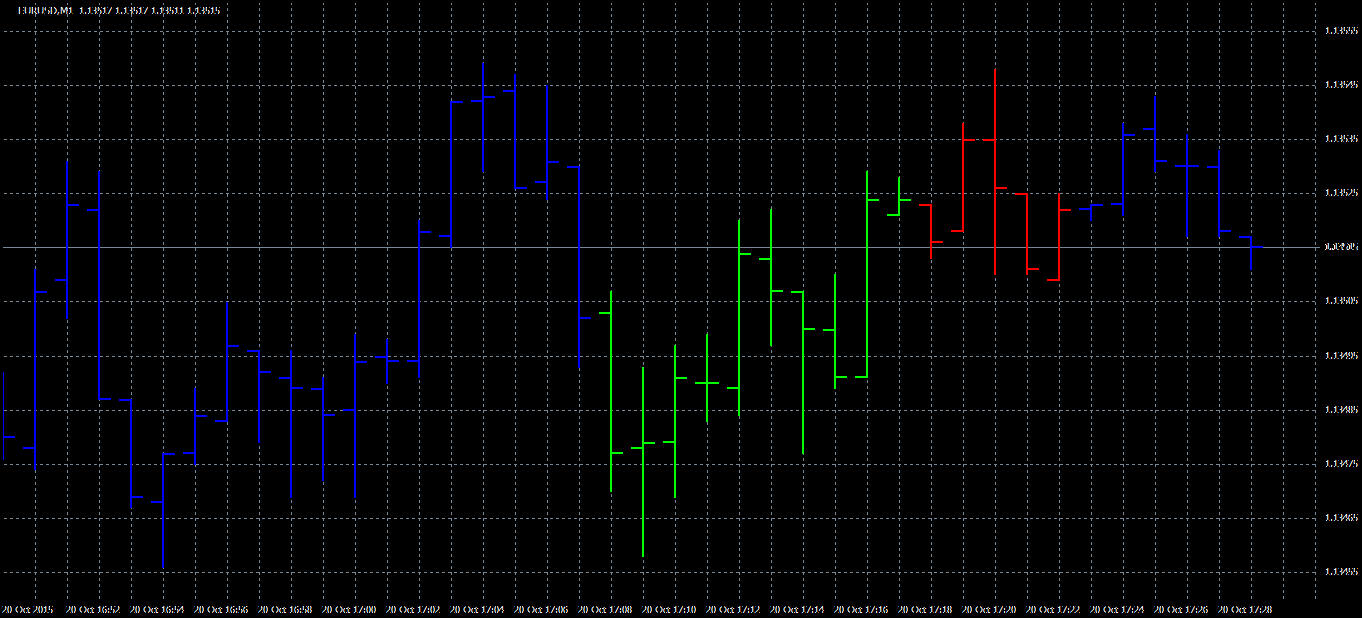
\includegraphics[width=1.0\linewidth]{pic0003}
  \caption{Отношението евро/долар в рамките на един час.}
\label{fig:pic0003}
\end{figure}

На Фиг. \ref{fig:pic0003} тази информация се обозначава с вертикални черти, като долният край на вертикалната черта символизира най-ниското ниво, горният край най-високото ниво, а двете странични чертички маркират нивото на отваряне (отляво) и нивото на затваряне (от дясно). Анализирането на времевите редове\index{времеви редове} може да предостави съществена информация за лицата вземащи решения. Когато става въпрос за времеви редове във финансовата област основна цел на анализа е предлагането на прогноза. Една от най-често използваните форми на анализ е напасването на крива (curve fitting). От математическа гледна точка задачата представлява построяване на крива която да премине максимално близо до предварително определени точки. От математиката е добре известно, че през краен брой точки могат да се построят безкрайно на брой преминаващи криви. За да има смисъл от напасването кривата трябва да притежава определени свойства, като изглаждане, добра интерполация и екстраполация. 

Условното разделяне на финансовия времеви ред\index{финансови времеви редове} на две половини (минало и бъдеще) дава изключително добра възможност за представяне на задачата по прогнозиране в термините на изкуствените невронни мрежи\index{изкуствени невронни мрежи}. Мащабираната информация от миналия период (зелено на графиката) се подава към входния слой на изкуствената невронна мрежа, а прогнозата се получава в изходния слой на изкуствената невронна мрежа и се подлага да обратно мащабиране (червеното на графиката). Така декомпозиран времевият ред\index{времеви редове} се използва при фазата за обучение на изкуствената невронна мрежа. За работната фаза на мрежата за прогноза на изкуствената невронна мрежа се подават последните измерени стойности, без да има яснота какви са бъдещите измервания. 

\section{Изкуствени невронни мрежи}

Изкуствените невронни мрежи\index{изкуствени невронни мрежи} са се появили в следствие на опитите за изграждане на математически модел за биологичните нервни системи. Този вид системи се научават (прогресивно подобряват възможностите си) с изследването на примерни данни. Приложението им е основно при задачи за които традиционните алгоритми не дават приемливи резултати. Най-широко приложение изкуствените невронни мрежи намират в задачи за класификация. Когато става въпрос за финансови времеви редове са възможни две събития – повишаване на стойността или понижаване на стойността. Според информацията в отминалите периоди време, изкуствената невронна мрежа\index{изкуствени невронни мрежи} може да раздели данните в два основни класа – данни показващи промяна към повишение или данни показващи промяна към понижение. 

\begin{figure}[h]
  \centering
  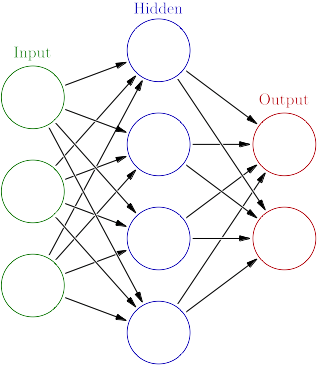
\includegraphics[height=0.25\pdfpageheight]{pic0004}
  \caption{Трислойна изкуствена невронна мрежа.}
\label{fig:pic0004}
\end{figure}

Структурата на класическите изкуствени невронни мрежи\index{изкуствени невронни мрежи} се състои от възли, наречени изкуствени неврони и връзки, наречени тегла (Фиг. \ref{fig:pic0004}). Връзките между невроните служат за предаване на сигнал от един неврон към друг. Невроните които получават сигнали ги обработват по предварително заложено правило и след това могат на свой ред да ги разпространят към други неврони. В класическият случай невроните имат стойност (обикновено това е реално число). Връзките между невроните също са представени със стойност и според правилото за обучение точно тази стойност подлежи на промяна, така че мрежата да заучава необходимата информация. При най-използваните изкуствени невронни мрежи\index{изкуствени невронни мрежи} невроните са организирани в слоеве. Сигналите при този вид мрежи се разпространяват от входния слой към изходния слой, като преминават междинните слоеве. Това разпространение на сигналите се нарича пас в права посока и е характерно за режима на експлоатация. Освен режим на употреба изкуствените невронни мрежи\index{изкуствени невронни мрежи} работят и във втори режим, наречен режим на обучение. За последните няколко десетилетия са предложени множество начини за обучение на изкуствени невронни мрежи, като най-значими резултати се получават при използването на алгоритъма за обратно разпространение на грешката\index{обратно разпространение на грешката}. Обратното разпространение на грешката представлява точен числен метод от групата на градиентните методи, който разчита на грешката, която мрежата допуска при изпълнението на обучаващите примери. Тази допусната грешка се установява в изходния слой и след това се разпространява обратно по предходните слоеве, от където идва и названието на метода. 

Според своята линейна природа, обратното разпространение на грешката\index{обратно разпространение на грешката} трудно се поддава на реализация в термините на паралелното програмиране. Ако се погледне на теглата в една изкуствена невронна мрежа като на многомерно безкрайно пространство от реални числа, то намирането на стойности за теглата е математическа оптимизационна задача. Точните числени методи дават добри резултати при пространства с относително малка размерност, но срещат сериозни затруднения при по-големите размерности. Точно противоположно на точните числени методи, евристичните алгоритми предлагат приемливи решения, в разумно време. Предимство е не само ефективността, но и значително по-големите възможности евристичните алгоритми да се реализират в термините на паралелното програмиране. 

Класическите неврони реализират трансферна функция и активационна функция. Най-често използваната трансферна функция е линейната, която представлява сума от умножение на входните сигнали по теглата, които ги доставят. Най-често използваните активационни функции са сигмоидната функция и хиперболичния тангенс. Активационната функция има основна роля за нормиране на изходния сигнал. Тази нормализация е необходима тъй като за трансферната функция, при различните неврони, постъпват различен брой сигнали и без нормализация това би направило изходните сигнали несъизмерими. При градиентните точни числени методи има изискване активационната функция да бъде диференцируема, нещо което не е необходимо при евристичните алгоритми. Често използваната линейна трансферна функция има нужда от използване на допълнително събираемо наречено „отместване“ (bias). От формална гледна точка, отместването може да се интерпретира като тегло свързващо неврона с друг неврон, който емитира единичен сигнал. В практиката за всеки слой е прието да се отделя неврон емитиращ единичен сигнал. Само в изходния слой е безсмислено такъв неврон да има, тъй като той не получава входни сигнали, а емитирането на постоянна единица в изхода не носи смислена информация за функционирането на мрежата. 

От математическа гледна точка класическите невронни мрежи могат да се представят с вектор (стойностите на невроните) и матрица (стойностите на теглата между невроните). Разпространението на сигналите от входа към изхода в този случай би бил умножение на вектор с число. В настоящото учебно помагало на класическа трислойна мрежа ще се подават мащабираните стойности от изминалите времеви периоди, а на изхода ще се очаква прогнозна стойност за бъдещи времеви интервали. Тази концепция е малко по-сложна от идеята за проста квалификация от вида повишение/понижение, но е значително по-информативна, защото се очаква да дава представа за един по-дълъг времеви интервал в бъдещето. След успешно прогнозиране в коя посока ще се промени цената от съществено значение става и въпросът колко дълго ще продължи този спад/повишение. 

\section{Генетични алгоритми}

Генетичните алгоритми представляват глобална оптимизационна евристика\index{глобална оптимизационна евристика} вдъхновена от идеите за биологичната еволюция. Генетичните алгоритми са подмножество на класовете популационни алгоритми и еволюционни алгоритми. Основното си приложение генетичните алгоритми\index{генетични алгоритми} намират при задачи с голяма по размерност пространство на решенията. Често при такива задачи класическите точни числени методи не могат да предложат решение в приемливо време. За да се приложи генетичен алгоритъм решението на съответната задача трябва да се представи под формата на хромозома (индивид) в обща популация от решения. След това, чрез прилагане на основните операции по селекция\index{селекция в генетичен алгоритъм}, кръстосване\index{кръстосване в генетичен алгоритъм} и мутация\index{мутация в генетичен алгоритъм} (Фиг. \ref{fig:pic0005}), отделните индивиди (решения) следва да бъдат подобрявани.

\begin{figure}[h]
  \centering
  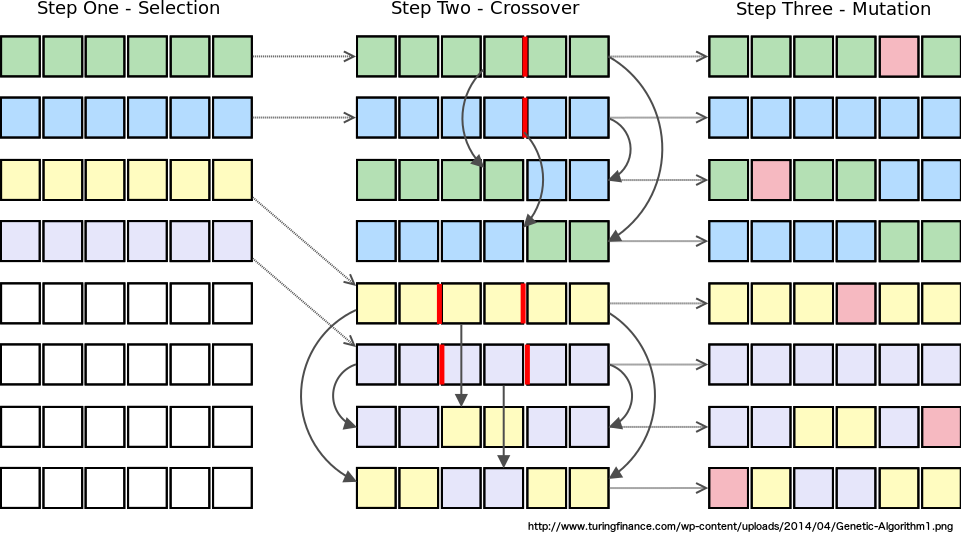
\includegraphics[width=1.0\linewidth]{pic0005}
  \caption{Трите основни операции в генетичните алгоритми.}
\label{fig:pic0005}
\end{figure}

При класическия процес оптимизацията започва от случайно генерирани индивиди, Това не е задължително особено когато става въпрос за хибридни реализации в които генетичният алгоритъм е поддържаща оптимизация. При такива ситуации началната популация може да бъде получена в резултат на друга оптимизация или в резултат на човешка подредба. След началната фаза оптимизацията протича итеративно и приключва според предварително определени критерии за край. Най-често се използва предварително дефиниран брой поколения или брой поколения които не водят до подобрение в намерените решения, но също така е възможно да се дефинира и интервал астрономическо време. 

От основна важност за успешната работа с генетичните алгоритми\index{генетични алгоритми} е определянето на целева функция (жизнена функция\index{жизнена функция} на индивида) която еднозначно да определя качеството на полученото решение. На база различната жизненост която индивидите в популацията притежават се взема стохастично решение кои индивиди да участват в създаването на бъдещото поколение и кои не. В множество реализации на генетични алгоритми се прилага правило на елита, така че най-доброто открито решение да достигне края на оптимизационния процес. В същото време правилото на елита крие риск от израждане на популацията, така че всичките решения в нея да клонят към съхранения елит.  

Фактът, че генетичните алгоритми са организирани на принципа на популацията от индивиди ясно подсказва идеалната възможност оптимизационния процес да се организира не в една глобална популация, а в множество различни локални популации които да съществуват на различни изчислителни машини. Това от своя страна би дало възможност за реализиране на миграционни процеси, точно както това се наблюдава при естествените биологични видове. 

\section{Прогнозиране в разпределена среда}

Гъвкавите възможности на изкуствените невронни мрежи\index{изкуствени невронни мрежи} да изграждат функционална зависимост между входни и изходни данни ги прави идеален кандидат за прогнозираща система. Ако се приеме, че измерените стойности във времевия ред са точки в двуизмерно пространство, то задачата за прогнозиране може да се представи като задача за прекарване на крива през N точки (curve fitting). Ако образно се оприличи изкуствената невронна мрежа на полином, то теглата й биха представлявали коефициенти в полинома. Стойностите които изкуствената невронна мрежа\index{изкуствени невронни мрежи} генерира на изхода си за бъдещи моменти от времето представляват своеобразна екстраполация\index{екстраполация} според апроксимираната крива. Тъй като класическите многослойни невронни мрежи работят с входни сигнали между 0.0 и 1.0 или -1.0 и +1.0, то информацията от времевия ред трябва да бъде мащабирана в съответния работен интервал на мрежата. Стойностите на времевия ред условно се разделят на минали (зелените Фиг. \ref{fig:pic0003}) и бъдещи (червените Фиг. \ref{fig:pic0003}). Изходната (прогнозна) информация на изкуствената невронна мрежа след това се мащабира обратно към оригиналните интервали на времевия ред.

\begin{figure}[h]
  \centering
  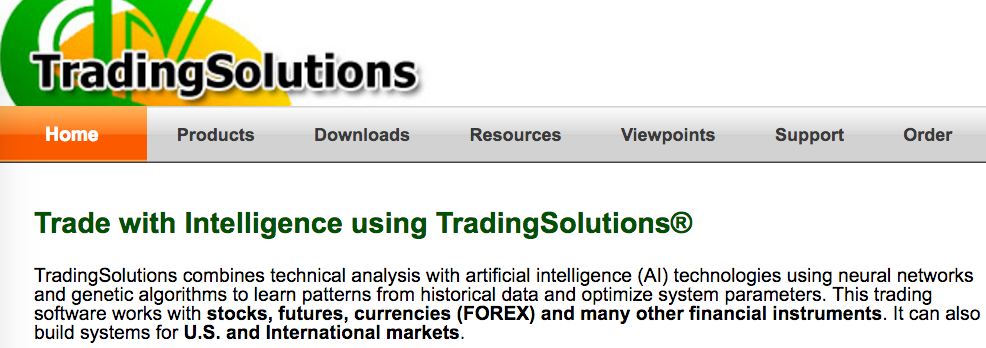
\includegraphics[width=1.0\linewidth]{pic0006}
  \caption{Продуктовата линия TradingSolutions използваща изкуствени невронни мрежи и генетични алгоритми за прогнозиране на Forex финансови инструменти.}
\label{fig:pic0006}
\end{figure}

От чисто практическа гледна точка, използването на изкуствени невронни мрежи и генетични алгоритми се е доказало като удачен подхода за прогнозиране на финансови инструменти, което ясно се вижда в продуктовата линия на TradingSolutions (Фиг. \ref{fig:pic0006}). Почти петнадесет години продуктовата линия на TradingSolutions доставяше системи за подпомагане вземането на решения\index{системи за подпомагане вземането на решения}. По настояще тази продуктова линия е придобита от компанията nDimensional, Inc.

\begin{figure}[h]
  \centering
  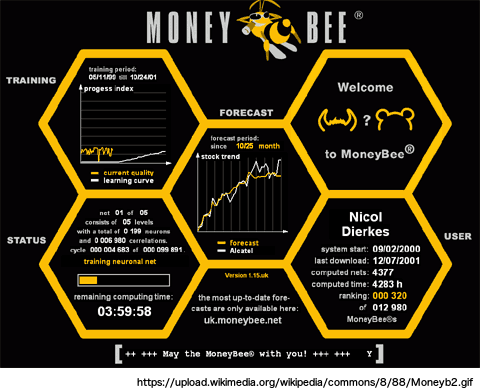
\includegraphics[height=0.4\pdfpageheight]{pic0007}
  \caption{Системата MoneyBee за финансово прогнозиране в разпределена среда.}
\label{fig:pic0007}
\end{figure}

Възможността да се прогнозират цените на финансови инструменти винаги е привличала не само индустрията, но и научните среди. Едно от най-забележителните постижения в тази насока е проектът MoneyBee (Фиг. \ref{fig:pic0007}). Макар и вече да не съществува, този проект предлагаше възможност за изчисляване на прогнози с помощта на дарена изчислителна мощност\index{дарени изчислителни ресурси} в разпределена среда\index{изчисления в разпределена среда} \cite{bohn}. Същинските прогнози се пресмятаха, с помощта на изкуствени невронни мрежи, върху изчислителните машини на потребителите в периоди когато натоварването на машините е ниско и се активира програмата за защита на монитора (screensaver). Преди масовото навлизане на мобилните устройства честа практика при проектите за дарена изчислителна мощност, с цел пресмятане в разпределена среда\index{изчисления в разпределена среда}, основен подход бе извършване на пресмятанията в специално създадена за целта програма за предпазване на монитора. След навлизането на катодно лъчевите тръби при настолните компютри се появява ефект от увреждане на монитора, ако върху него продължително се визуализира статична картина. Решаването на този проблем се оказва най-удачно с помощта на операционната система, която да установи период в който потребителя не използва изчислителната машина и да активира софтуерна програма за предпазване на монитора. Развитието на мониторите с течни кристали постепенно изведе от употреба мониторите с катодно-лъчеви тръби и използването на програми за предпазване на монитора изгуби своето първоначално предназначение. Въпреки това този вид софтуерни решения останаха в употреба и основно служат за повишаване на информационната сигурност, като не само дават естетическа визуализация, но и привеждат работната сесия на потребителя в заключено състояние, което възпрепятства използването на компютърната система от неауторизирани потребители. Наличието на изчислителни ресурси, които са налични, но неефективно използвани дава основание на множество учени да разработят системи за отдалечено пресмятане в разпределена среда\index{изчисления в разпределена среда}, точно под формата на програми за предпазване на монитора, които да се възползват от дарените потребителски, изчислителни ресурси. 

\section{Фонови пресмятания върху мобилни устройства}

Съществува концептуална разлика в начина по който потребителите използват настолните си компютри и мобилните устройства. На първо място, настолният компютър бива пускан и спиран според нуждите на потребителя, докато най-често мобилните устройства са в непрекъснат режим на употреба. Това води до основната разлика, че мобилните устройства не изпадат в режим на занижена употреба, но също така имат режими за употреба при изключителна важност (примерно телефонно обаждане с висок приоритет). Втората фундаментална разлика се състои във факта, че основен похват за пестене на електрическа енергия, доставяна предимно от батерии при мобилните устройства, е динамичното изгасяне на екрана. Тази стратегия за пестене на енергия кардинално отменя концепцията за програма предпазваща монитора. За да се реализира ефективно система за разпределени пресмятания върху мобилни устройства е много по-удачно да се използва технологията за активен тапет, отколкото да се залага да идеята за програма предпазваща монитора. Точно тази идея е развита в настоящото учебно помагало.
\newpage
\chapter{Софтуерна архитектура}
\label{chapter03}

Разработката на софтуер е в областта на инженерните науки, тъй като продуктът се създава по принципите за изграждане на конструкции (в случая софтуерни). При стартирането на нов софтуерен проект трябва да се вземат редица решения, според заданието на потребителя. В настоящата разработка целта е софтуерно решение което извършва изчисления от страната на клиентски мобилни устройства. Задачите за пресмятане се възлагат от сървър и получените пресметнати резултати се получават обратно на същата машина. От страната на клиента се получават стойности за цена на валути под формата на времеви ред. Сървърът изпраща на клиента също информацията за топология на изкуствена невронна мрежа. Клиента от своя страна използва котировките на валутите и информацията за изкуствената невронна мрежа за да извършва пресмятанията необходими за обучението на изкуствената невронна мрежа. Процесът по обучението на изкуствената неверонна мрежа\index{изкуствени невронни мрежи} се извършва с помощта на генетични алгоритми\index{генетични алгоритми}, които имат за цел търсене на възможно по-оптимални стойности за теглата на мрежата. Клиентското приложение също поема отговорностите за визуализация на процеса по обучение и визуализация на постигнатите прогнози. Така представена системата съвсем естествено води към избора на „клиент-сървър“ софтуерна архитектура. 

\section{Избор на развойни средства}

В съвременната софтуерна индустрия има голям избор от развойни средства\index{развойни средства} за различните нужди на софтуерните разработчици. Една част от развойните средства са комерсиални, докато друга част са инструменти с отворен код. В настоящата разработка акцентът основно пада върху развойни средства с отворен код, тъй като минимизирането на разходите за производство е основен стремеж с цел постигане на икономическа ефективност. Изборът на развойни инструменти е задача от областта на мококритериалния анализ и основно се характеризира с наличието на множество критерии, които често са противоречиви. 

\subsection{От страна на сървъра}

За уеб базирани сървър решения най-популярни са технологиите JSP, ASP, PHP и Node.js. Тъй като ASP е комерсиална технология на фирмата Microsoft тя не представлява интерес за настоящата разработка. JSP e технология на фирмата Oracle която е с отворен код и дава възможност за изграждане на стабилни корпоративни решения. Недостатък на JSP е нуждата от по-сериозни софтуерни и хардуерни ресурси по отношение на хостинга. Node.js е технология, която набира все по-голяма популярност, но все още не е достигнала достатъчно ниво на „зрялост“, като същевременно също изисква повече софтуерни и хардуерни ресурси от страна на хостинга. По отношение на PHP, технологията е с тясно предназначение и има едно от най-високите нива на „зрялост“. В същото време разходите за хостинг при PHP са едни от най-ниските, което прави избора на тази технология изключително икономически ефективно. Задачата на уеб базираната сървър технология е да служи като посредник между мрежата и системата за управление на бази от данните. От страна на сървъра най-рационално е данните да се съхраняват в релационна база данни. Съществуват множество решения които да бъдат приложени в тази част на системата, като най-популярните са: Oracle, MS SQL Server, PostgreSQL и MySQL. Oracle намира своето приложение в корпоративния сегмент и е свързан със значителни финансови разходи, което го прави неприемлив за настоящата разработка. MS SQL Server е система алтернативна на Oracle в корпоративния сегмент и също е свързана със значителни финансови разходи. PostgreSQL е система с отворен код, която е съизмерима с технологичните възможности на Oracle и е потенциално добър кандидат за ниско бюджетни разработки. В настоящата разработка PostgreSQL е избегнат поради своята ненужна сложност, при едно относително просто софтуерно решение. Изборът пада върху MySQL, тъй като системата е максимално опростена добре наложена сред потребителите и поддържа се от фирмата Oracle. Освен всичко изброено, MySQL има добра поддръжка при хостинг доставчиците и е икономически най-ефективният избор. 

\subsection{От страна на клиента}

При „умните“ мобилни устройства най-разпространените операционни системи са Android, iOS и Windows Phone. По настояще фирмата Microsoft преустанови развитието на своята операционна система Windows Phone, което моментално води до отхвърлянето й за настоящата разработка. Инвестицията за разработка на приложения под iOS на фирмата Apple води до отпадането на тази платформа за нуждите на настоящата разработка. Към разходите за разработка може да се добави и факта, че програмирането за iOS се извършва на два езика Objective-C и Swift, който имат относително малка популярност в Източна Европа. Най-много „умни“ мобилни устройства в световен мащаб се използват с операционната система Android. Android е с отворен код, поддържа се основно от компанията Google и позволява разработка с значително по-ниски финансови разходи, спрямо конкурентите си. Приложенията за Android основно се разработват на езика Java, който по настояще е един от най-широко използваните програмни езици и се характеризира с много висока степен на „зрялост“. 

\subsection{За комуникация между сървъра и клиента}

Съществуват множество възможности за изграждането на комуникацията между сървъра и клиента. В най-суров вид информацията може да се предава като серия байтове (plane text), което води до множество затруднения при получаването и последващата й обработка. Широко използвана алтернатива е тагиращия език XML. При този вариант информацията бива „пакетирана“ в серия от тагове, които дават определена структура и семантика. Основният замисъл при проектирането на XML е бил създаването на структурирани документи, както от хора, така и от машини. Поради тази причина XML има една по-голяма експресивност в сравнение с неговата алтернатива JSON. JSON е максимално опростен тагиращ език за структурирано представяне на информацията, който води своето начало от обектите в програмния език JavaScript. За разлика от XML, JSON има основно предназначение за обмяна на структурирана информация между машини, а не толкова между хора и машини. Поради всичко изброено, в настоящата разработка изборът пада върху JSON като основа за изграждането на комуникационния протокол между сървъра и неговите клиенти. Тъй като от страната на сървъра се предвижда уеб базирано решение, то JSON базирания протокол ще протича в комуникационни сесии на HTTP протокола. В зората на уеб страниците е разработен протокола HTTP, стъпващ на TCP/IP, за ефективно предаване на информация между уеб сървърите и уеб браузърите. HTTP протоколът е добре наложен и с добра поддръжка в световен мащаб. Една важна негова характеристика е, че при този протокол комуникацията е разделена на заявки и отговори, без да се поддържа постоянна комуникационна линия. 

\section{Компоненти на системата}

След направеният кратък обзор на технологии и развойни средства изборът е за направата на „клиент-съръвр“ система. От страна на сървъра се разполагат модули за съхранение на данните (MySQL система за управление на бази от данни) и за комуникация (PHP уеб скриптове). Уеб сървърът комуникира с клиентите на база JSON/HTTP комуникационен протокол. Android мобилни устройства правят уеб заявки, извършват изчисленията и връщат резултата до сървъра. Тъй като се разчита на дарена изчислителна мощност\index{дарени изчислителни ресурси} е нужно да се избере подходящ начин за използване на мобилното устройство, без това да нарушава основните му функции и без да пречи на потребителите. Със своята технология Active Wallpaper, Android предлага идеална възможност за цените на настоящата разработка. Активният тапет представлява изображение, което се изрисува зад всички основни графични компоненти от графичния потребителски интерфейс на Android. По-същественото е, че активния тапет е Java приложение, което работи в постоянен фонов режим и може да изпълнява определени кратки задачи, когато устройството не е високо натоварено. 

\begin{figure}[h]
  \centering
  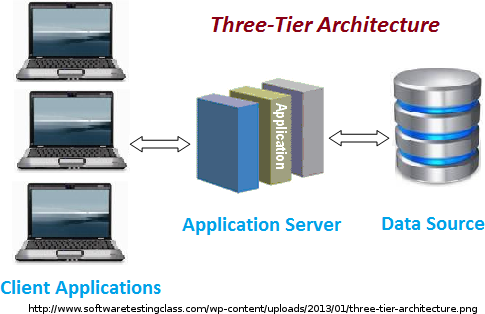
\includegraphics[height=0.25\pdfpageheight]{pic0008}
  \caption{Уеб базирана трислойна софтуерна архитектура.}
\label{fig:pic0008}
\end{figure}

При реализацията на настоящата система за изчисления в разпределена среда\index{изчисления в разпределена среда} изборът пада върху класическа трислойна софтуерна архитектура. Същият подход за три слоя се прилага и при реализацията на мобилното приложение, където SQLite локално съхранява данните над които се работи, Java обектно-ориентиран код извършва изчисленията, а Android базиран графичен потребителски интерфейс поема отговорността за визуализацията на процеса пред потребителя. 

\subsection{Подход за разработка}

\begin{figure}[h]
  \centering
  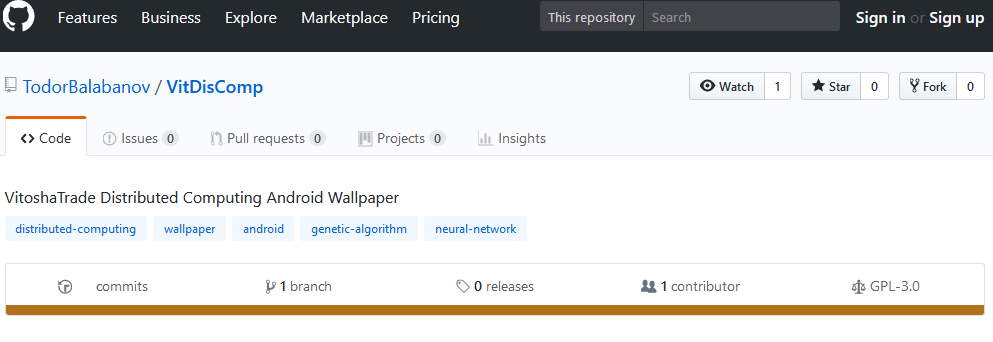
\includegraphics[width=1.0\linewidth]{pic0009}
  \caption{Подходи за софтуерна разработка.}
\label{fig:pic0009}
\end{figure}

Ако приемем, че визуализацията е най-горният слой, а базата данни най-долният слой на една трислойна софтуерна архитектура, то има два основни подхода за изработване на софтуерната система (Фиг. \ref{fig:pic0009}). При първия подход първоначално се разработва визуалния интерфейс, след това слоя на работната логика и накрая базата данни. Този подход се нарича „top-down“и е полезен когато се анализира софтуерно задание при което вече има в употреба множество хартиени документи (първоизточници на работните екрани. Този подход също е удобен при проекти с малък размер, където базата данни е относително опростена. Вторият много популярен подход е когато се започне с проектирането на базата данни, след това работната логика която обработва данните и едва накрая екраните визуализиращи информацията. Този подход се нарича „bottom-up“ и е най-подходящ когато се разработва сложно софтуерно решение, което се очаква да работи с големи обеми данни и множество различни структури на информацията. Акцентът в настоящата разработка е върху изчисленията които мобилните устройства извършват, а не толкова към създаването на голям масив от данни. Поради тази причина изборът в случая пада върху подхода „top-down“. 

\section{Лиценз и хранилище за проекта}

При съвременните софтуерни проекти с отворен код са от значение две неща – юридическият лиценз\index{софтуерни лицензи} под който съществува проекта и публичното хранилище\index{хранилища за програмен код} в което е разположен програмният текст. 

\subsection{Лиценз}

От съществено значение е изборът на правилен софтуерен лиценз, когато се разработва софтуерен проект предвиден да бъде публично достъпен. Съществуват множество възможности, като някои от най-популярните са - BSD License, MIT license, Mozilla Public License и GNU General Public License. За нуждите на настоящата разработка е предпочетен GNU General Public License v3, защото този лиценз е най-предпазващ за създателя на софтуерния продукт. В най-общи линии GPL3 позволява - комерсиална употреба, модификации, разпространение, включване в патенти и употреба за лични нужди. Лицензът съпровожда изключително ограничена отговорност за създателите на продукта и абсолютно никаква гаранция за употребата му от страна на потребителите. Лицензът също налага и серия ограничения – задължително включване на текст за авторските права на създателите, списък на извършените промени, не позволява закриване на кода и задължава всяко надграждане на продукта да бъде под същия лиценз. Със своята протекционистка природа GPL е един от лицензите дал най-силен тласък в развитието на продукти с отворен код, което е достатъчна причина да бъде избран за разработки без ясно изразена комерсиална насоченост. 

\subsection{Хранилище за програмен код}

Прието е всеки проект да има название, което особено важи в света на софтуера с отворен код. За настоящата разработка е избрано името VitDisComp. Точно това название е избрано, тъй като разработката ще се възползва от наличното сървър решение в проекта VIToshatrade \cite{vtrade} и по своята същност проектът е DIStributed COMPuting решение. 

\begin{figure}[h]
  \centering
  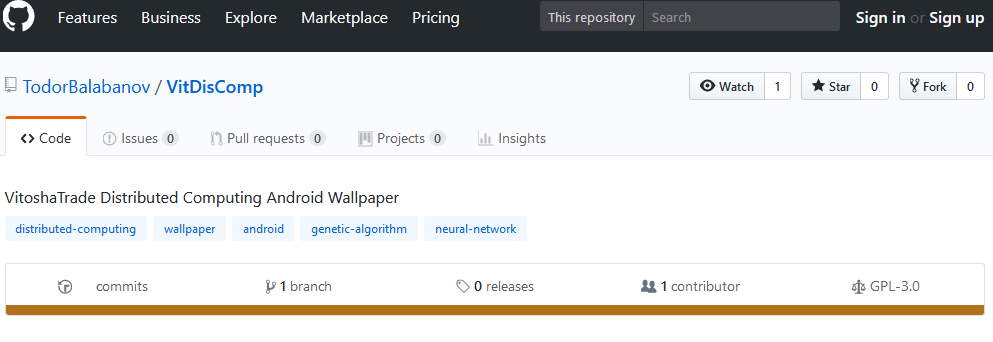
\includegraphics[width=1.0\linewidth]{pic0010}
  \caption{Публикуване на проект в GitHub.}
\label{fig:pic0010}
\end{figure}

Съществуват различни възможности за публикуване на програмния код, но една от най-популярните алтернативи е облачната услуга GitHub. Услугата GitHub (Фиг. \ref{fig:pic0010}) е базирана на системата за контрол на версиите Git и дава една от най-широките възможности за популяризиране на програмен код с отворен лиценз.
\newpage
\chapter{Android Live Wallpaper}
\label{chapter04}

Android Live Wallpaper technology provides animated visual representation capabilities in virtual wallpaper. This type of application does not differ drastically from other Android applications and can perform almost all of their capabilities. Since the virtual wallpaper is always active, it is an ideal candidate for implementing background computing\index{distributed computing}. The following components are required to create an active wallpaper: 1. An XML file that describes the components of the wallpaper; 2. Background module (Android Service); 3. Appropriate permissions to access device resources.

\section{Mobile App Manifest File}

When creating applications for the Android operating system, the approach adopted is to describe the components of the mobile application in a manifest file (AndroidManifest.xml) using XML syntax.

\begin{figure}[h]
\centering
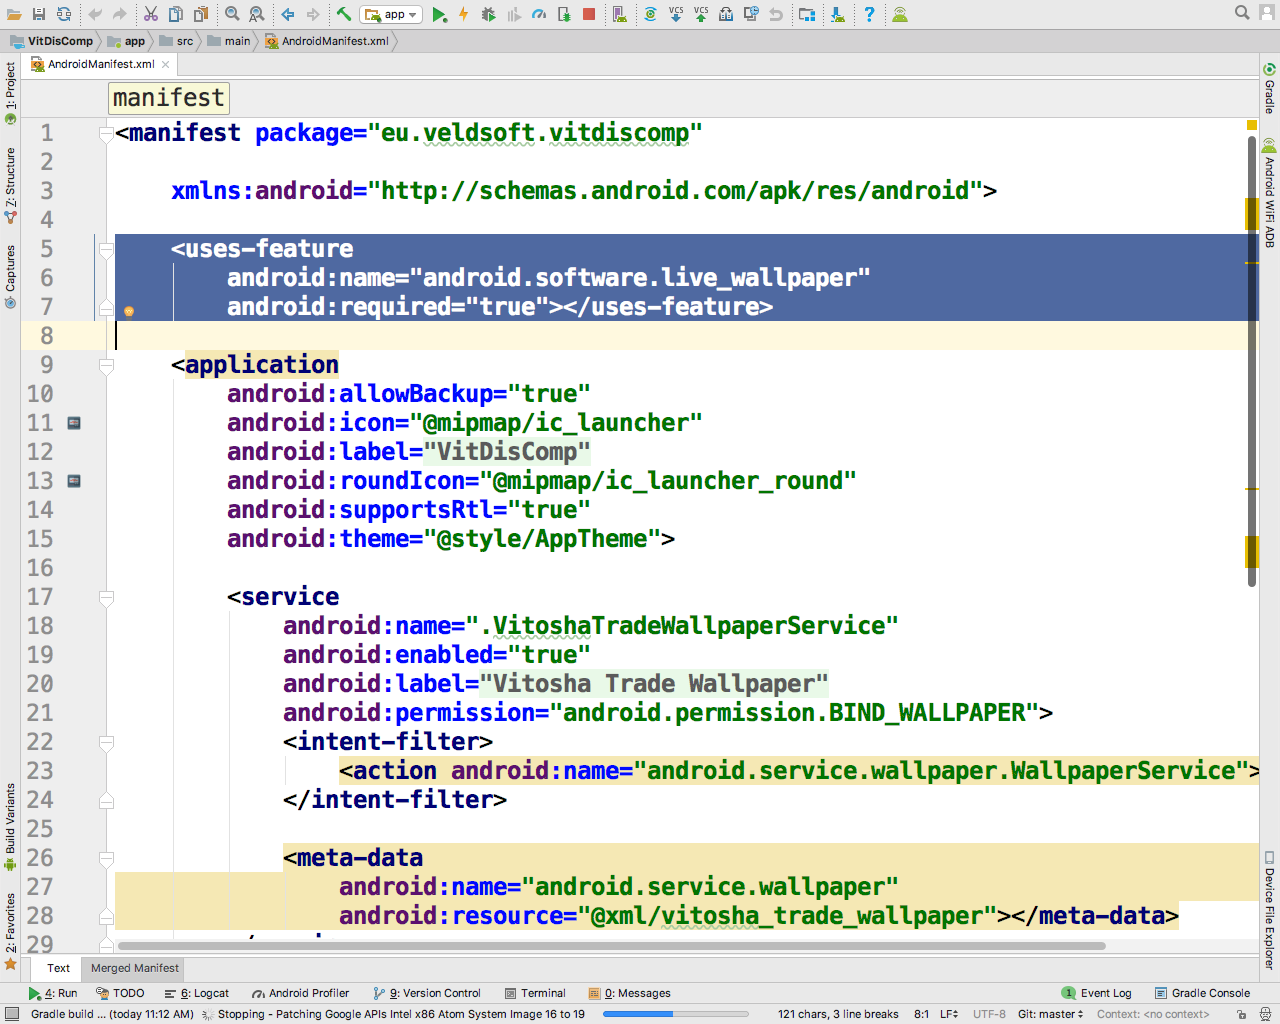
\includegraphics[height=0.45\pdfpageheight]{pic0011}
\caption{Setting the app as active wallpaper}
\label{fig:pic0011}
\end{figure}
\FloatBarrier

To define the application as an active wallpaper application, mark it explicitly in the manifest file (Fig. \ref{fig:pic0011}). The most significant benefit of this definition is that it prevents the application from being installed on devices that do not support live wallpaper rendering capabilities.

\begin{figure}[h]
\centering
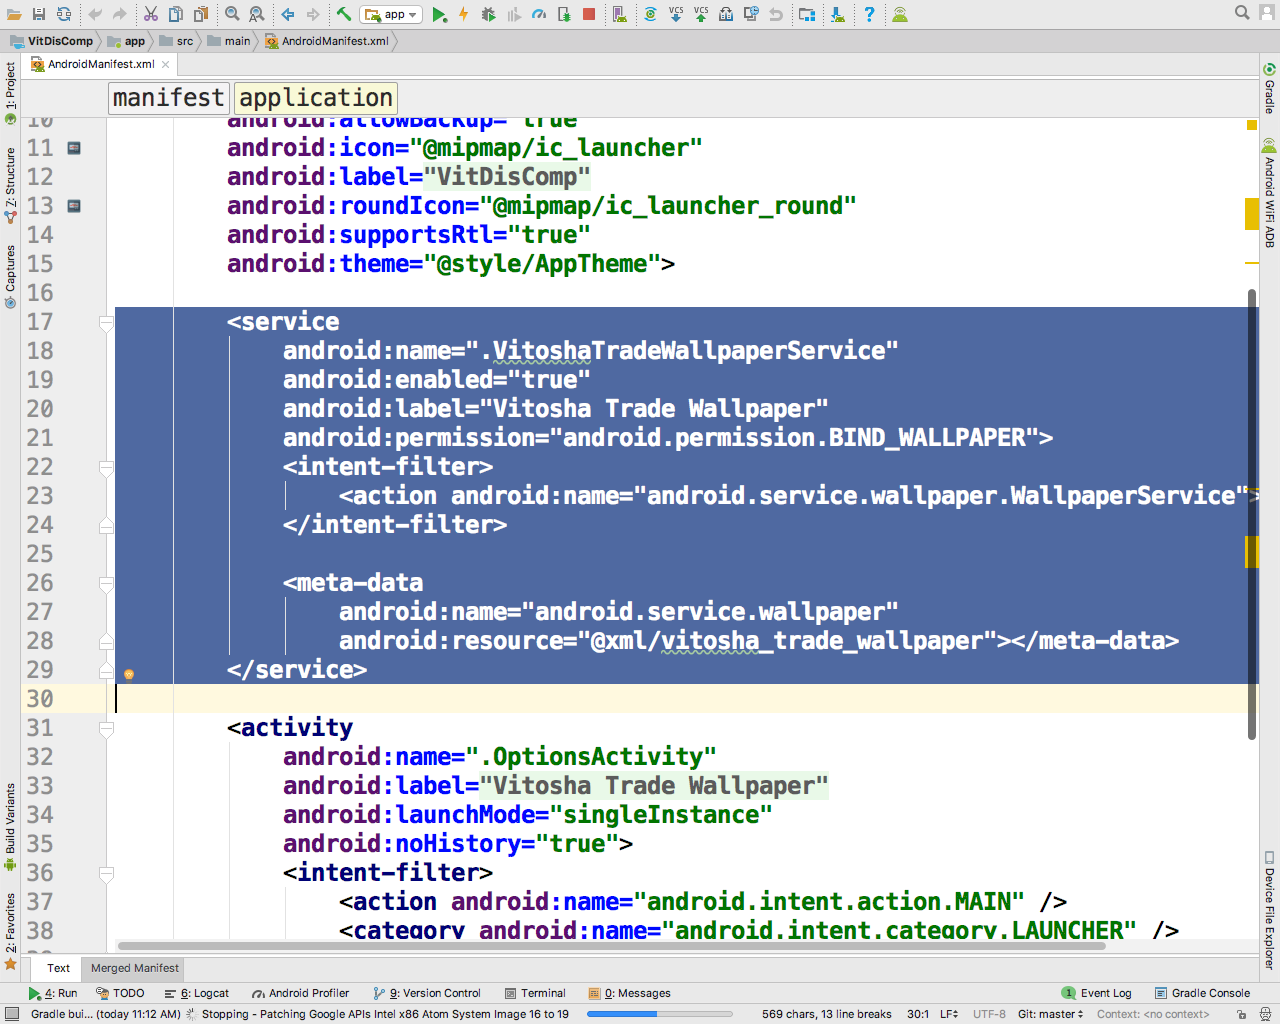
\includegraphics[height=0.45\pdfpageheight]{pic0012}
\caption{Module of type ``service''}
\label{fig:pic0012}
\end{figure}
\FloatBarrier

When an Android application uses very long calculations that are not convenient to perform on the main GUI thread, it is common for a thread to export them to non-GUI modules called "services". The work of the active wallpaper is carried out in just such a module, and for this reason, one has been added to the project (Fig. \ref{fig:pic0012}).

\begin{figure}[h]
\centering
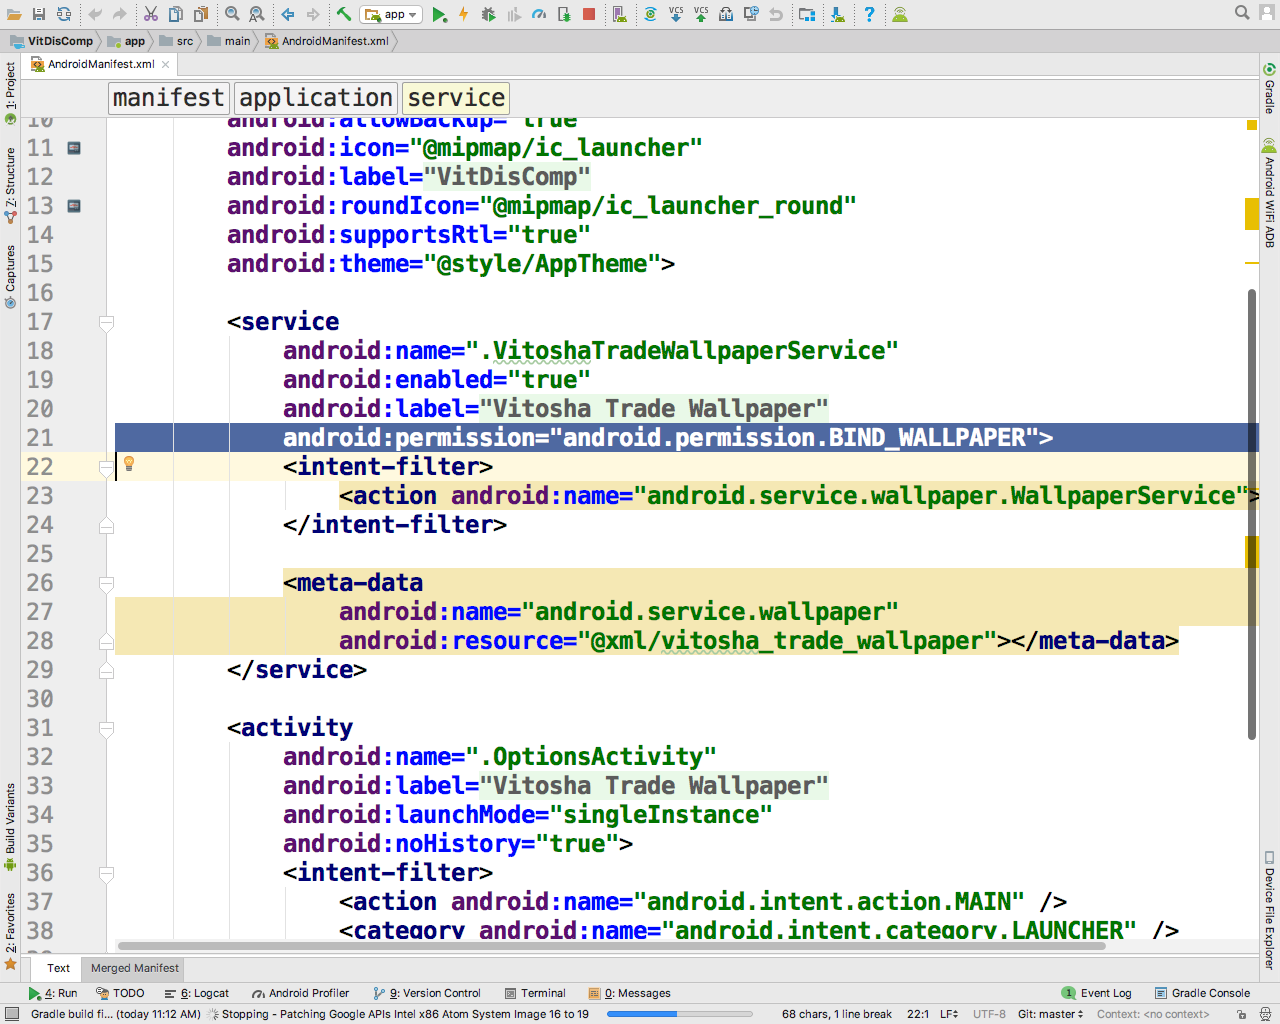
\includegraphics[height=0.45\pdfpageheight]{pic0013}
\caption{Active wallpaper resource access flags}
\label{fig:pic0013}
\end{figure}
\FloatBarrier

The security model requires the user's explicit consent to be obtained for any more specific action, in the case of the active wallpaper, the addition of the android.permission.BIND\_WALLPAPER permission is required (Fig. \ref{fig:pic0013}).

\begin{figure}[h]
\centering
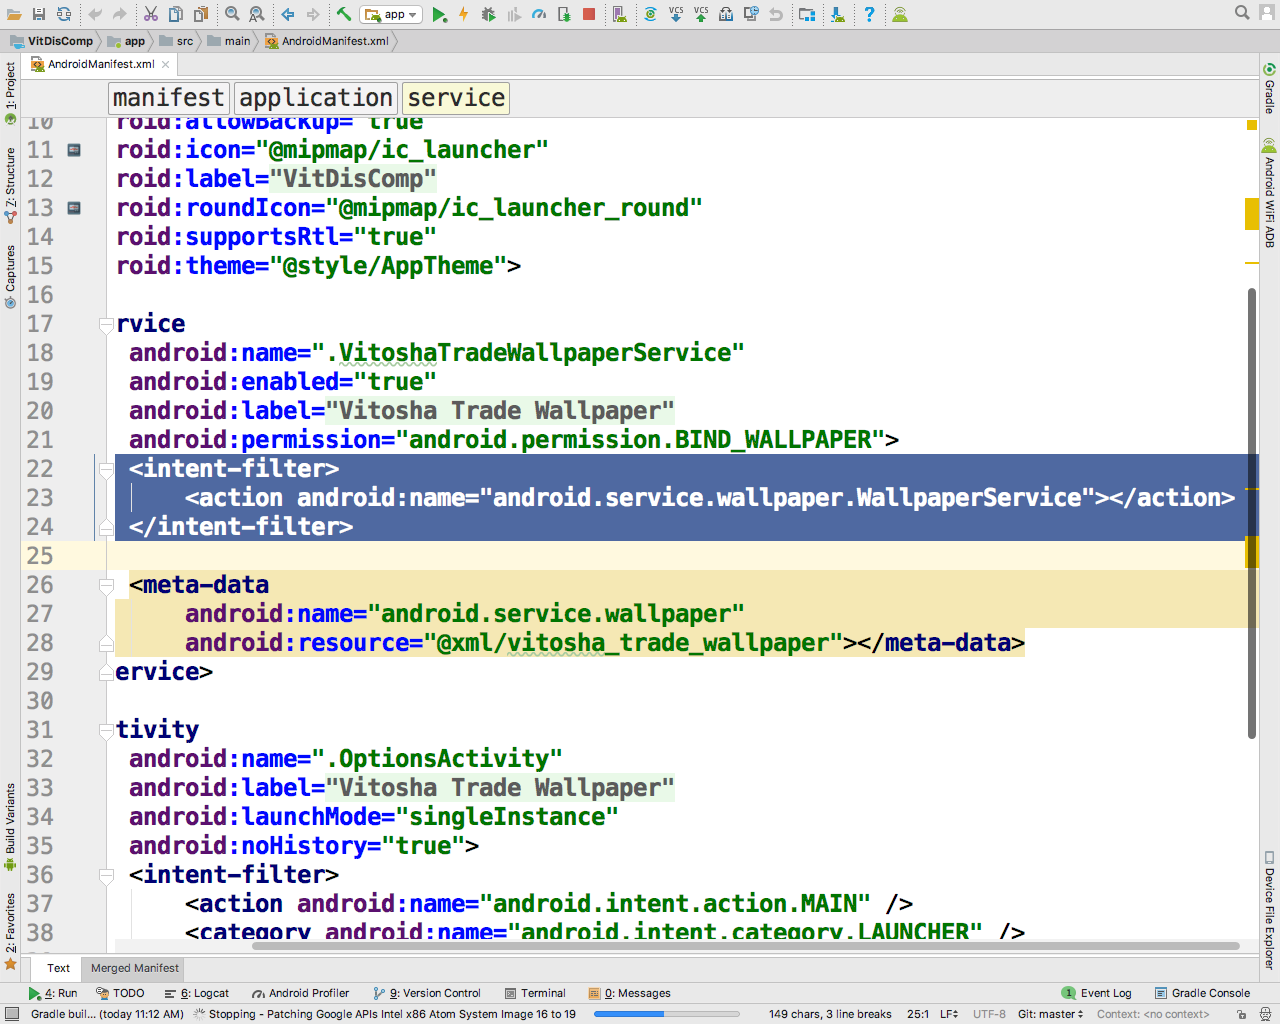
\includegraphics[height=0.45\pdfpageheight]{pic0014}
\caption{Operating system message listening service registration.}
\label{fig:pic0014}
\end{figure}
\FloatBarrier

In addition to the need for permission to use the active wallpaper resources, the service needs to be subscribed to listen for messages from the operating system (Fig \ref{fig:pic0014}).

\begin{figure}[h]
\centering
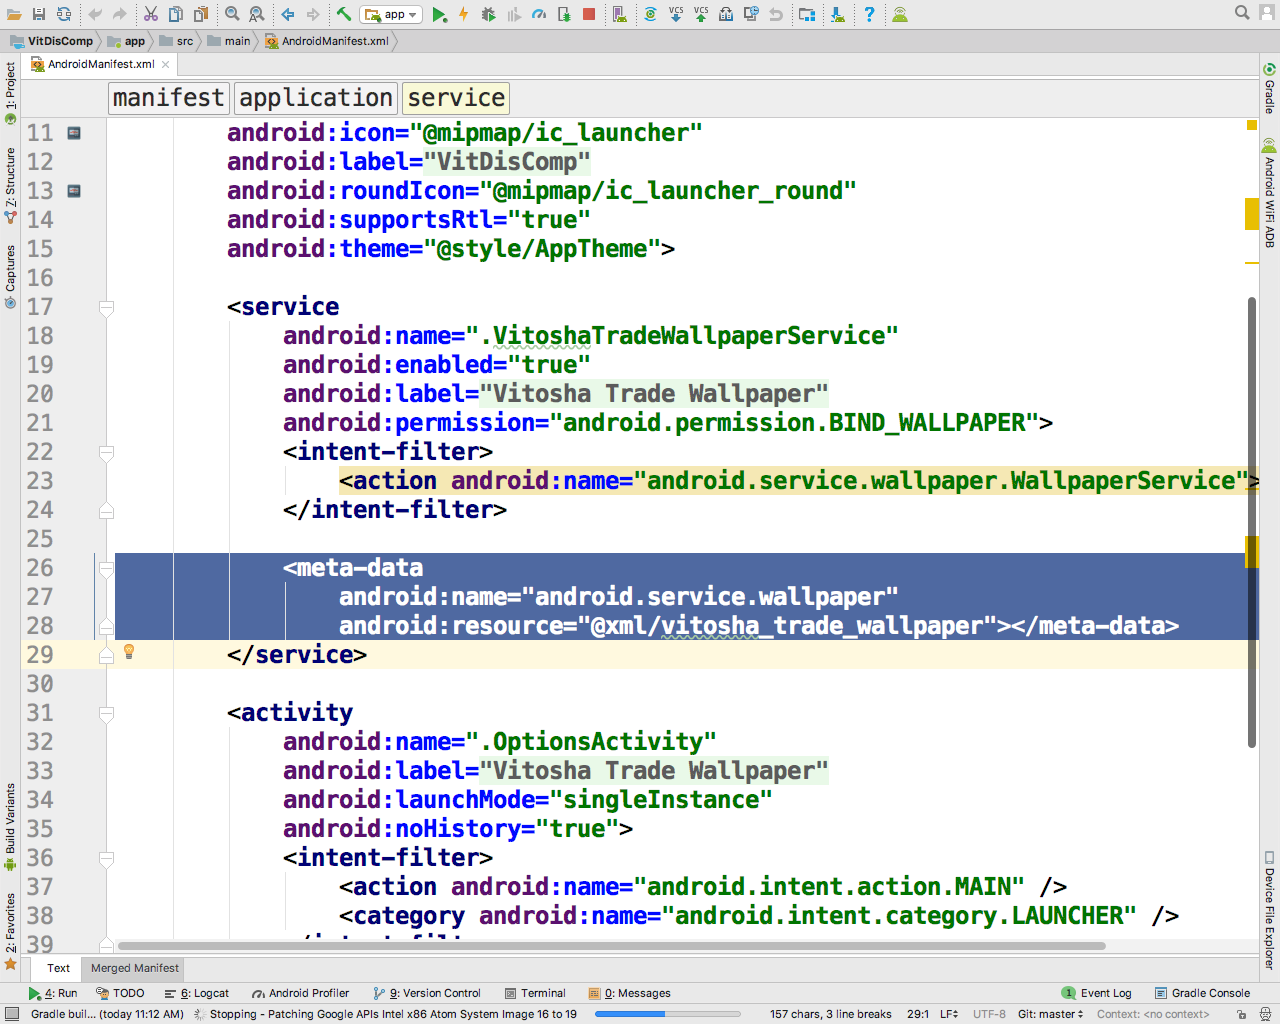
\includegraphics[height=0.45\pdfpageheight]{pic0015}
\caption{Reference to active wallpaper description file}
\label{fig:pic0015}
\end{figure}
\FloatBarrier

The description of the active wallpaper itself is contained in a separate XML file, a reference indicated in the manifest (Fig. \ref{fig:pic0015}).

\begin{figure}[h]
\centering
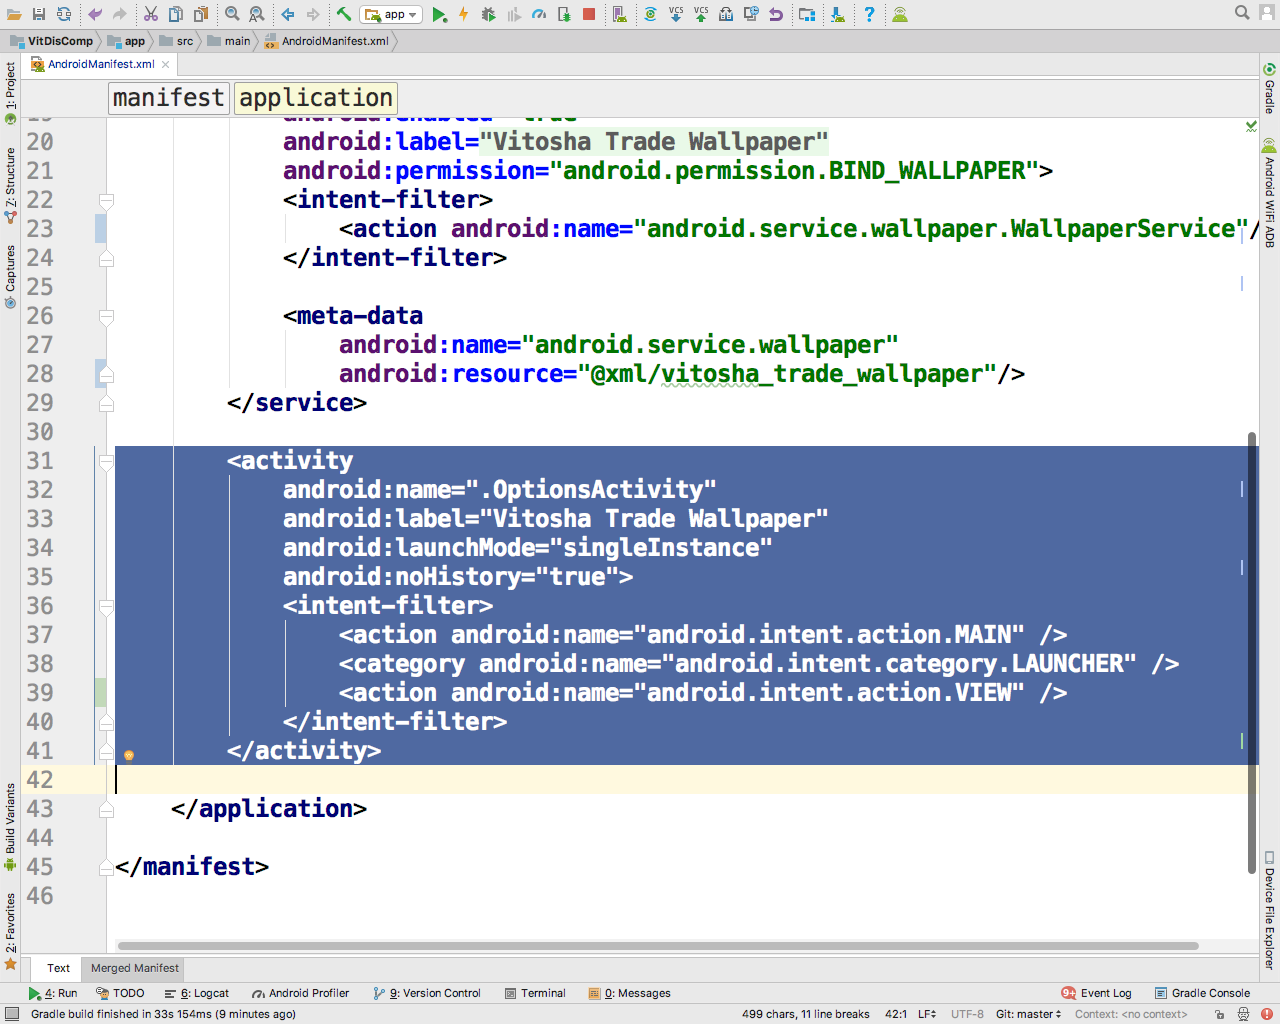
\includegraphics[height=0.45\pdfpageheight]{pic0016}
\caption{Window to set active wallpaper}
\label{fig:pic0016}
\end{figure}
\FloatBarrier

The last component in such an application is a window (Android Activity) to be launched by the operating system and serve to establish the active wallpaper (Fig. \ref{fig:pic0016}). In this case, the possibility is used that this launch window also combines the functions of a window with options (Preference Activity).

\begin{figure}[h]
\centering
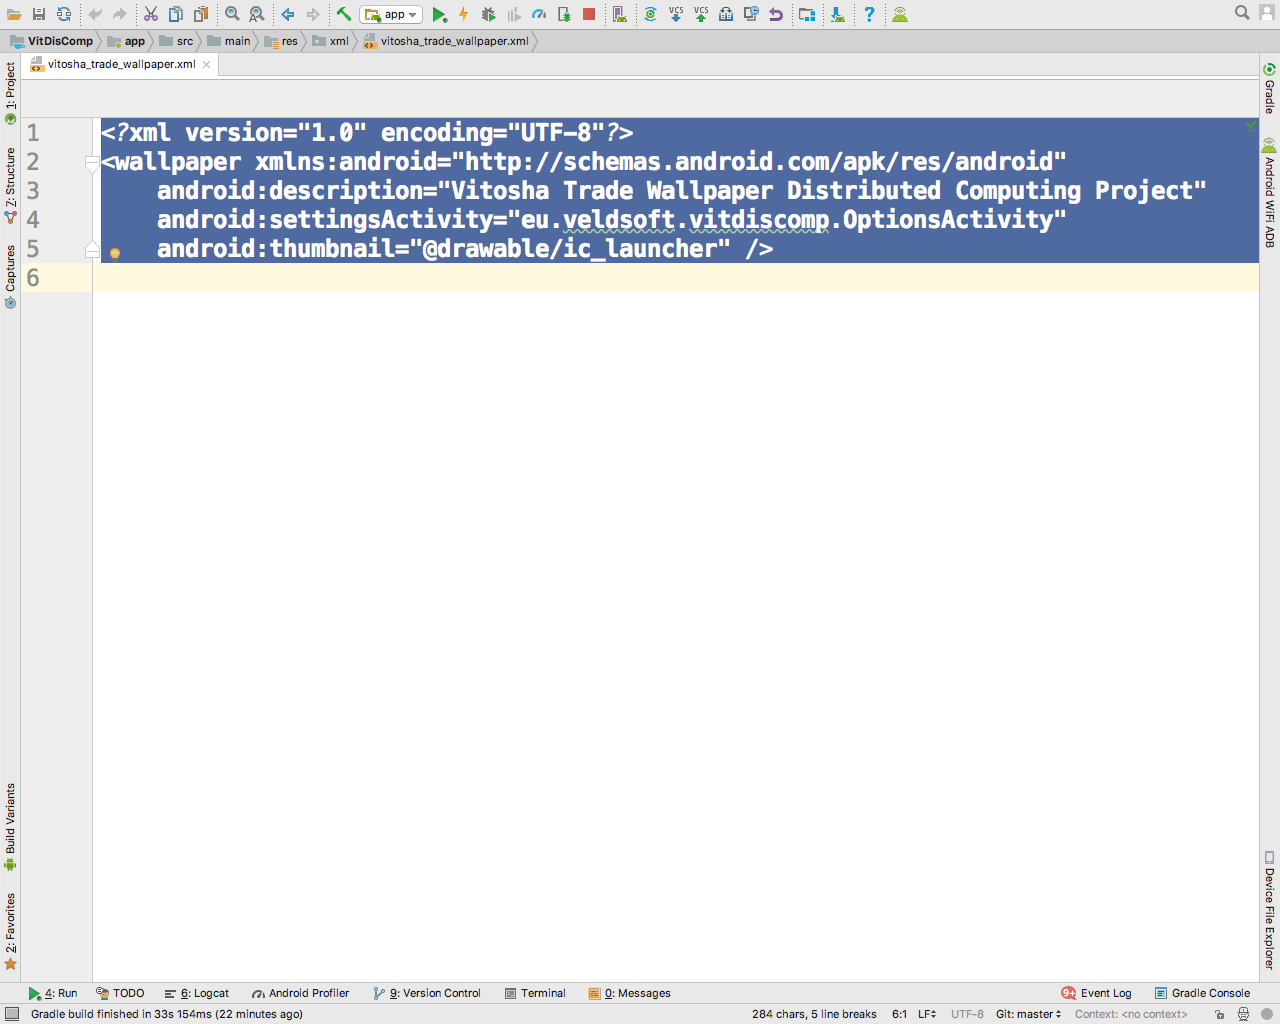
\includegraphics[height=0.45\pdfpageheight]{pic0017}
\caption{XML wallpaper description file}
\label{fig:pic0017}
\end{figure}
\FloatBarrier

As already mentioned, the active wallpaper is described in a separate XML file, which contains a short annotation of the application, a preview, a thumbnail icon, and the name of the settings window (Fig. \ref{fig:pic0017}).

\section{Settings Screen}

Since the active wallpaper will also have a secondary task of visualizing the progress of calculations, it is reasonable to create a settings window for it.

\begin{figure}[h]
\centering
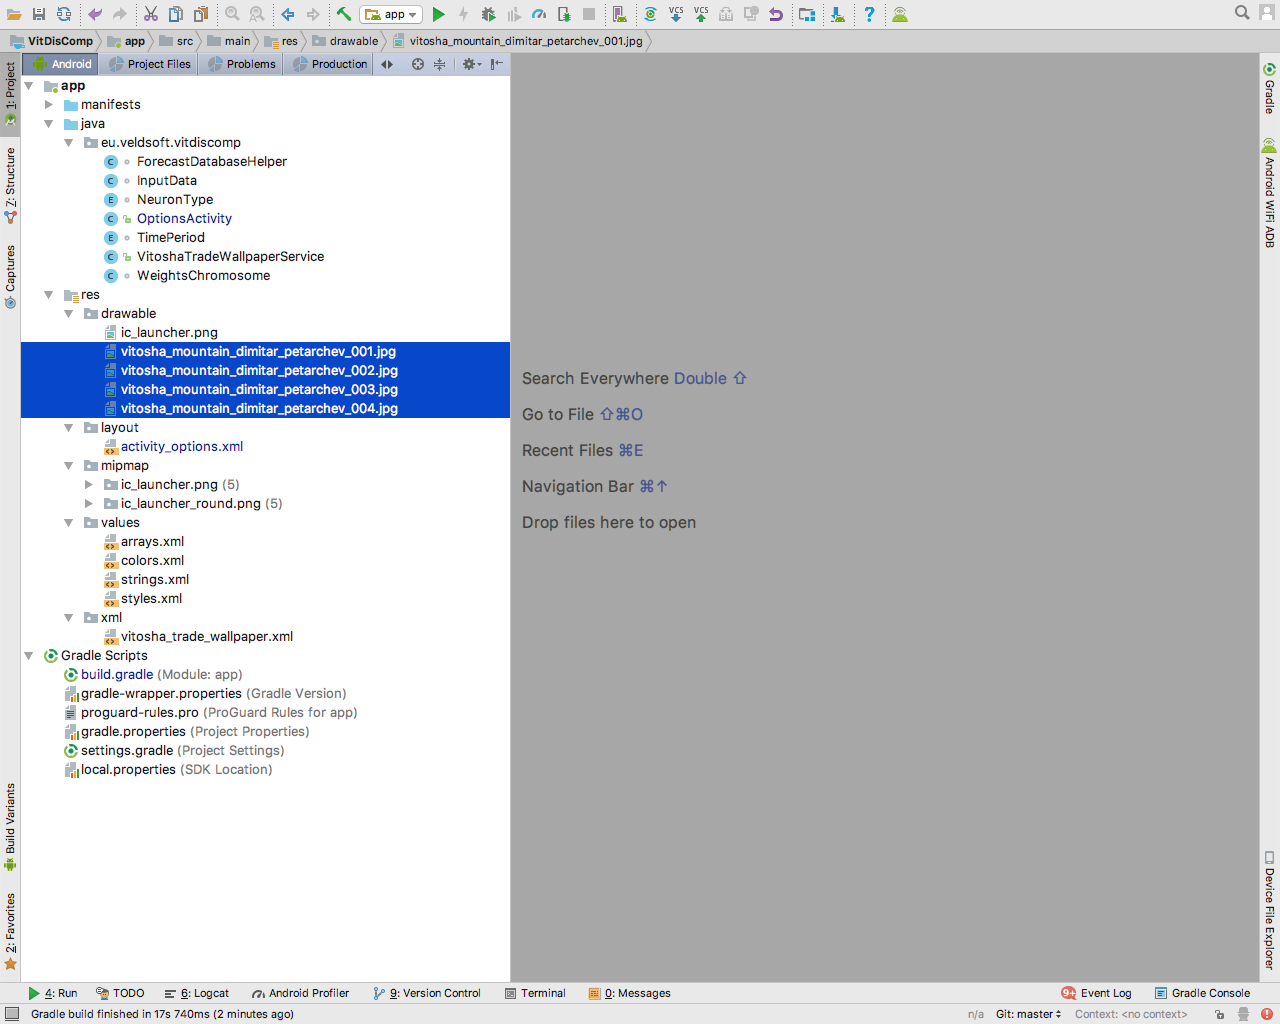
\includegraphics[height=0.45\pdfpageheight]{pic0018}
\caption{Graphic files containing photographs of Vitosha Mountain near the city of Sofia, Bulgaria}
\label{fig:pic0018}
\end{figure}
\FloatBarrier

As a visual representation, the simplest possible option has been chosen. Several photographs of the Vitosha mountain are visualized in the form of segments with the dimensions of the screen of the mobile device (Fig. \ref{fig:pic0018}). Three translucent areas visualize information about the financial time series (code and period), a bar chart about the input and output data, and the current state of the artificial neural network\index{artificial neural networks} (Fig. \ref{fig:pic0019} ).

\begin{figure}[h]
\centering
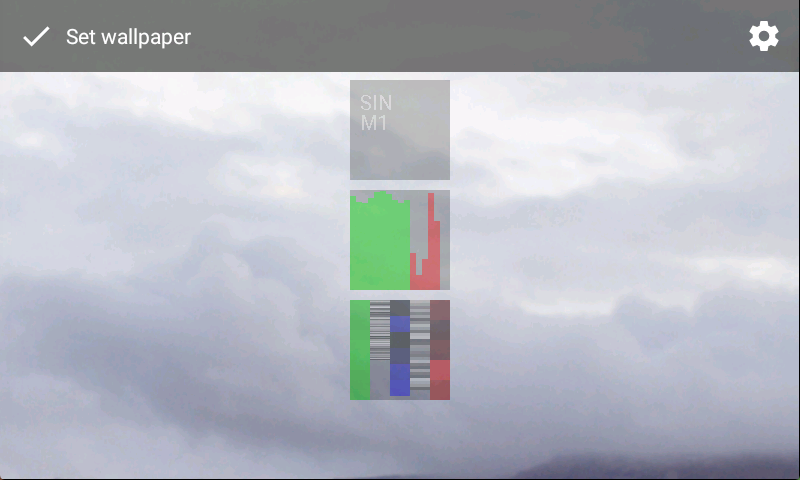
\includegraphics[width=1.0\linewidth]{pic0019}
\caption{Visual representation of information from calculations}
\label{fig:pic0019}
\end{figure}
\FloatBarrier

The live wallpaper settings provide position and size controls for the three visual areas. They also added initial settings for device load level and whether to enable active wallpaper (Fig \ref{fig:pic0020}).

\begin{figure}[h]
\centering
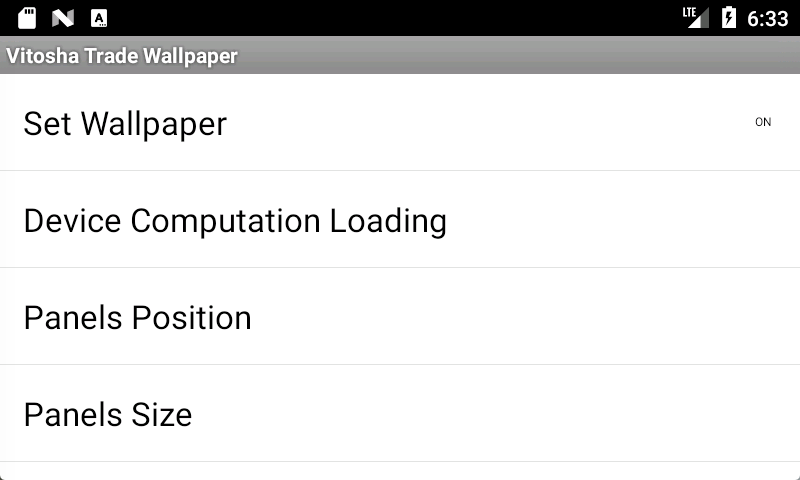
\includegraphics[width=1.0\linewidth]{pic0020}
\caption{Initial set of settings}
\label{fig:pic0020}
\end{figure}
\FloatBarrier

Each window in Android is described with its layout file and Java code file. A GUI descriptor file uses XML and is very similar to composing a web page. When designing a settings screen, one of the most valuable tools in the Android operating system is Shared Preferences. They allow the state of visual components to be directly stored in the device in the form of key-value pairs and then programmatically used for this information.

\subsection{Description of the user interface in the form of XML files}

\begin{figure}[h]
\centering
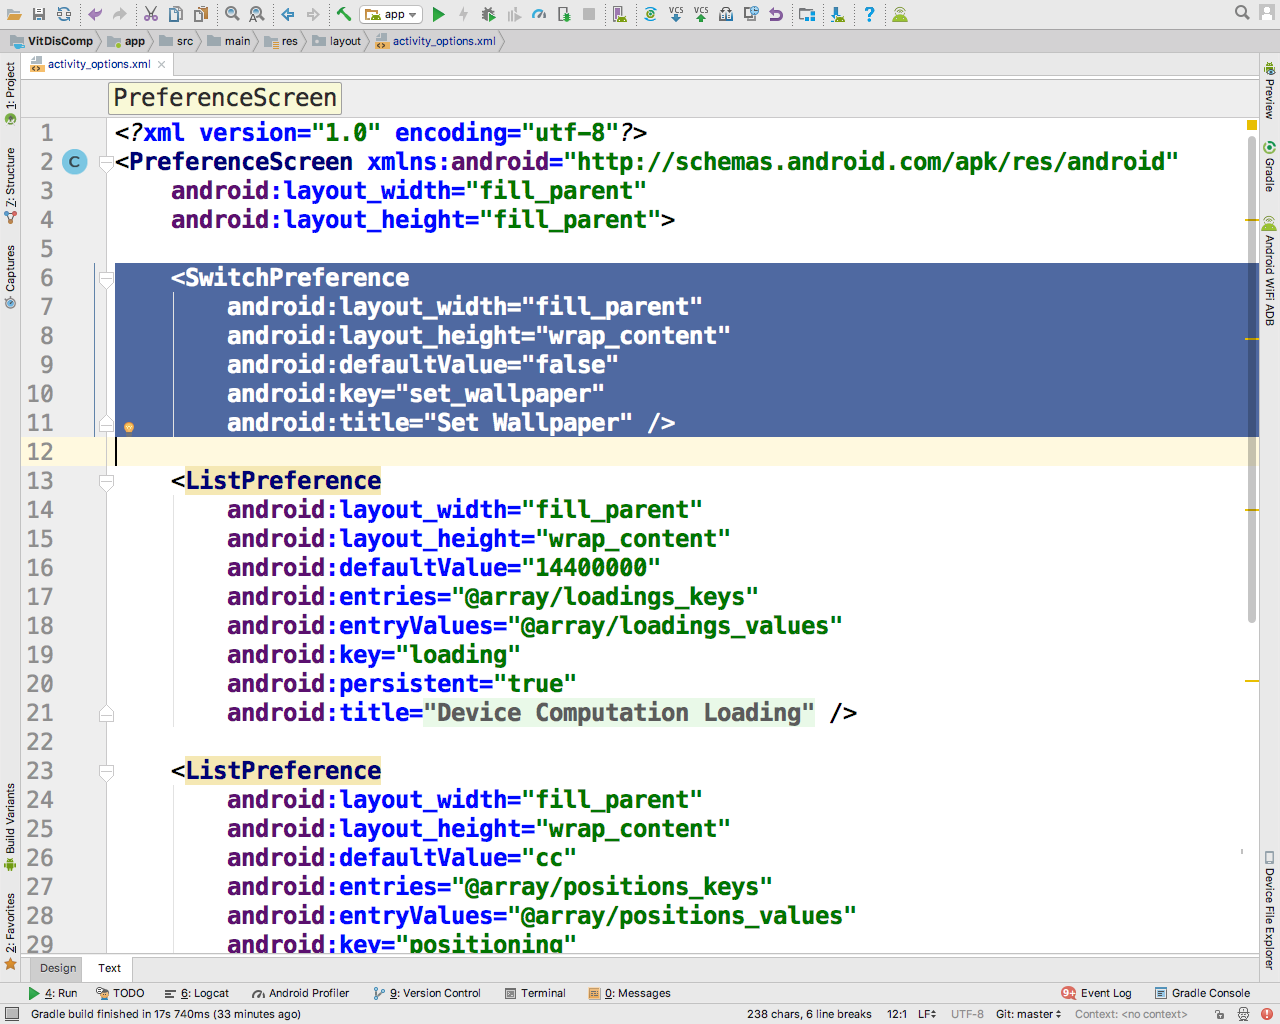
\includegraphics[height=0.45\pdfpageheight]{pic0021}
\caption{Visual component to turn wallpaper on and off}
\label{fig:pic0021}
\end{figure}
\FloatBarrier

First, there is a visual component for turning on and off the active wallpaper. When the switch is in the ON state, the active wallpaper is started, and when it is in the OFF position, the active wallpaper is disabled (Fig. \ref{fig:pic0021}).

\begin{figure}[h]
\centering
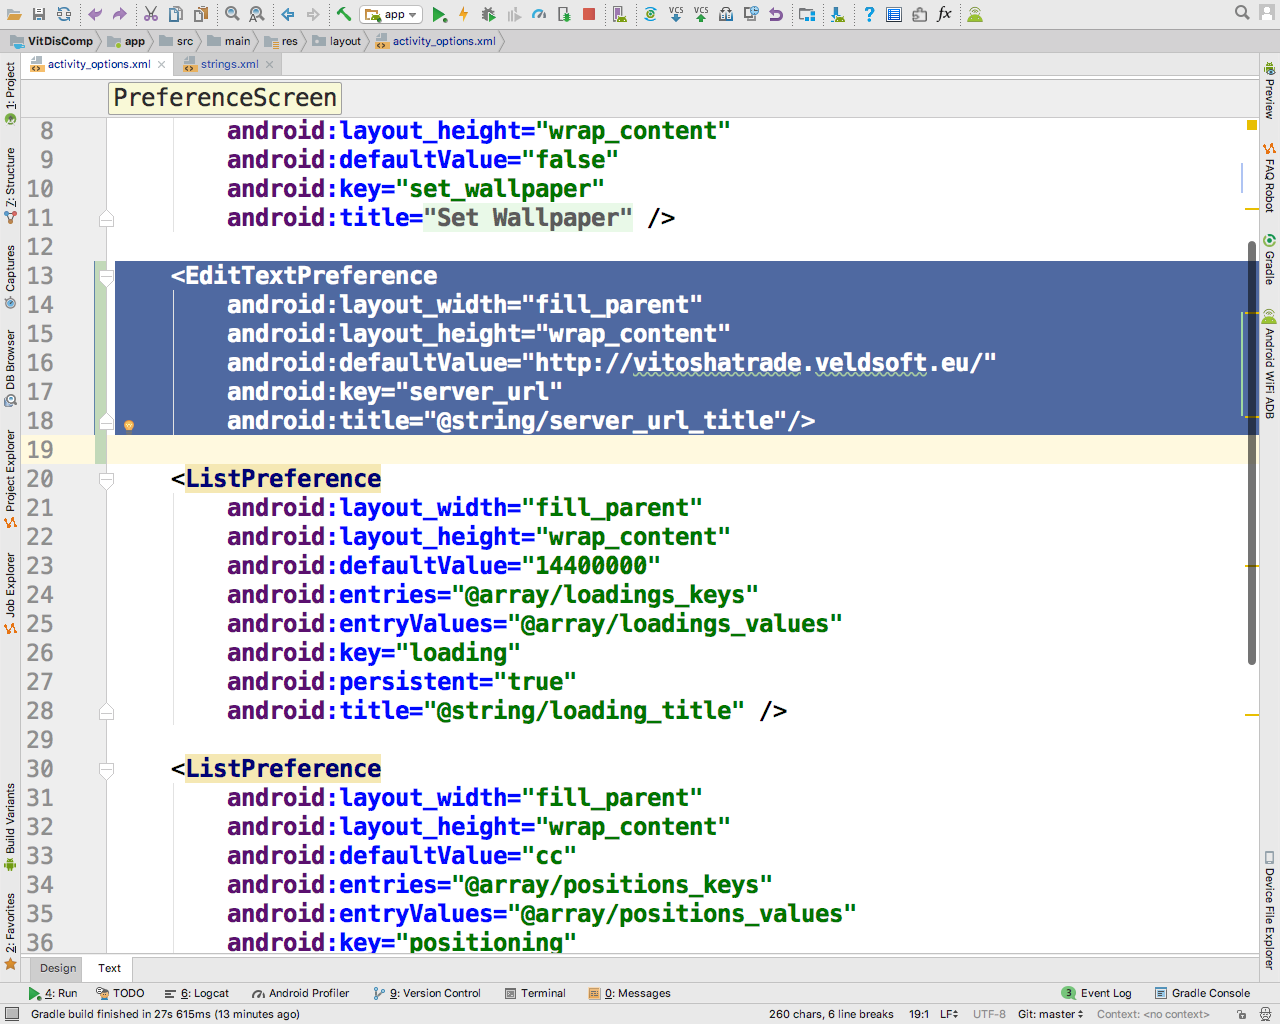
\includegraphics[height=0.45\pdfpageheight]{pic0154}
\caption{Visual Component for Specifying a Server URL}
\label{fig:pic0154}
\end{figure}
\FloatBarrier

Since the mobile application pulls the time series information from a remote web server, it is appropriate for the user to be able to set the URL of the server being worked with (Fig. \ref{fig:pic0154}). This option allows traffic to be redirected to other servers after the application is installed on users' mobile devices.

\begin{figure}[h]
\centering
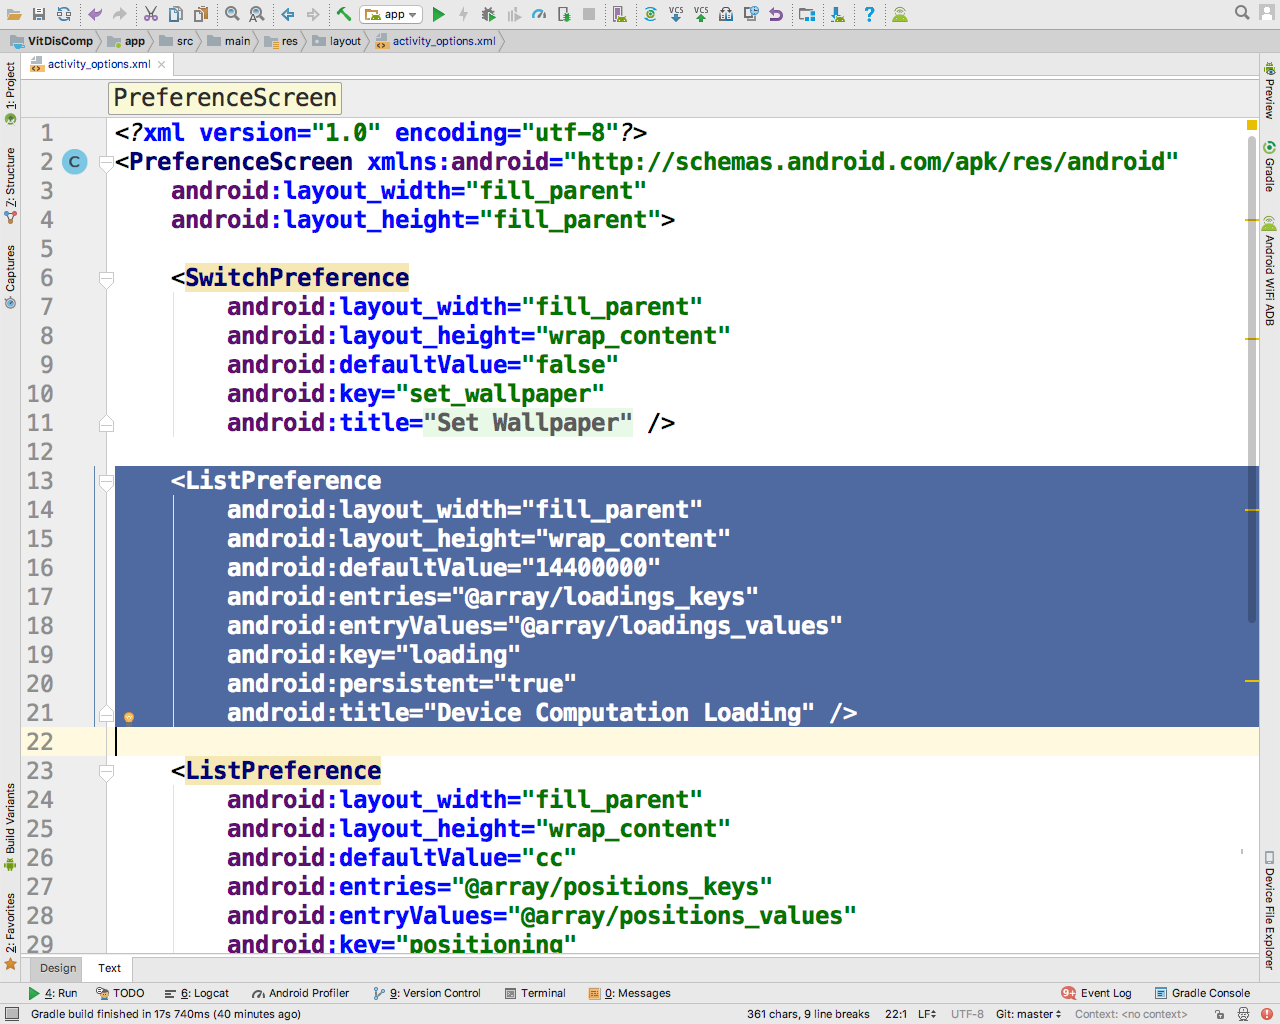
\includegraphics[height=0.45\pdfpageheight]{pic0022}
\caption{Visual load adjustment component}
\label{fig:pic0022}
\end{figure}
\FloatBarrier

A list of predefined values is used to load the device when performing the background calculations (Fig. \ref{fig:pic0022}).

\begin{figure}[h]
\centering
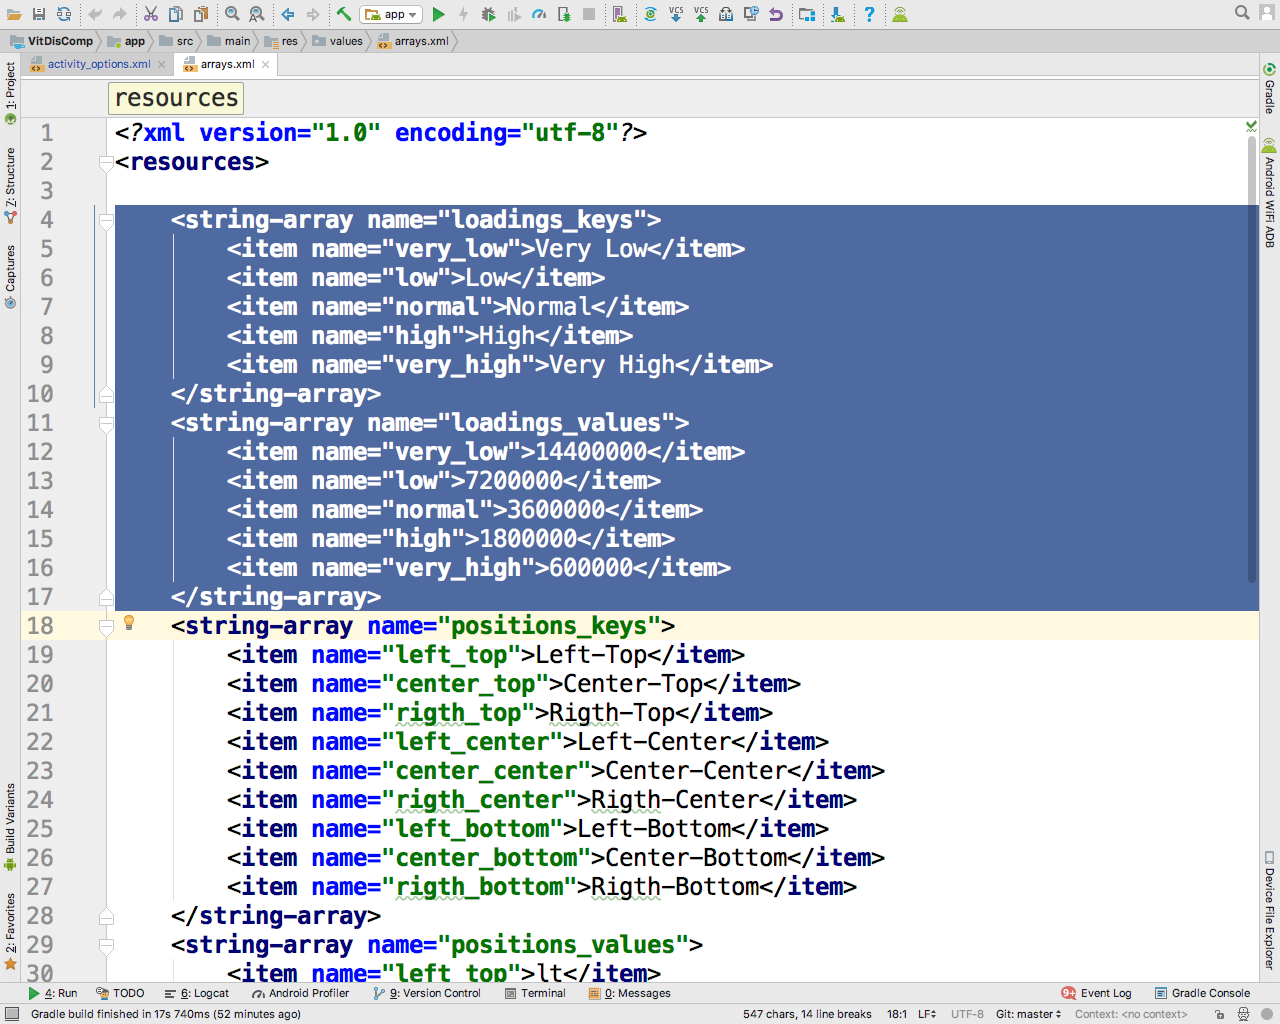
\includegraphics[height=0.45\pdfpageheight]{pic0023}
\caption{System Load Values}
\label{fig:pic0023}
\end{figure}
\FloatBarrier

When designing the Android system, one of the main goals was to separate the graphical interface from the data as much as possible. This is precisely why the load level values are exported in a separate resource (Fig. \ref{fig:pic0023}).

\begin{figure}[h]
\centering
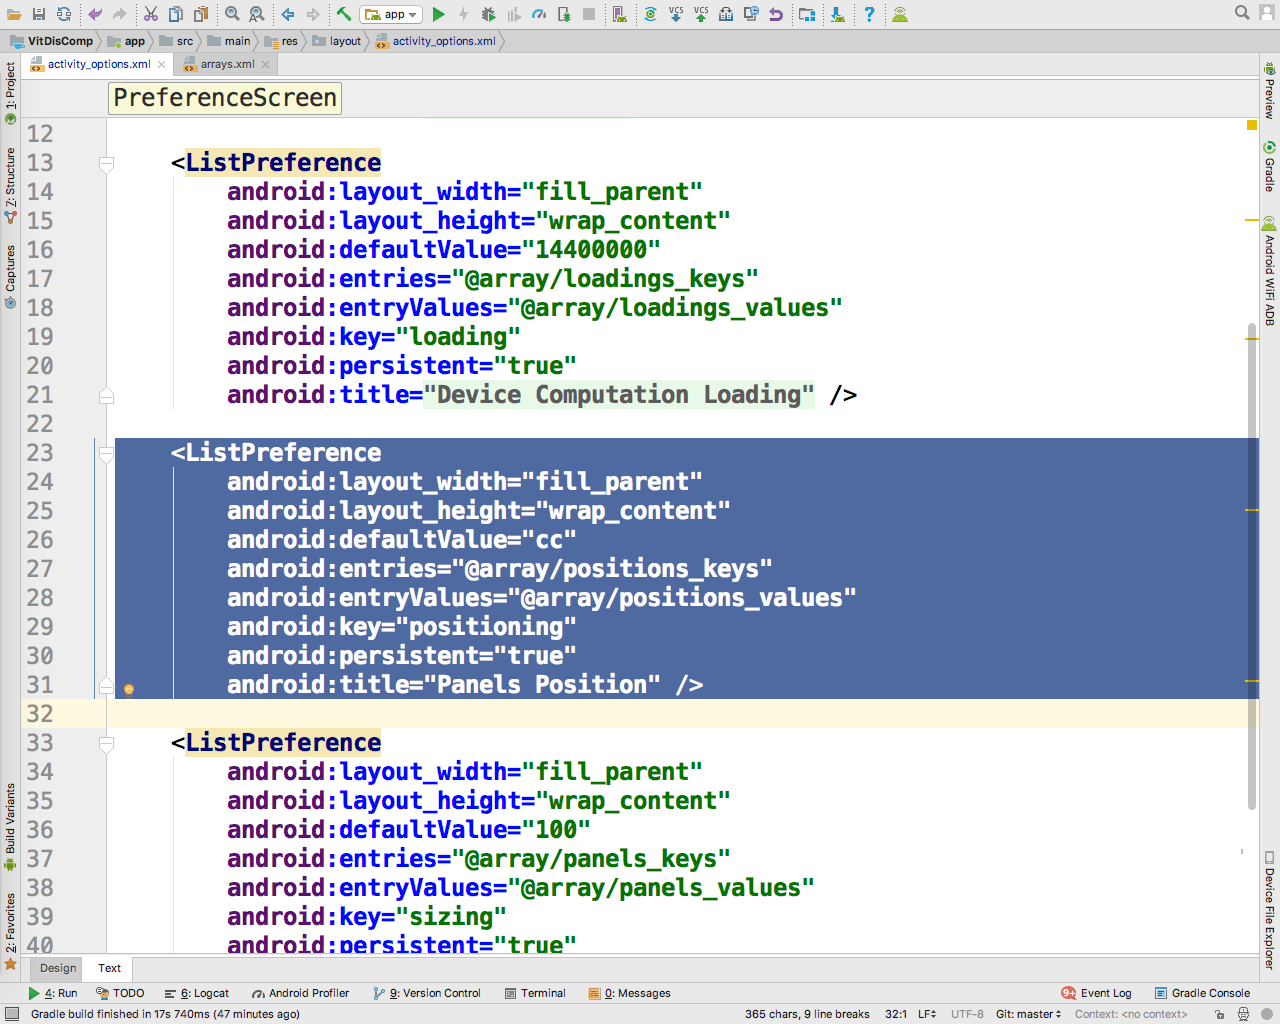
\includegraphics[height=0.45\pdfpageheight]{pic0024}
\caption{Positioning of visual presentation areas}
\label{fig:pic0024}
\end{figure}
\FloatBarrier

The positioning of the visual representation areas is also adjusted by selecting values from a list (Fig. \ref{fig:pic0024}).

\begin{figure}[h]
\centering
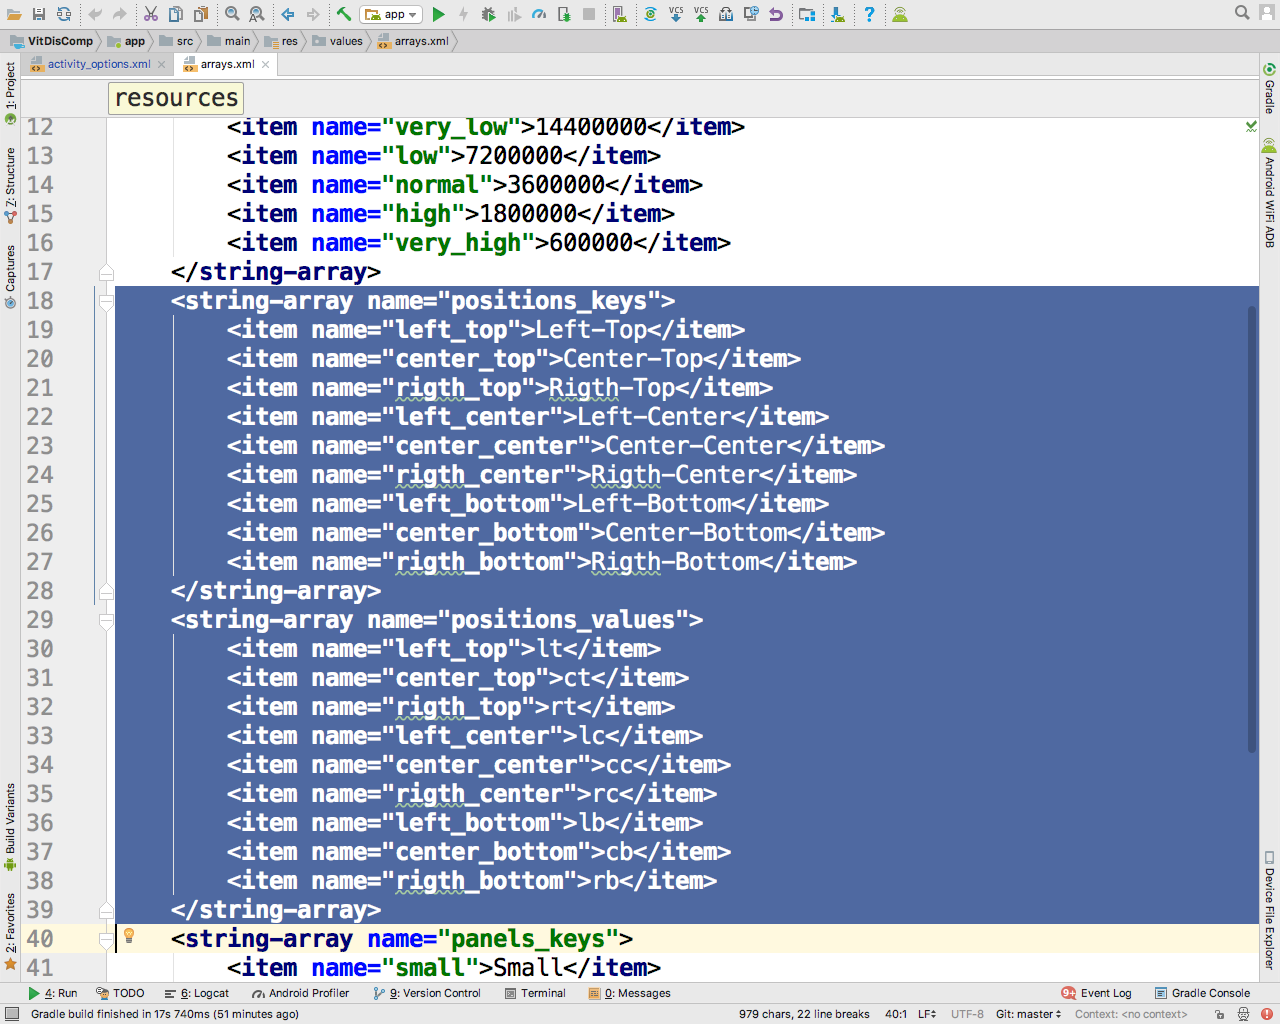
\includegraphics[height=0.45\pdfpageheight]{pic0025}
\caption{Position values for visual representation areas}
\label{fig:pic0025}
\end{figure}
\FloatBarrier

Analogously to the load level values, the list of possible positions of the visual representation areas is exported in a separate resource file (Fig. \ref{fig:pic0025}).

\begin{figure}[h]
\centering
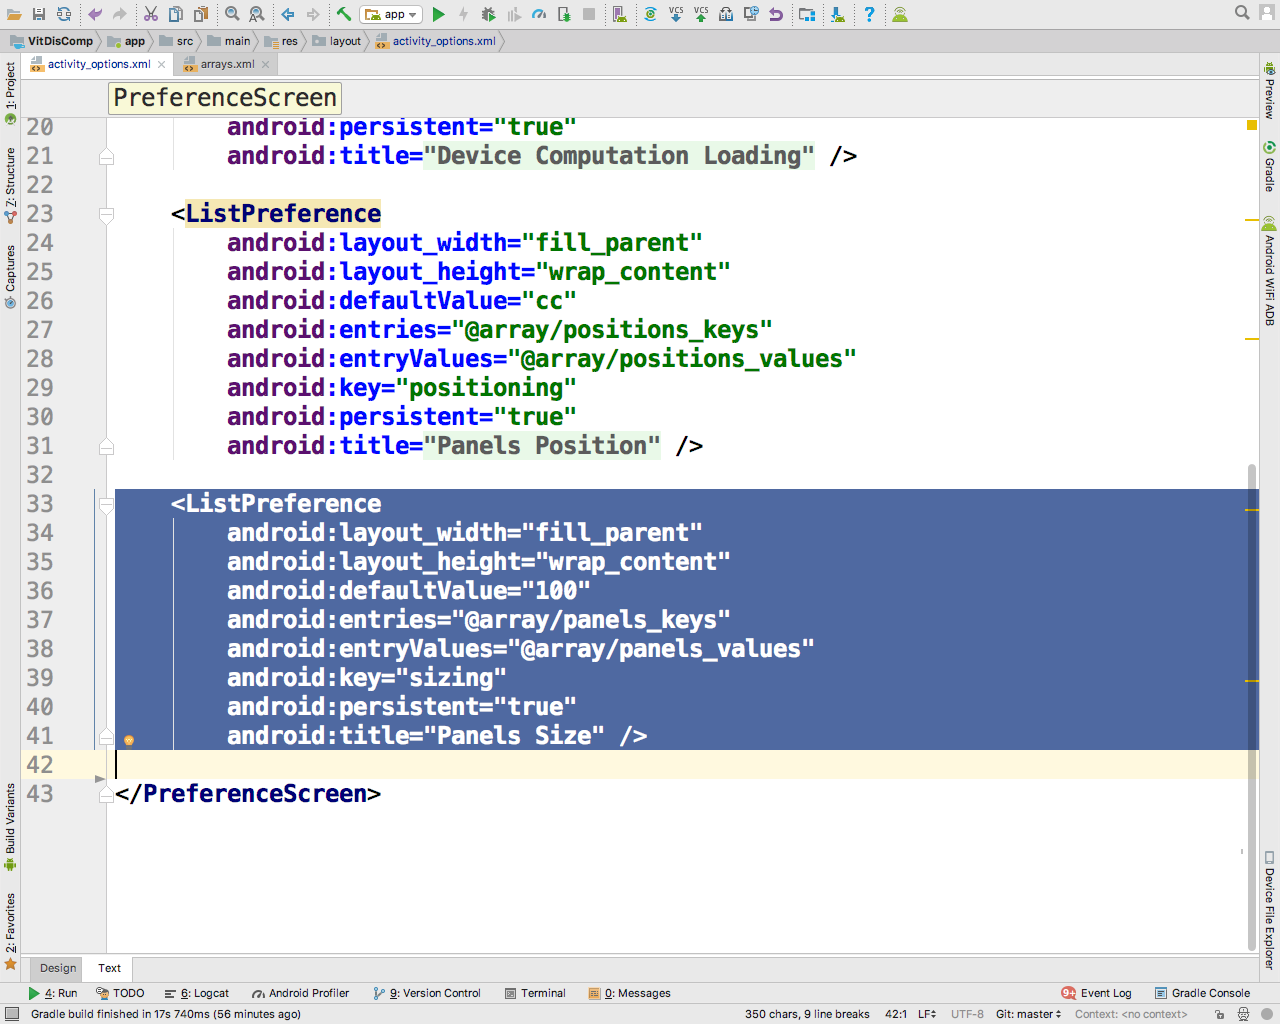
\includegraphics[height=0.45\pdfpageheight]{pic0026}
\caption{Size of visual representation areas}
\label{fig:pic0026}
\end{figure}
\FloatBarrier

Of the initial characteristics, the last is the size of the areas for the visual presentation of information (Fig. \ref{fig:pic0026}).

\begin{figure}[h]
\centering
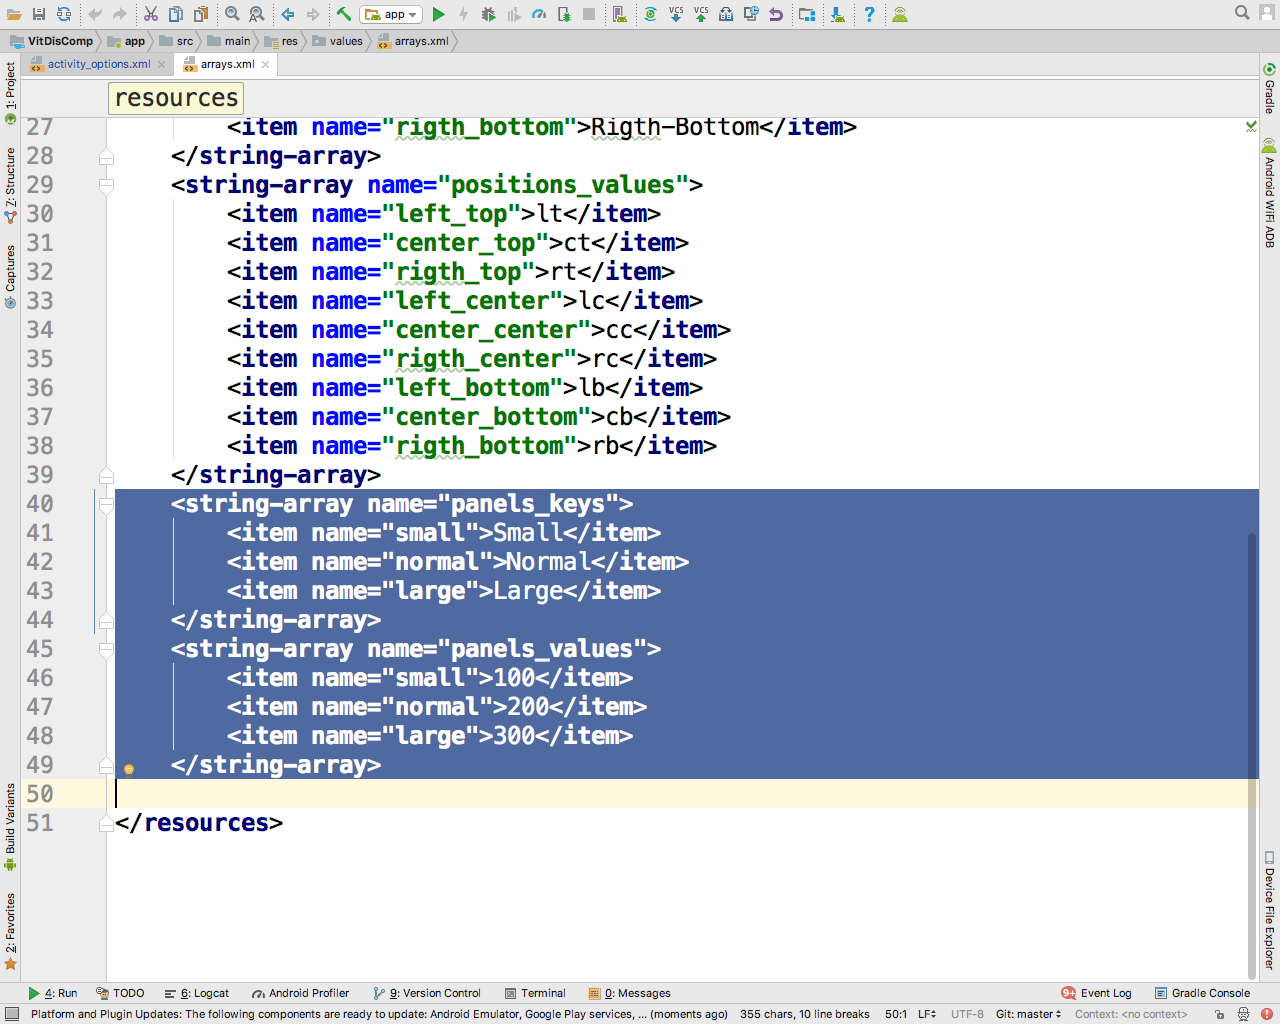
\includegraphics[height=0.45\pdfpageheight]{pic0027}
\caption{Size values for visual representation areas}
\label{fig:pic0027}
\end{figure}
\FloatBarrier

Areas for the visual representation of information are available in three sizes small, medium, and large (Fig. \ref{fig:pic0027}).

\subsection{Interface Control Program Code}

Events raised by the GUI are intercepted in specially written Java functions so that when they are activated, the necessary programmatic actions are performed. Only two events are caught for the settings screen - create and pause.

\begin{figure}[h]
\centering
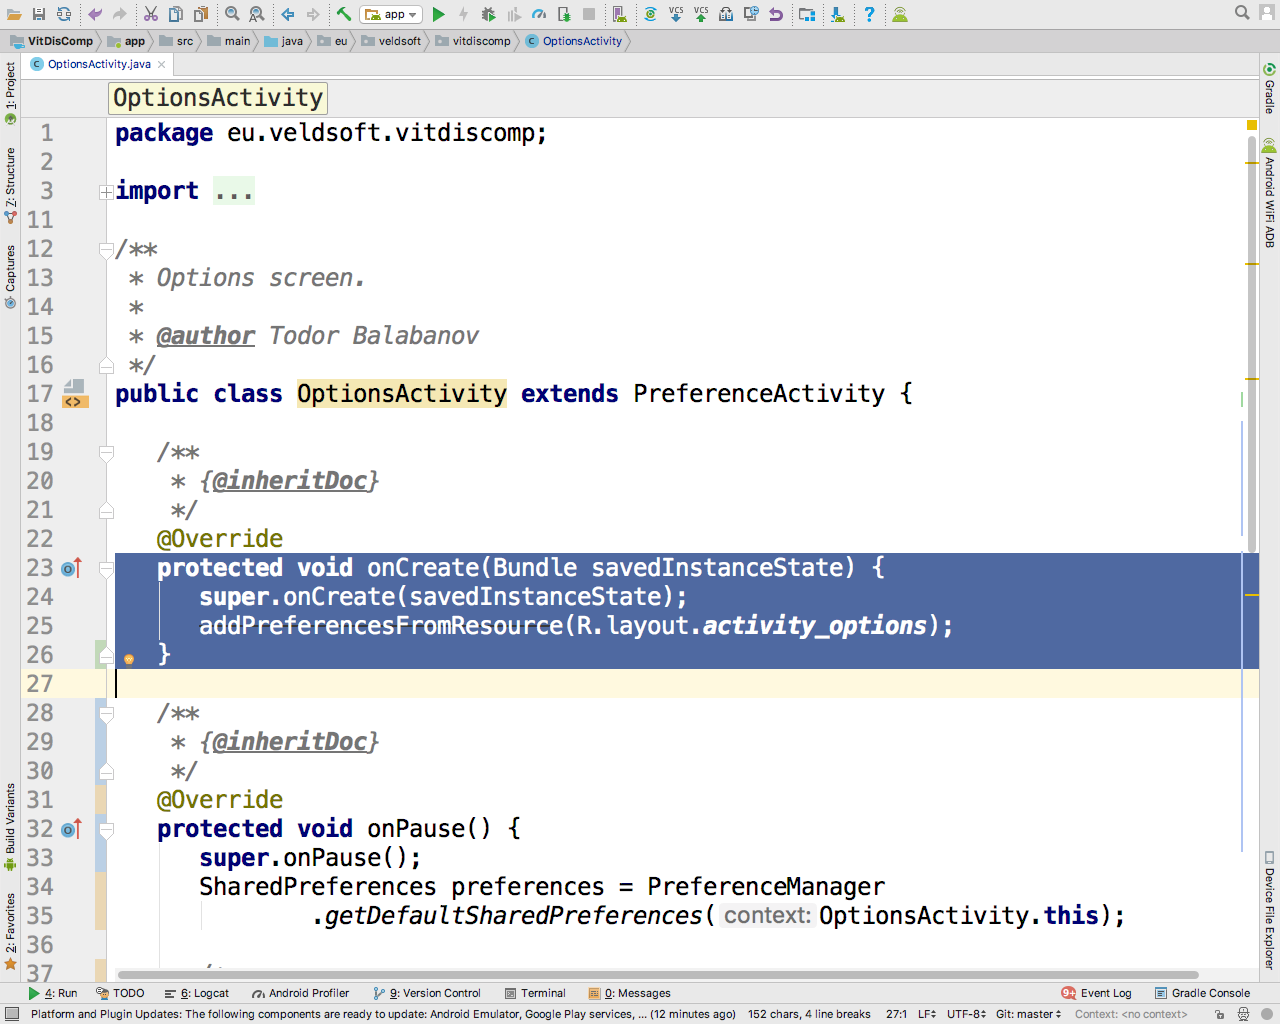
\includegraphics[height=0.45\pdfpageheight]{pic0028}
\caption{Window creation event}
\label{fig:pic0028}
\end{figure}
\FloatBarrier

The create event aims to transform the XML description of the interface into visual components visible to the user (Fig. \ref{fig:pic0028}).

\begin{figure}[h]
\centering
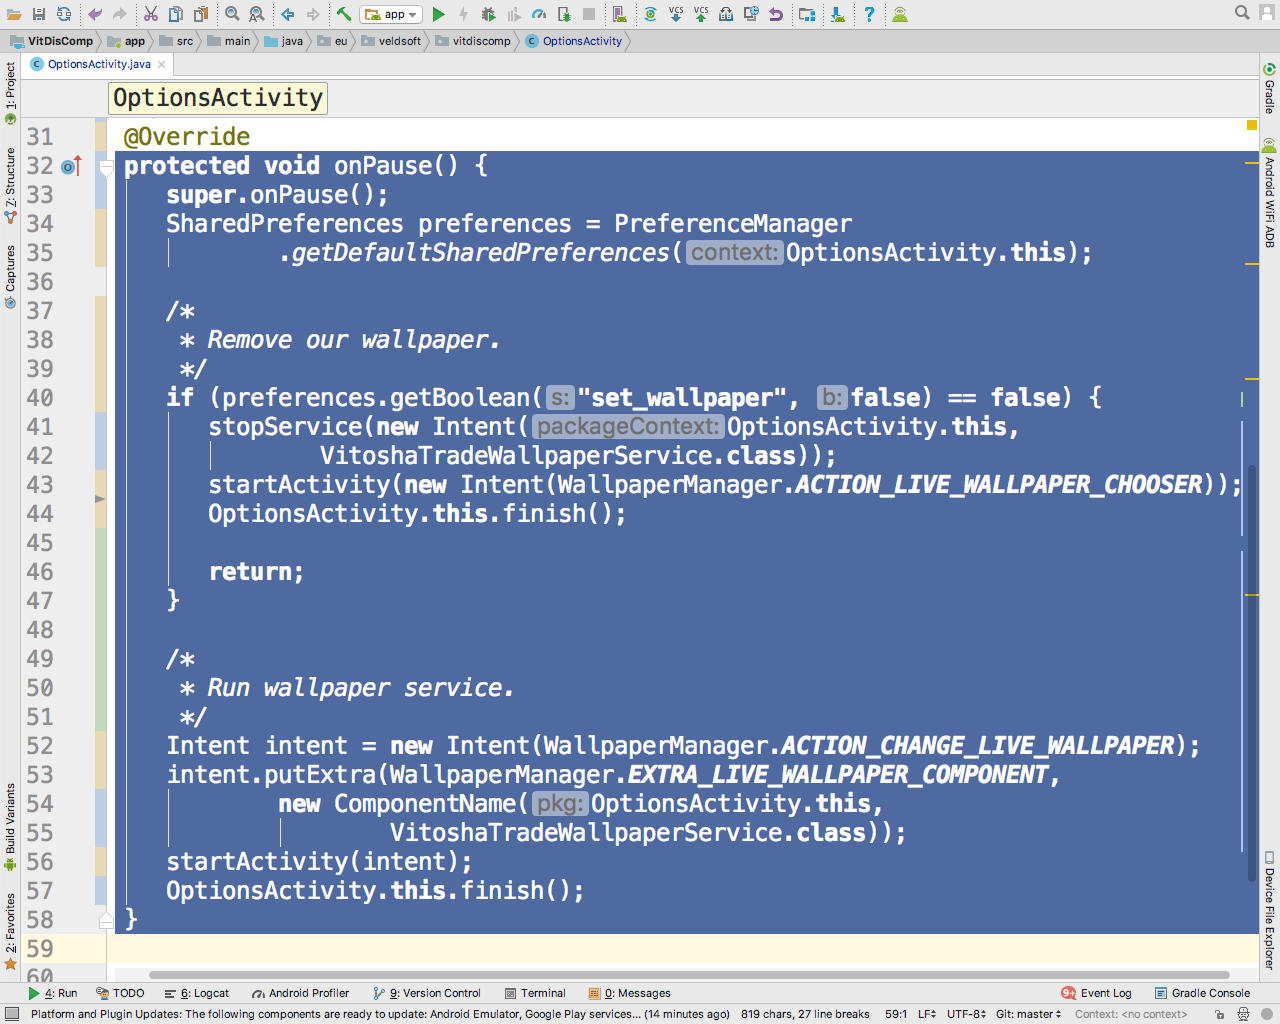
\includegraphics[height=0.45\pdfpageheight]{pic0029}
\caption{Window Pause Event}
\label{fig:pic0029}
\end{figure}
\FloatBarrier

The pause event only decides whether the active wallpaper should be started or stopped (Fig. \ref{fig:pic0029}).

\section{Background Calculation}

Long-running calculations that do not require a graphical user interface are carried out in modules called "services". When it comes to active wallpaper, it is necessary to write its class that inherits from the WallpaperService class (Fig. \ref{fig:pic0030}).

\begin{figure}[h]
\centering
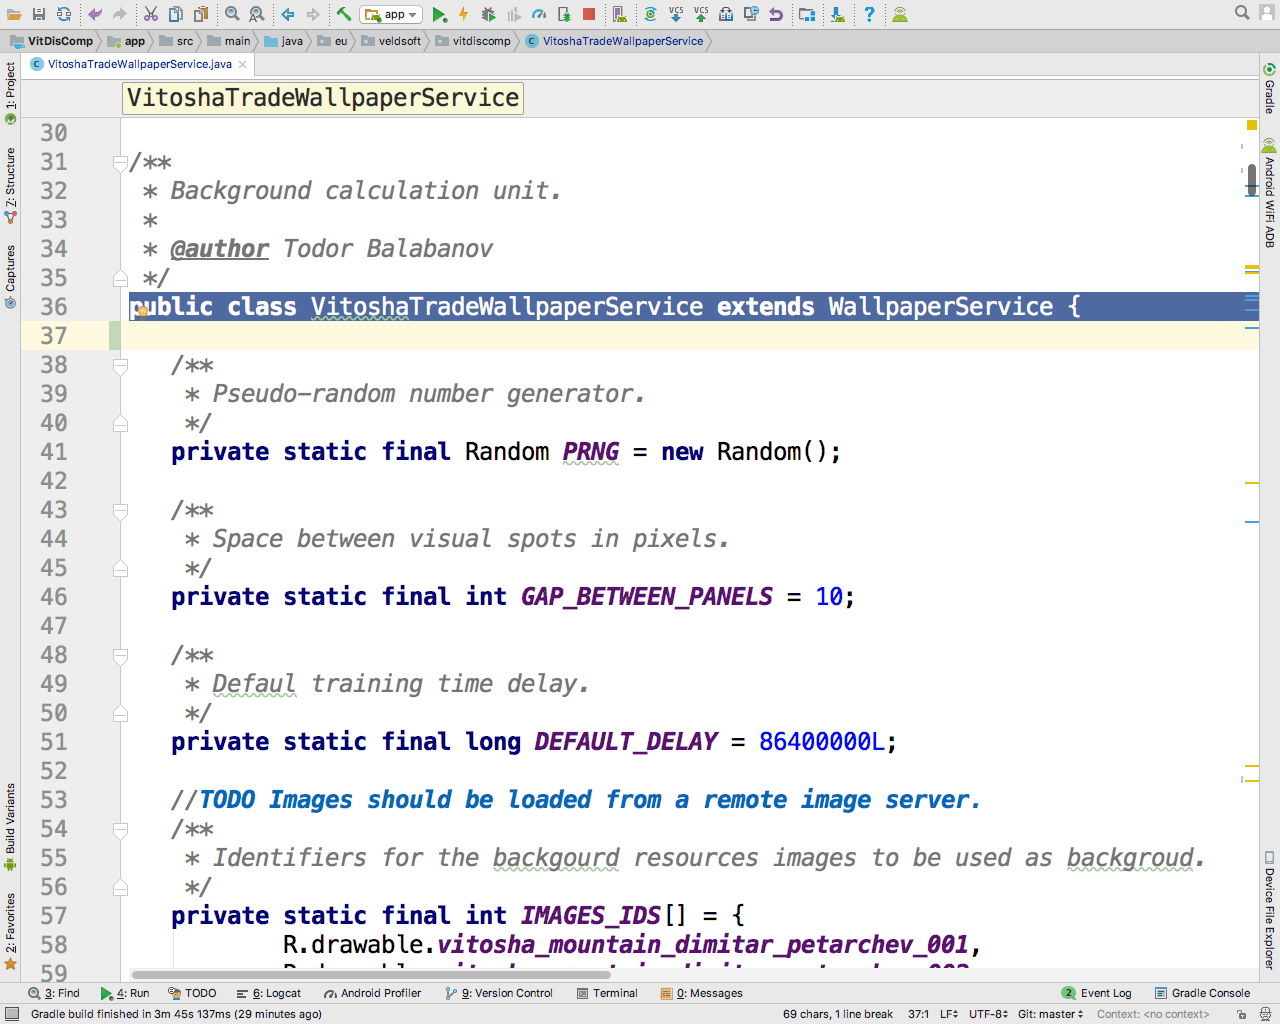
\includegraphics[height=0.45\pdfpageheight]{pic0030}
\caption{Inheriting WallpaperService}
\label{fig:pic0030}
\end{figure}
\FloatBarrier

A group of constants helps generate random numbers, specify a distance between the visual representation areas, and an implied value for the time between two separate runs of the training algorithm (Fig. \ref{fig:pic0031}).

\begin{figure}[h]
\centering
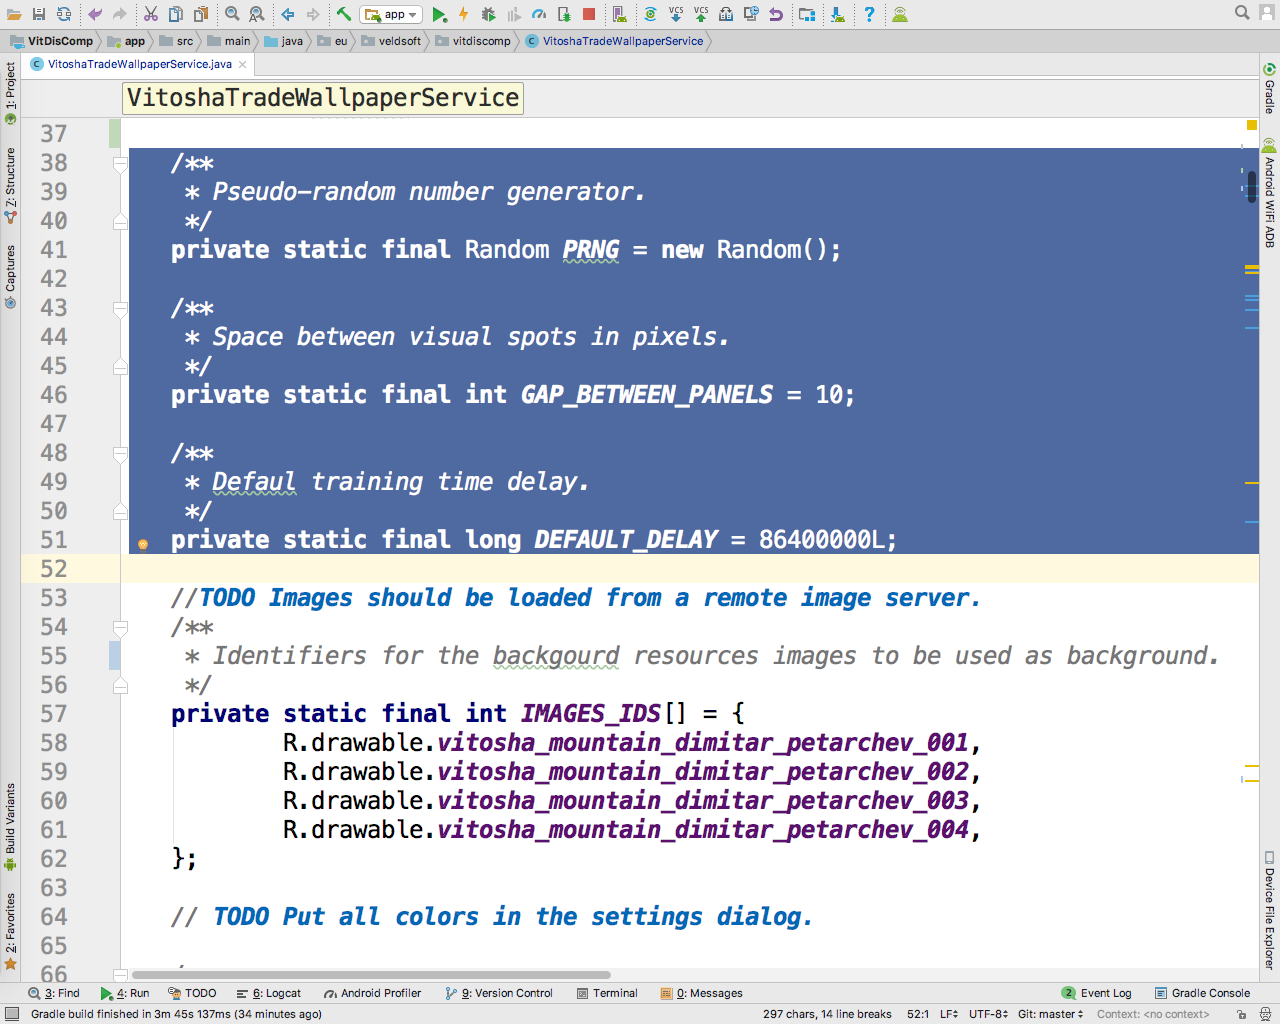
\includegraphics[height=0.45\pdfpageheight]{pic0031}
\caption{Auxiliary constants}
\label{fig:pic0031}
\end{figure}
\FloatBarrier

The colors used for the visual representation are also set with a group of constants but will subsequently be converted to settings with values from the settings window (Fig \ref{fig:pic0032}).

\begin{figure}[h]
\centering
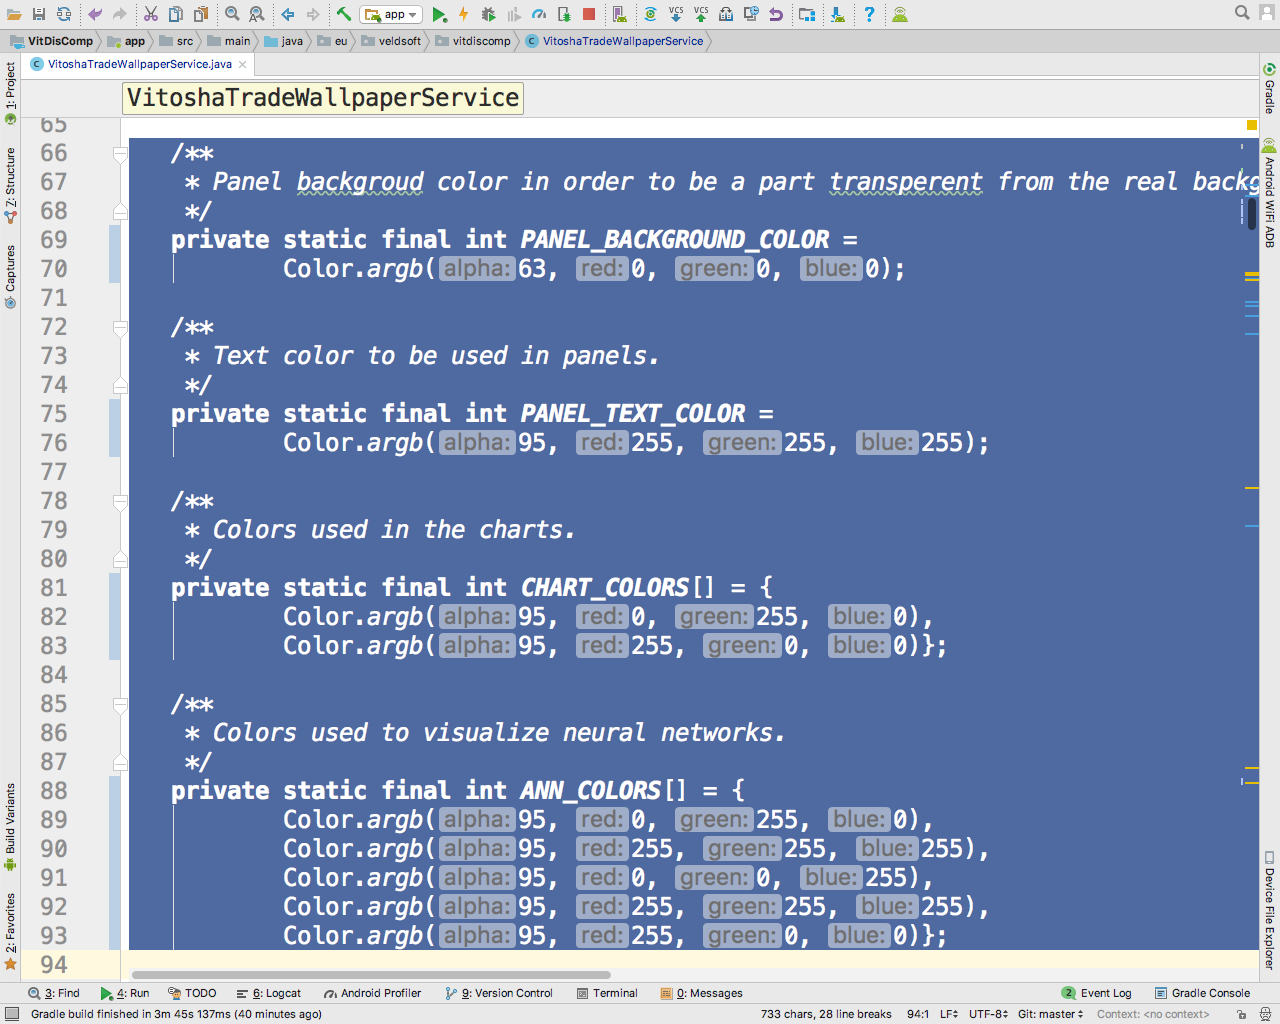
\includegraphics[height=0.45\pdfpageheight]{pic0032}
\caption{Color constants}
\label{fig:pic0032}
\end{figure}
\FloatBarrier

A group of variables is responsible for the state of the active wallpaper. This includes - screen sizes, the time between separate neural network training, whether active wallpaper is on or off, and the exact position of areas for the visual representation of information from the neural network training process (Fig. \ref{fig:pic0033}).

\begin{figure}[h]
\centering
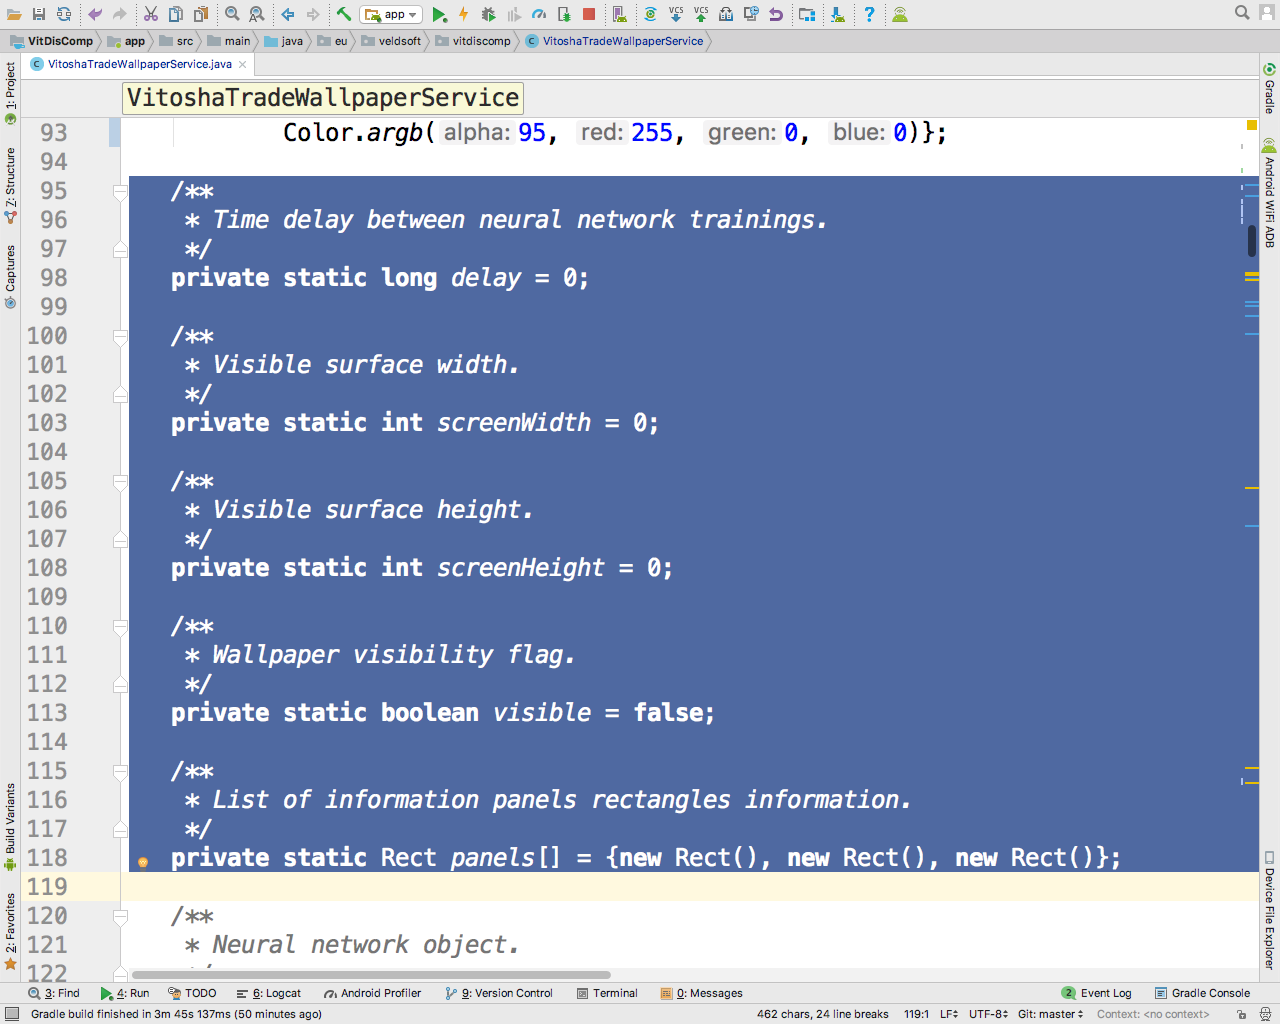
\includegraphics[height=0.45\pdfpageheight]{pic0033}
\caption{Variables reflecting the state of the active wallpaper}
\label{fig:pic0033}
\end{figure}
\FloatBarrier

Another group of variables (references to objects) takes responsibility for managing the artificial neural network, the training examples, the input-output data to the network, and the rule for its training (Fig. \ref{fig:pic0034}).

\begin{figure}[h]
\centering
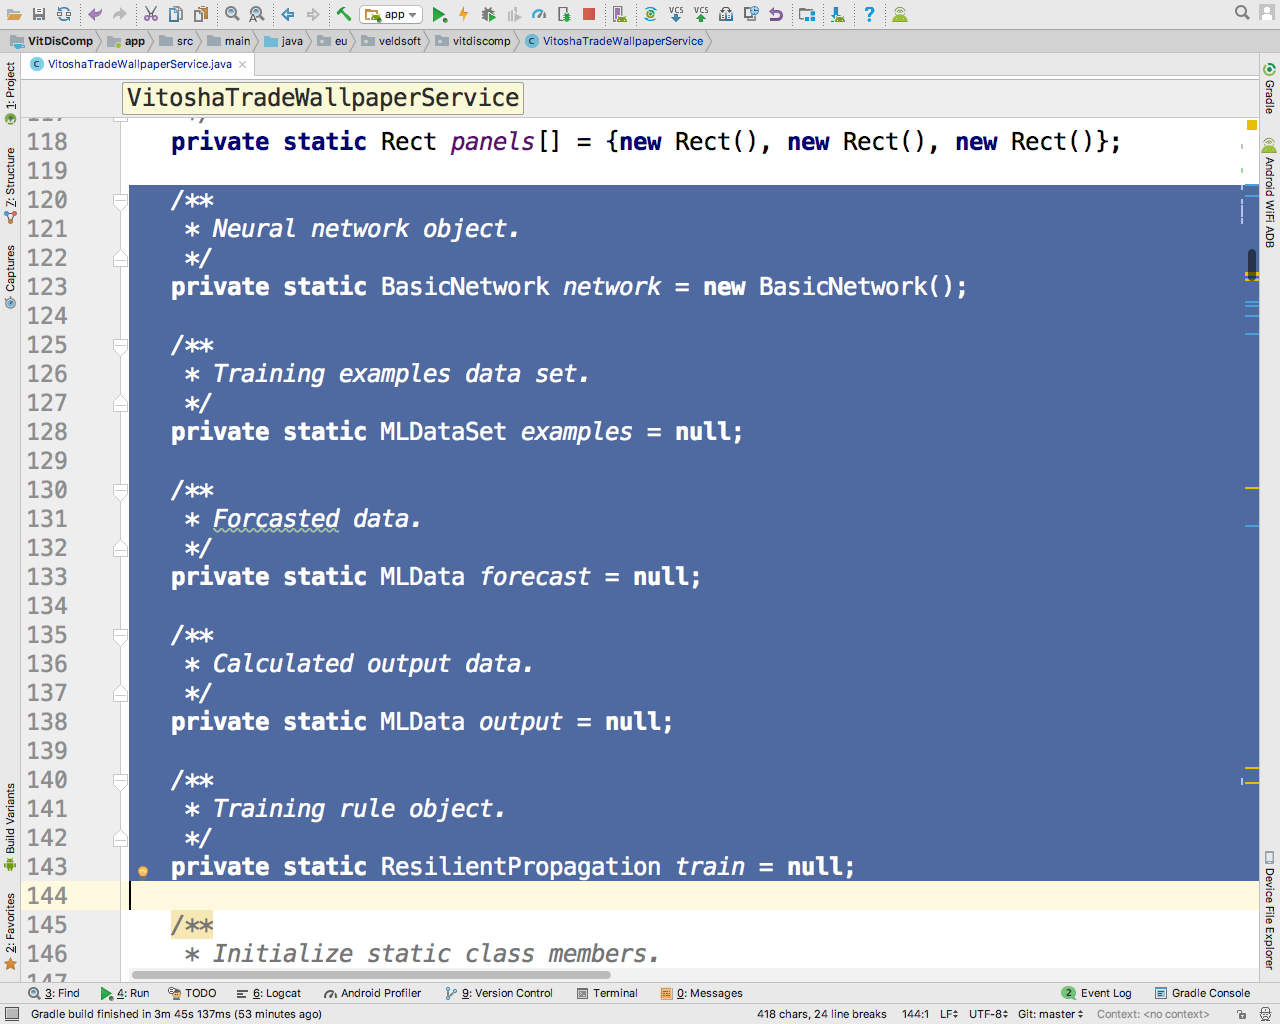
\includegraphics[height=0.45\pdfpageheight]{pic0034}
\caption{Variables responsible for artificial neural network}
\label{fig:pic0034}
\end{figure}
\FloatBarrier

In commercial software production, a widespread trick is to create "software plugs". These are pieces of code that communicate between objects and parts of the system that still need to be made. In the present case, just such a software plug represents the absence of a server and a real data source (Fig. \ref{fig:pic0035}).

\begin{figure}[h]
\centering
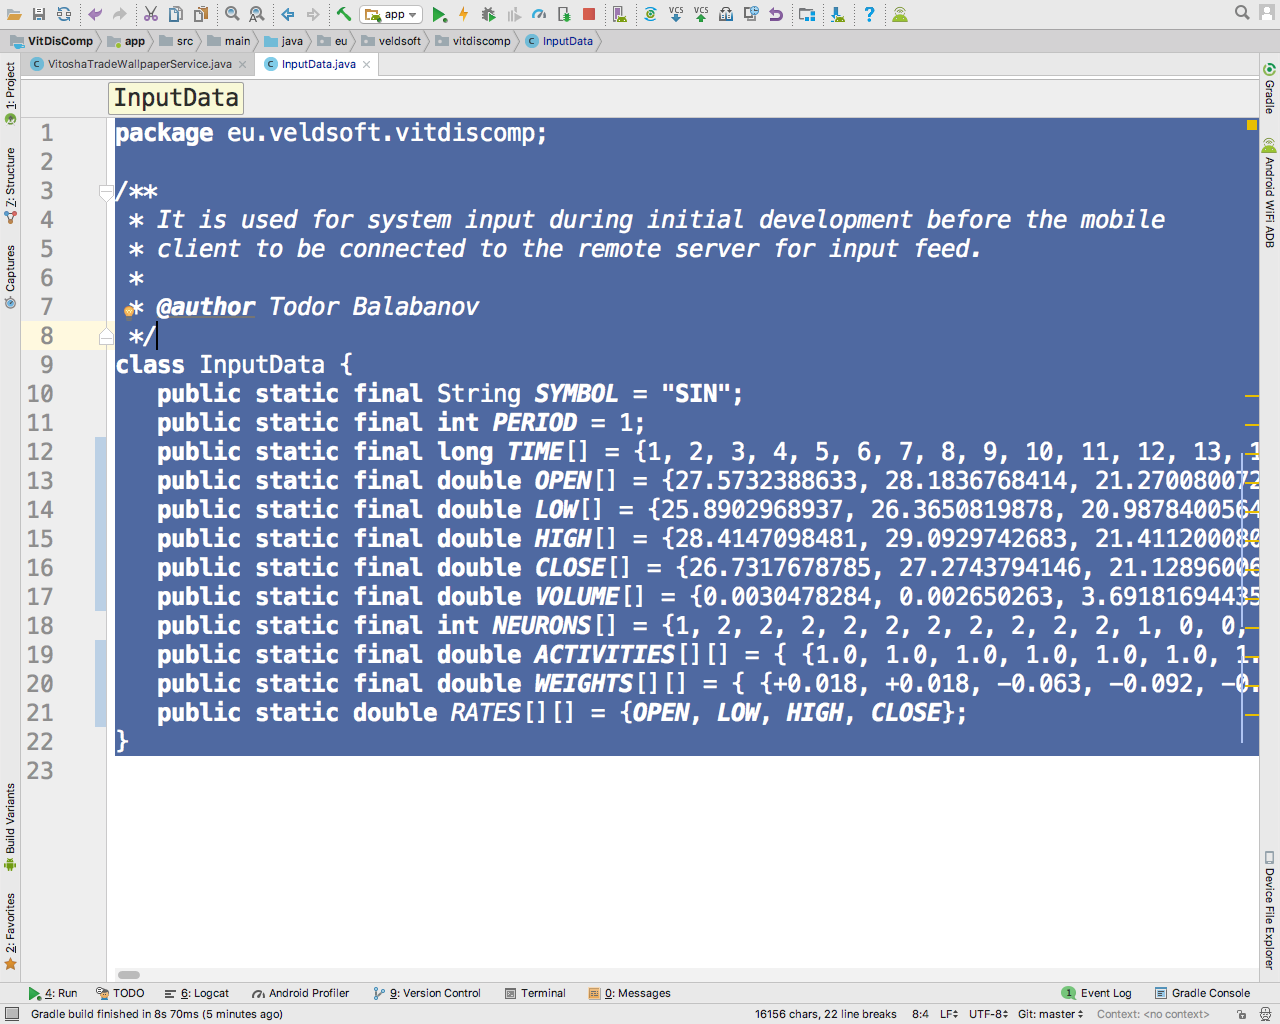
\includegraphics[height=0.45\pdfpageheight]{pic0035}
\caption{Variables responsible for artificial neural network}
\label{fig:pic0035}
\end{figure}
\FloatBarrier

Financial time series are often described with the following characteristics: 1. Type of financial instrument (ticker symbol or stock symbol), in this case, the mathematical function sine; 2. The interval between individual measurements (counted in minutes), in this case, one minute; 3. Six parallel arrays (discrete time, open levels, lowest level reached, the highest level reached, close levels, and volume traded).

In addition to financial information, information about the topology of the artificial neural network must also be submitted to the client application. The description of the artificial neural network requires: 1. Number, arrangement, and type of neurons (a one-dimensional array of constants); 2. Adjacency matrix between neurons (one where there is a connection and zero where there is no connection); 3. The current value of the weight coefficient for each connection between two neurons (including loops, if any).

\begin{figure}[h]
\centering
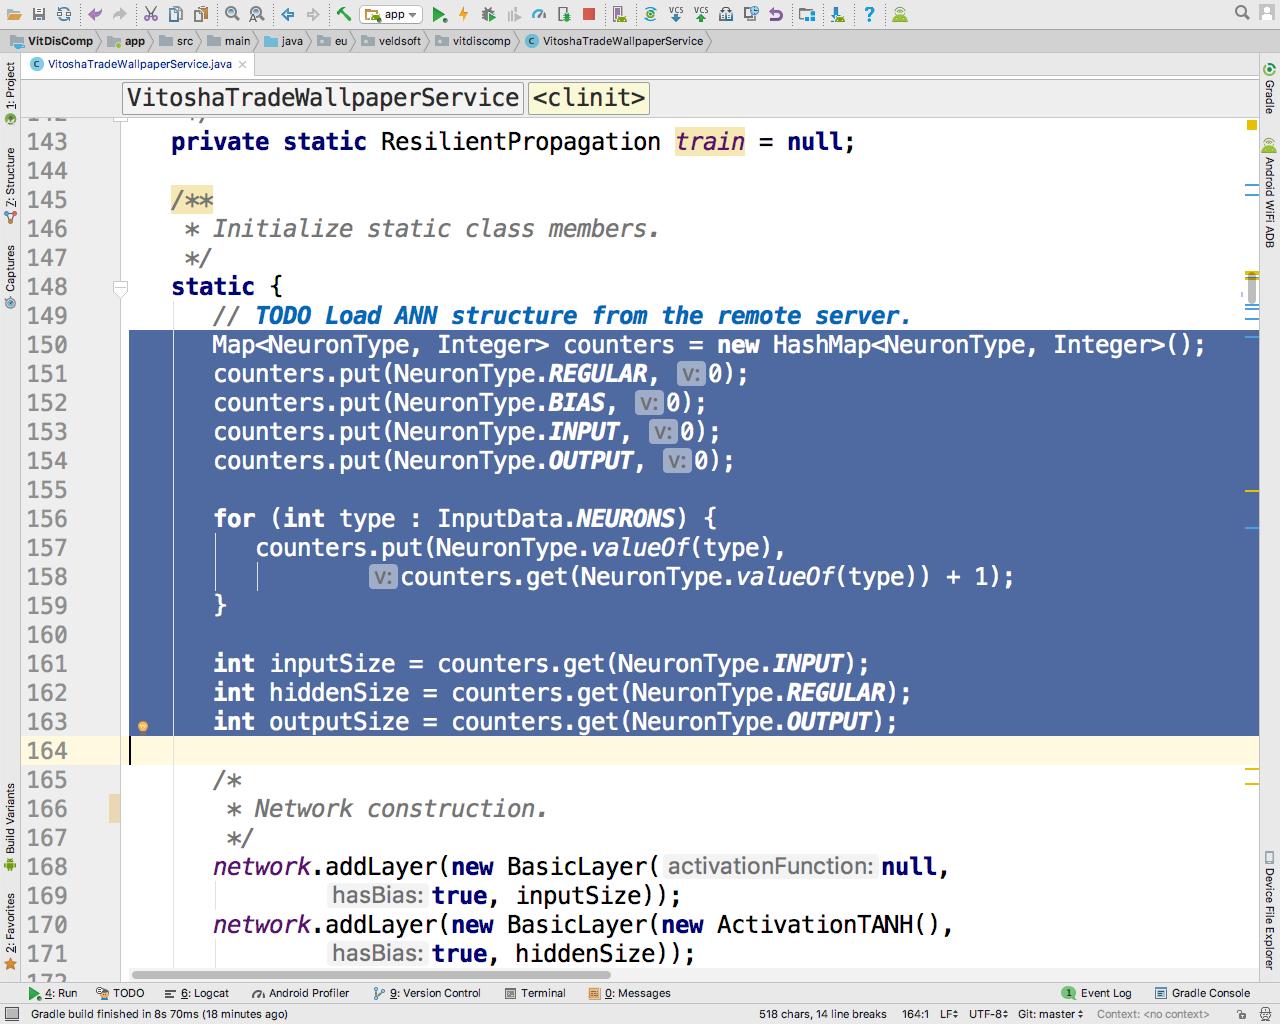
\includegraphics[height=0.45\pdfpageheight]{pic0036}
\caption{Determining the number and types of neurons}
\label{fig:pic0036}
\end{figure}
\FloatBarrier

Counting sorting efficiently determines the number of neurons and their types (Fig. \ref{fig:pic0036}).

\begin{figure}[h]
\centering
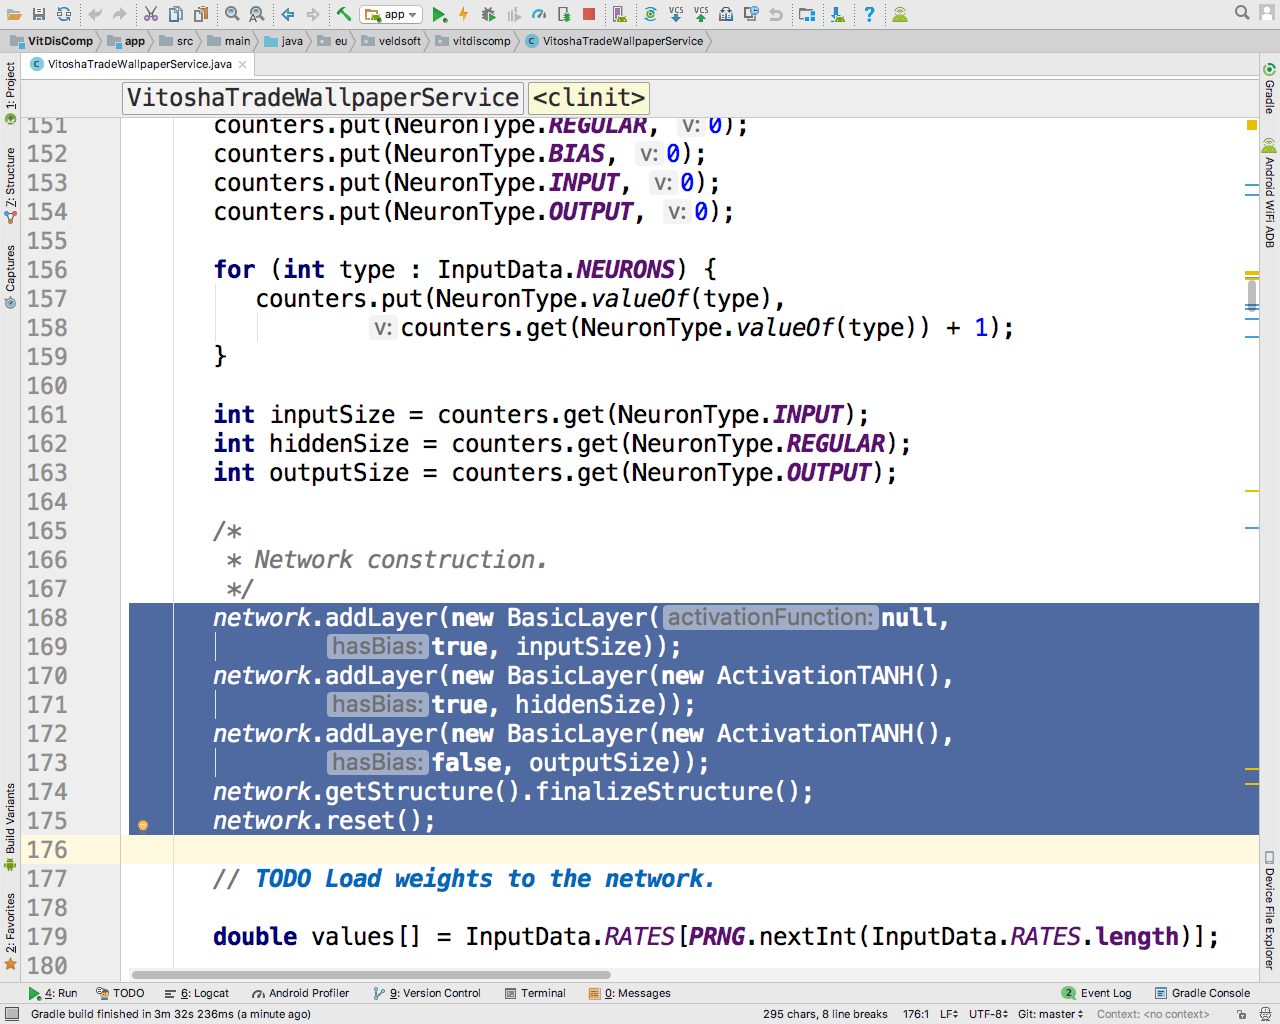
\includegraphics[height=0.45\pdfpageheight]{pic0037}
\caption{Structure of a three-layer artificial neural network}
\label{fig:pic0037}
\end{figure}
\FloatBarrier

To illustrate the predictive capabilities of artificial neural networks, one of the most used topologies is chosen, namely a three-layer neural network that is trained with error backpropagation (Fig. \ref{fig:pic0037}). The input layer has the sole task of receiving the signals from the external environment, so no activation function is set. The function $\tanh( x )$ (hyperbolic tangent) is chosen for the hidden and output layers since it is asymptotically convergent at infinity along the abscissa and, simultaneously, is symmetric along this same axis. Training is slightly faster with a hyperbolic tangent because the signal values in the hidden layers are more easily "skewed" in a positive or negative direction. In comparison, with the sigmoid function, the signals are only positive; if negative values are needed, this compensation must be obtained only through negative link weights. The input and hidden layers have a bias neuron that is not required in the output layer because the bias neuron constantly emits the high-level signal.

\begin{figure}[h]
\centering
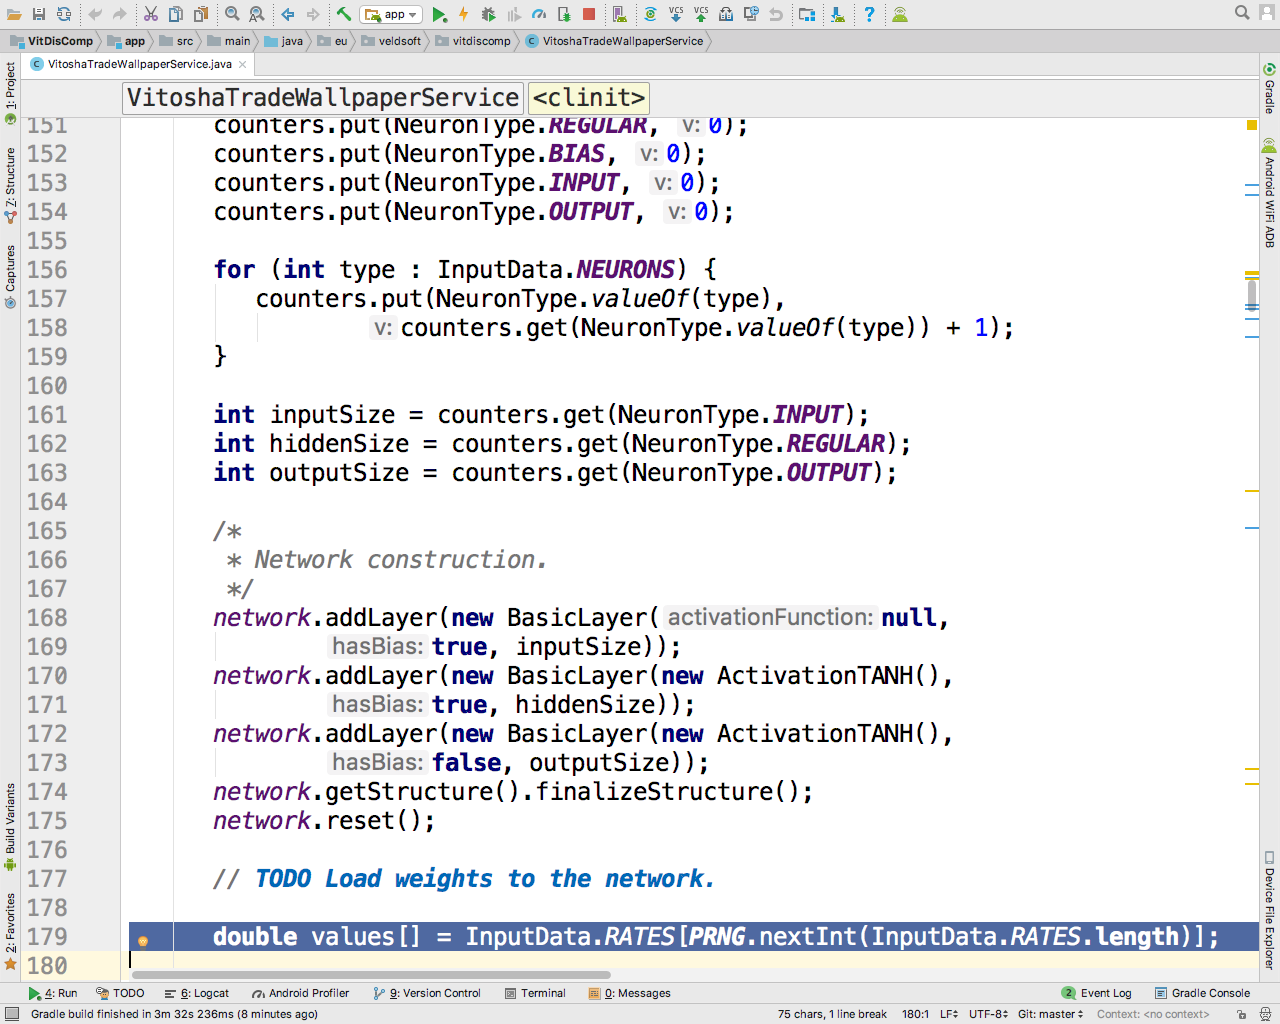
\includegraphics[height=0.45\pdfpageheight]{pic0038}
\caption{Choosing values to predict}
\label{fig:pic0038}
\end{figure}
\FloatBarrier

From the description of parallel arrays in financial time series, it is clear that there are four possible sequences of numbers to feed to the neural network for prediction (open, low, high, and close).

\begin{figure}[h]
\centering
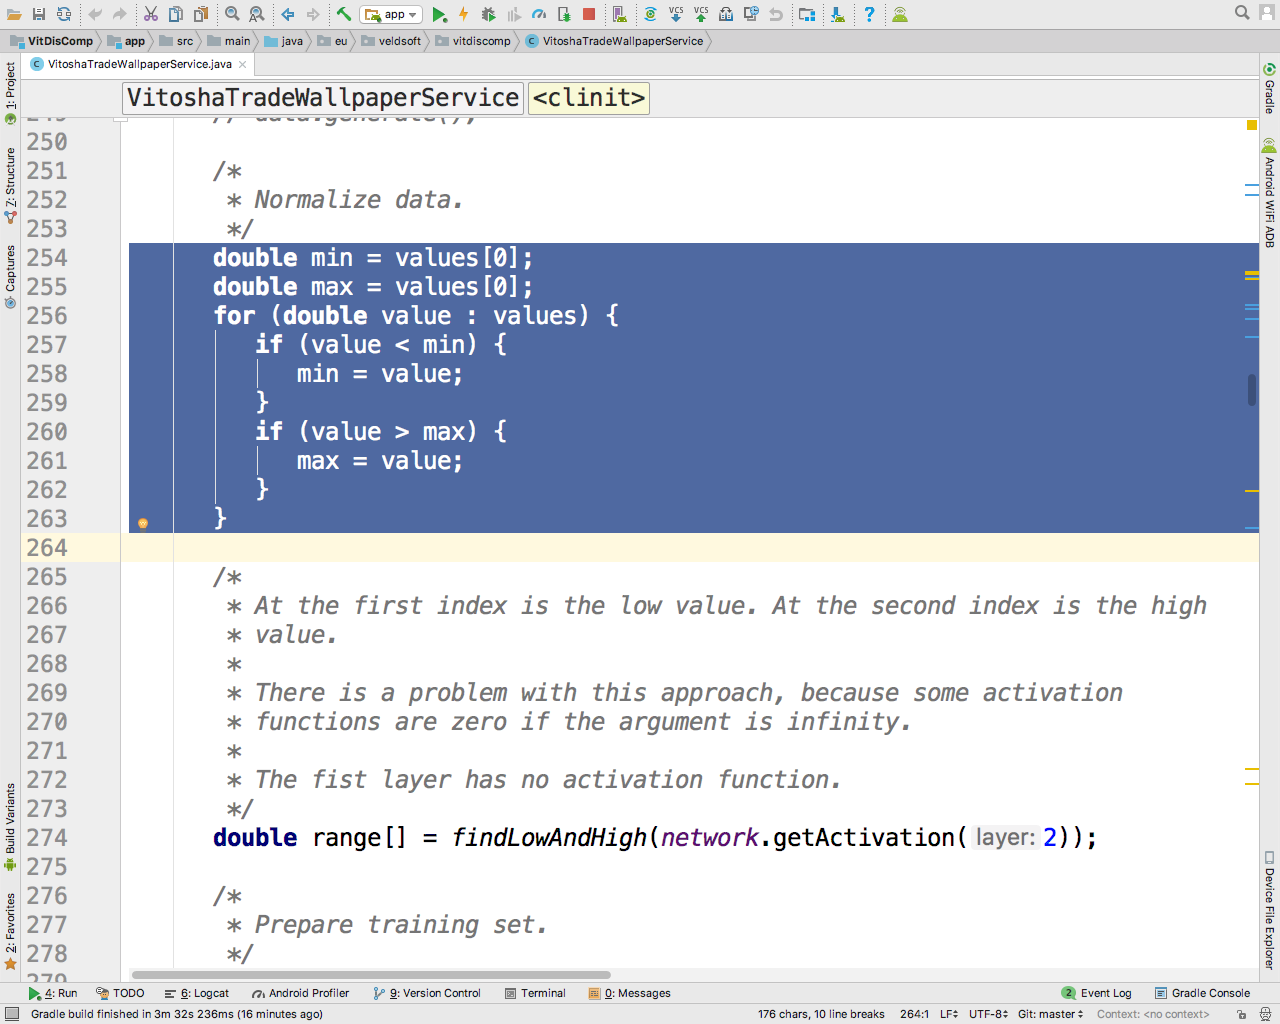
\includegraphics[height=0.45\pdfpageheight]{pic0039}
\caption{Determining boundaries in the time series}
\label{fig:pic0039}
\end{figure}
\FloatBarrier

In practice, the closing value series is most often used, and the purpose is to predict the opening level in the next time interval. The objectives of this presentation are not to achieve financial predictions, and for this reason, it is a randomly chosen sequence to use in the different training/forecasting runs (Fig. \ref{fig:pic0038}).

\begin{figure}[h]
\centering
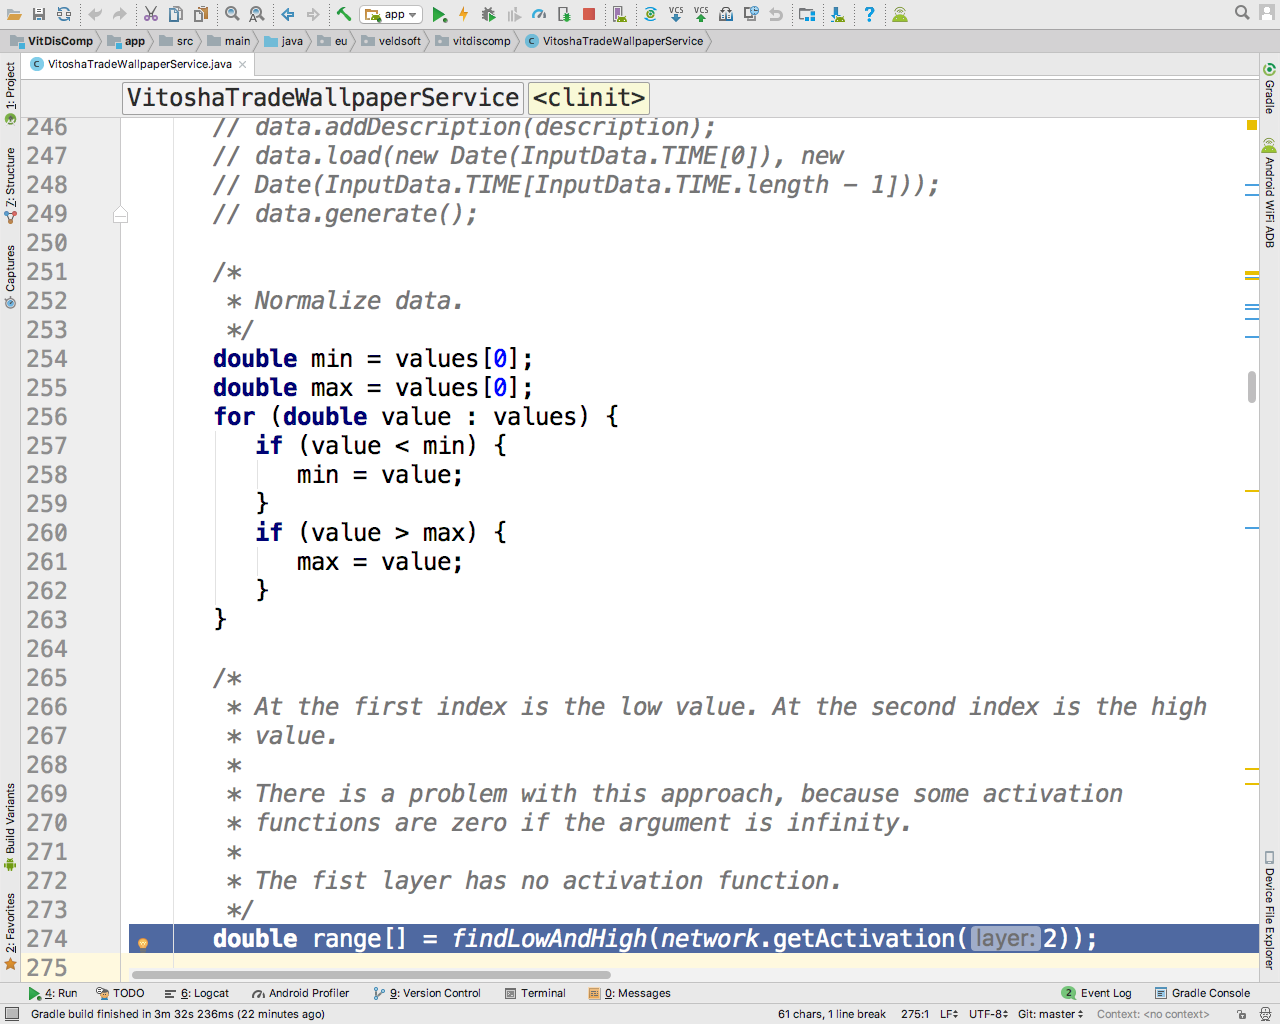
\includegraphics[height=0.45\pdfpageheight]{pic0040}
\caption{Range of the activation function in the output layer}
\label{fig:pic0040}
\end{figure}
\FloatBarrier

Since the goal is to feed different financial time series to the forecasting system, the input information in the system inevitably needs to be pre-normalized, and the first step to this is to determine the most significant and most minor values in the time series ( Fig. \ref{fig:pic0039}). At the same time, the data must be matched to the range in which the activation functions of the artificial neural network work. This tutorial assumes that signals in the scope of the function used in the output layer will be applied to the input (Fig. \ref{fig:pic0040}). This decision is explained by the fact that the information fed by the neural network to the external environment will undergo a reverse resizing process to make sense of the particular financial time series.

\begin{figure}[h]
\centering
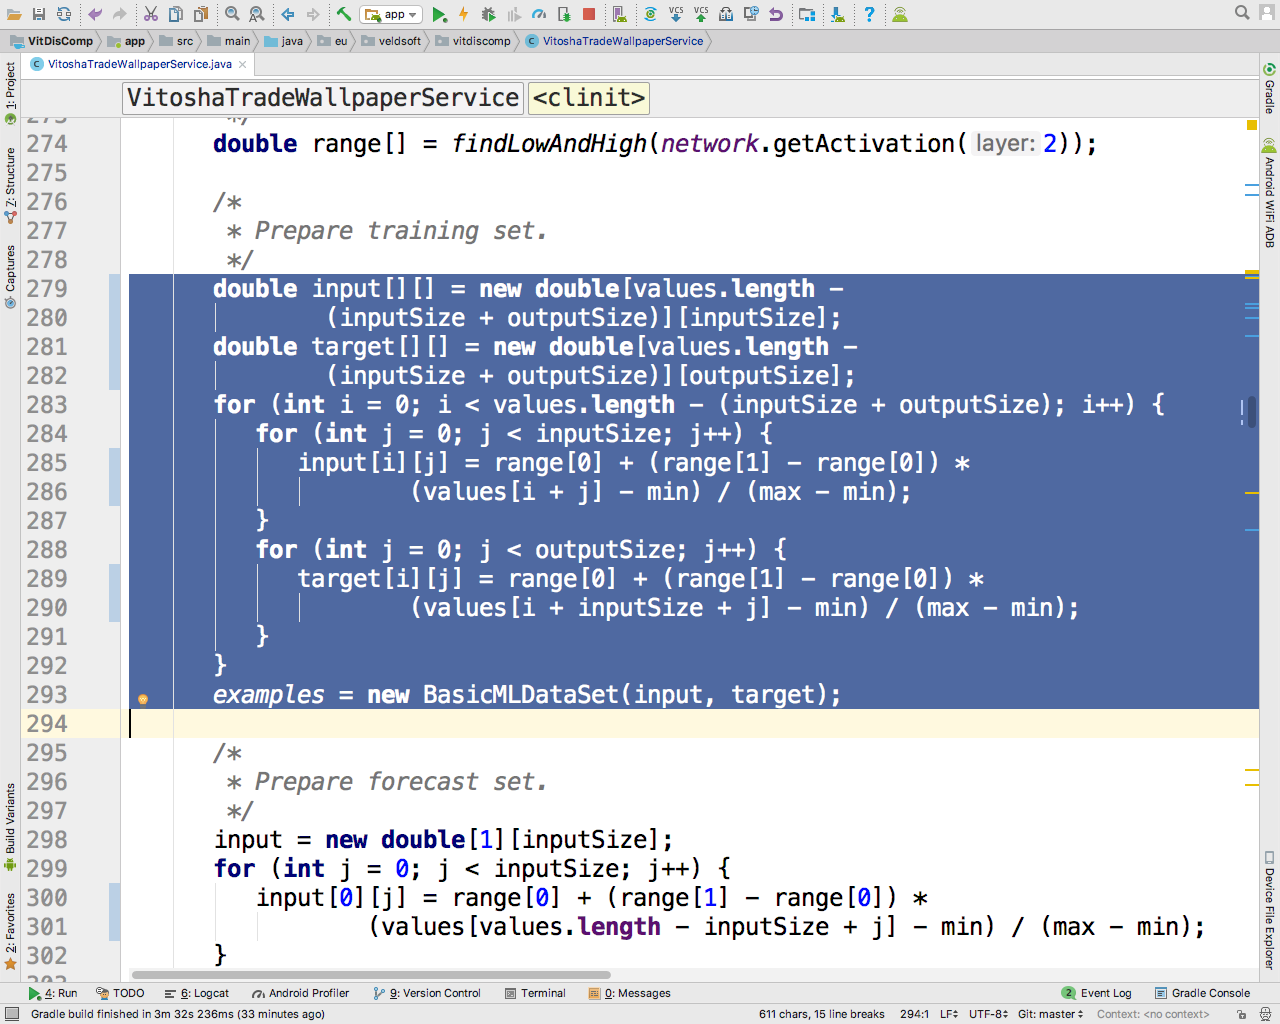
\includegraphics[height=0.45\pdfpageheight]{pic0041}
\caption{Training examples}
\label{fig:pic0041}
\end{figure}
\FloatBarrier

We conditionally divide the normalized input data into two sets (measurements in the past and measures in the future). The separation is conditional since practically the data are from real measurements in the past (Fig. \ref{fig:pic0041}).

\begin{figure}[h]
\centering
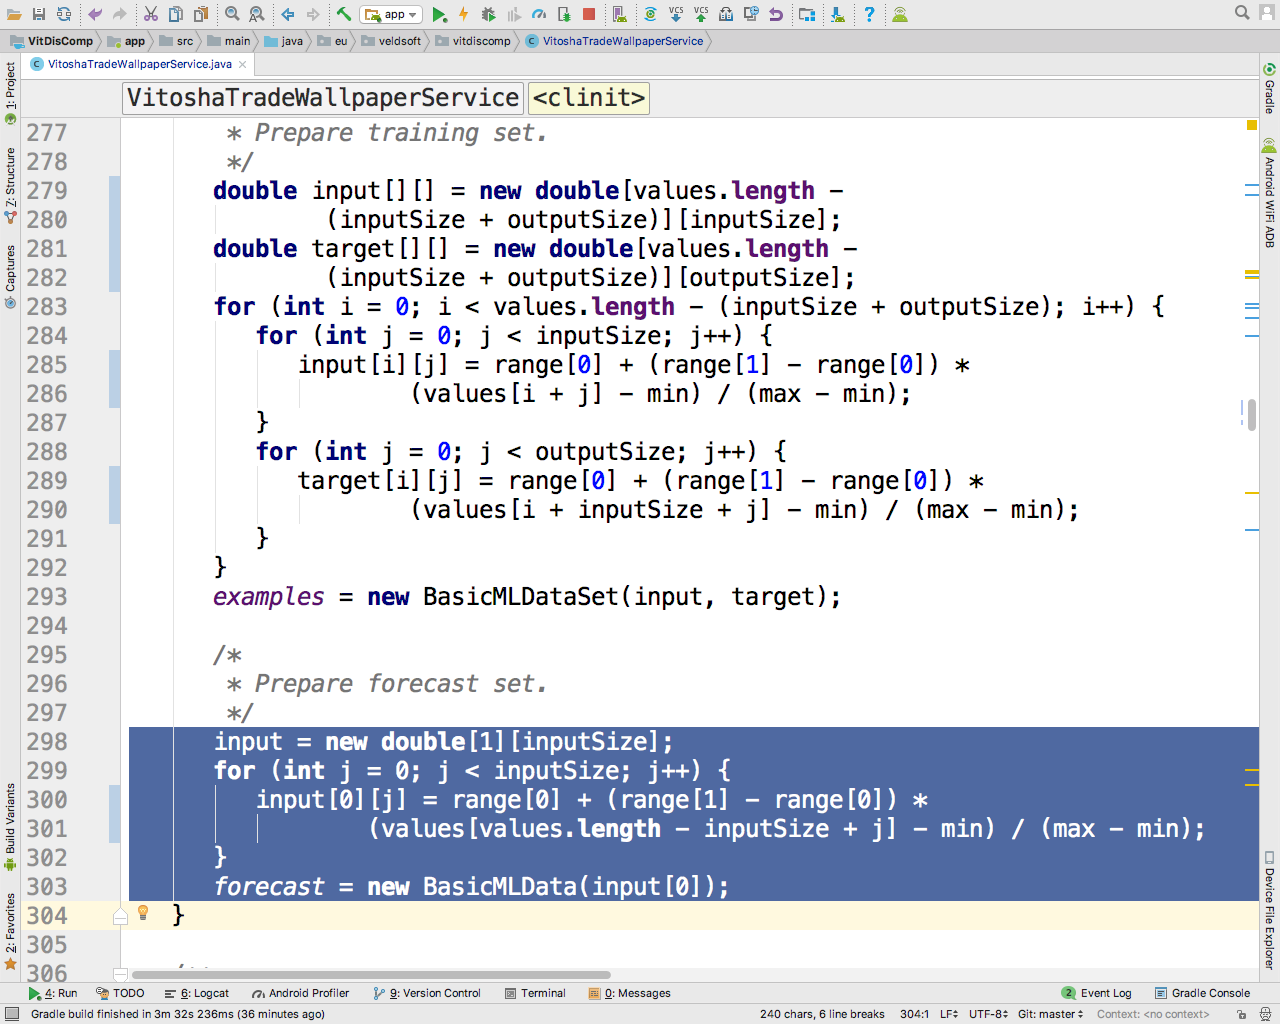
\includegraphics[height=0.45\pdfpageheight]{pic0042}
\caption{Input to the artificial neural network to obtain a prediction}
\label{fig:pic0042}
\end{figure}
\FloatBarrier

Since the artificial neural network is used in both its modes (training and prediction), it also prepares a vector of input data against which to make a prediction (Fig. \ref{fig:pic0042}).

\begin{figure}[h]
\centering
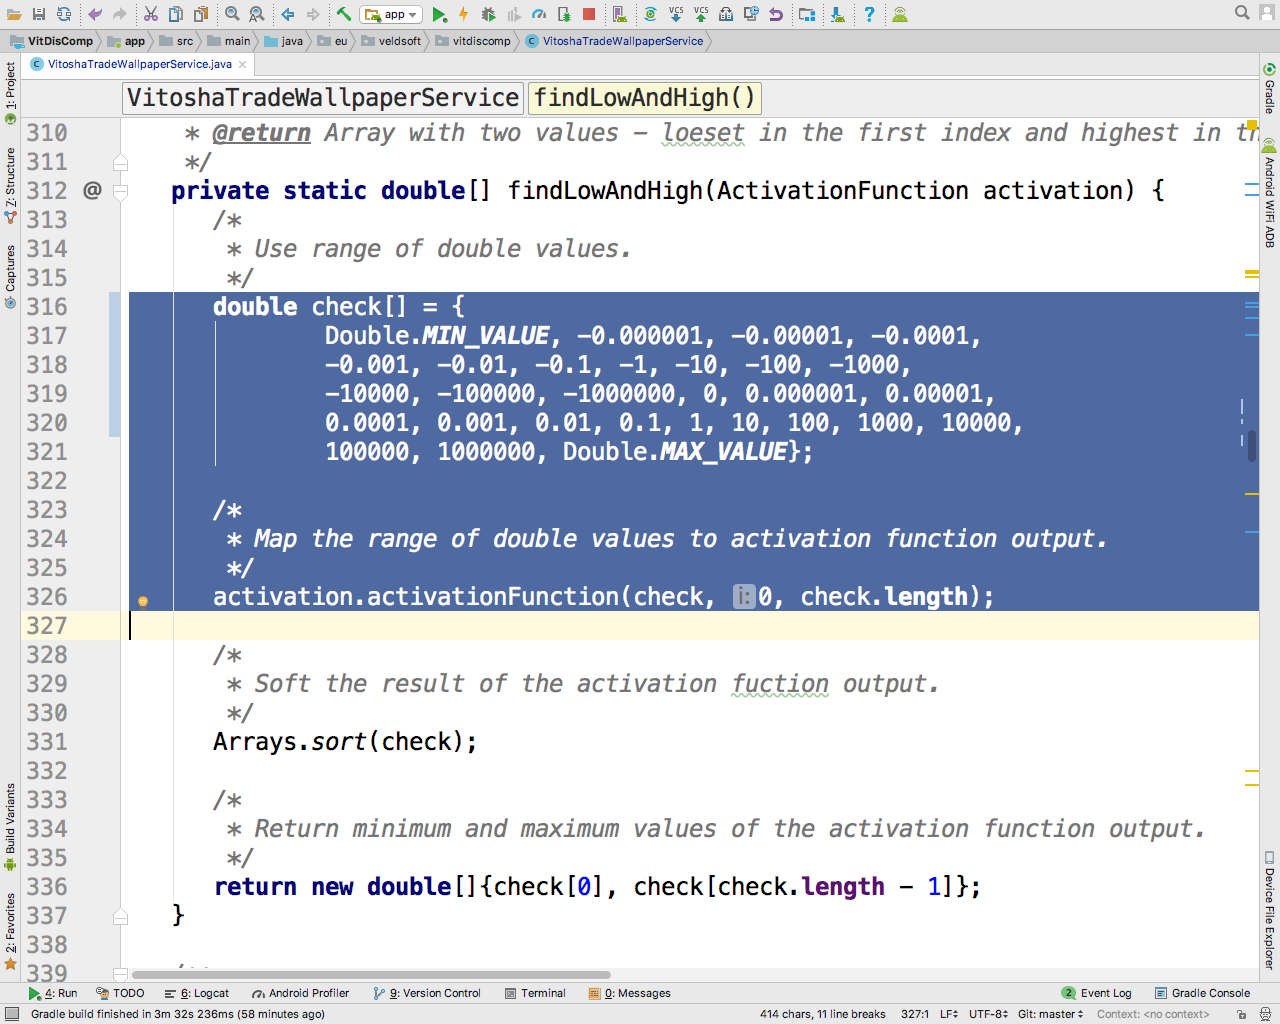
\includegraphics[height=0.45\pdfpageheight]{pic0043}
\caption{Exploring a group of values to determine the range}
\label{fig:pic0043}
\end{figure}
\FloatBarrier

In general, the activation functions have asymptotic convergence and are monotonically increasing (Fig. \ref{fig:pic0044}), which allows their finite ranges to be established by inspecting a set of values (Fig. \ref{fig:pic0043}).

\begin{figure}[h]
\centering
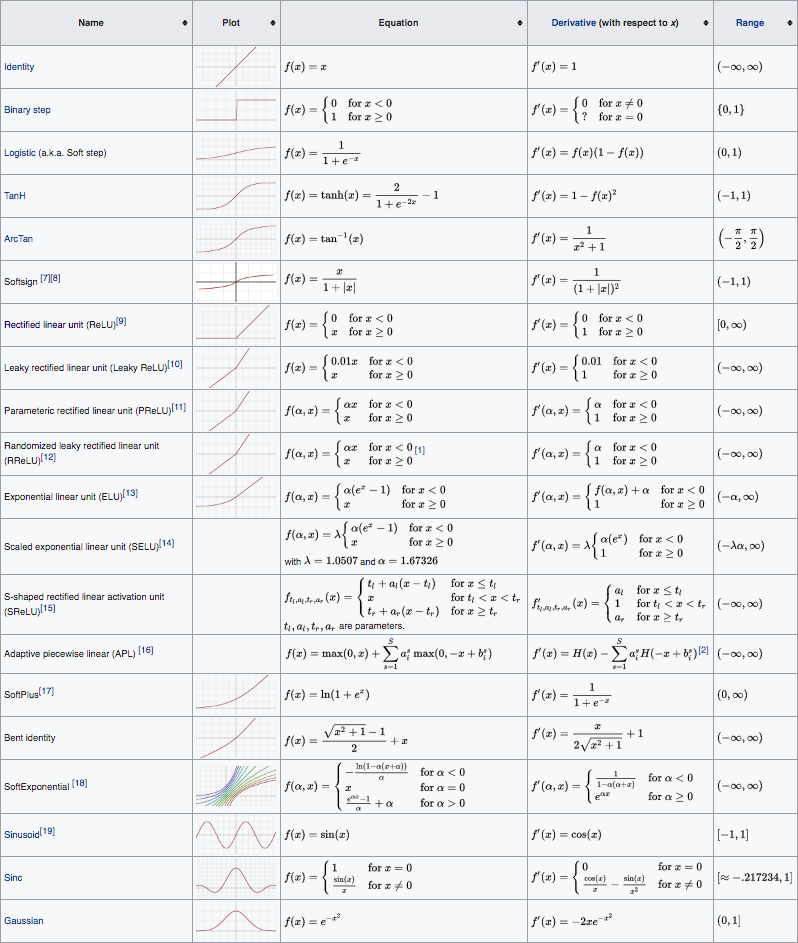
\includegraphics[height=0.7\pdfpageheight]{pic0044}
\caption{Activation Functions \cite{afwiki}}
\label{fig:pic0044}
\end{figure}
\FloatBarrier

As is visible in Fig. \ref{fig:pic0044}, for some of the activation functions, such a range determination can be highly misleading (e.g., the sine function).

\begin{figure}[h]
\centering
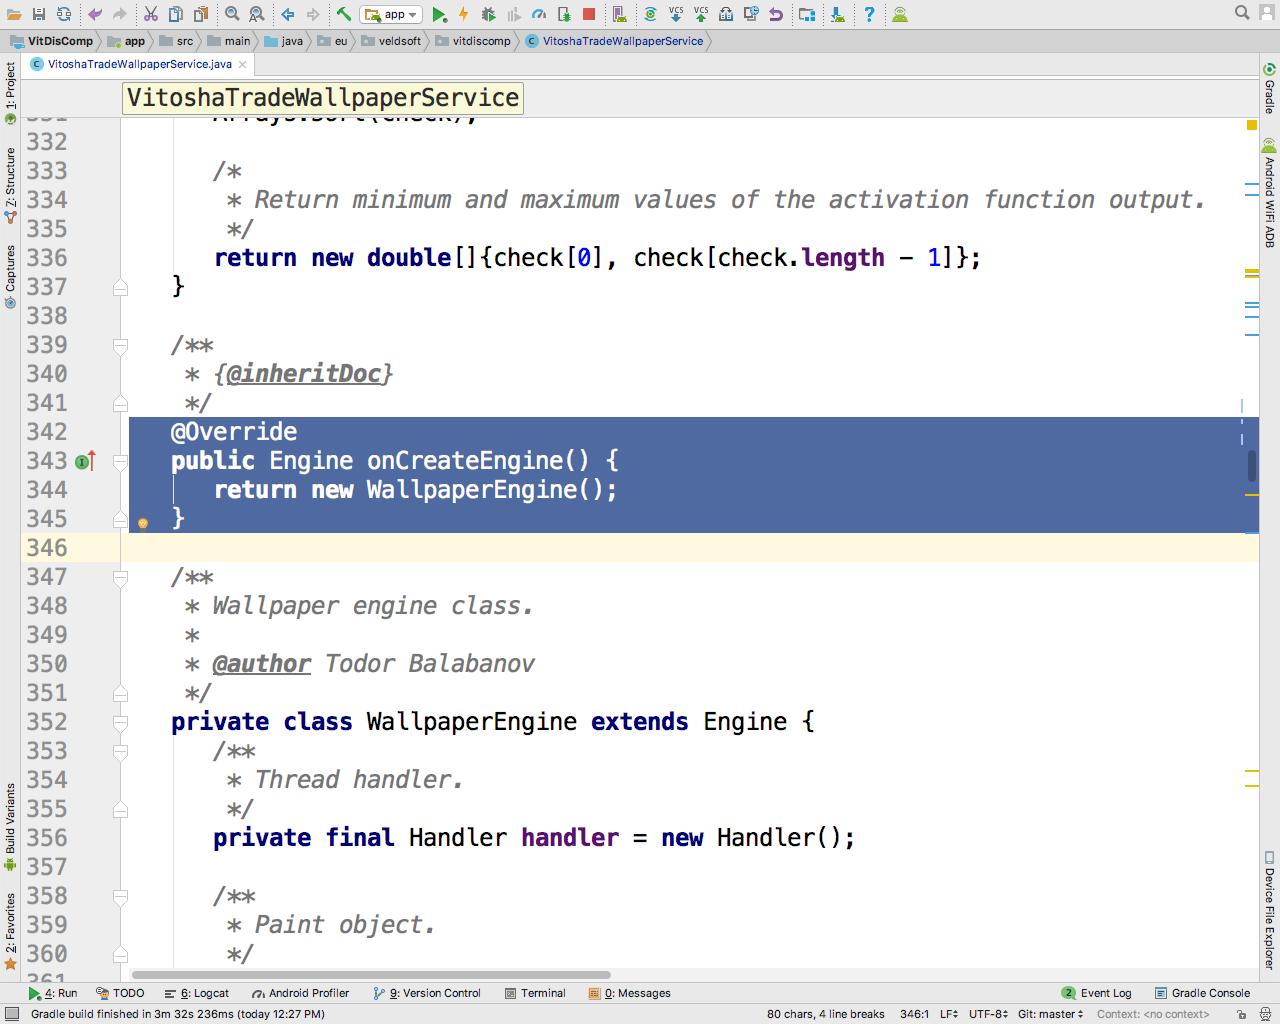
\includegraphics[height=0.45\pdfpageheight]{pic0045}
\caption{Custom implementation of the inherited Engine class and object creation}
\label{fig:pic0045}
\end{figure}
\FloatBarrier

The engine object creation event is redefined to return an object from our engine class (Fig \ref{fig:pic0045}).

\section{Service Engine}

The actual background computation work in the service is done by an object described by a private inner class of type "Engine".

\begin{figure}[h]
\centering
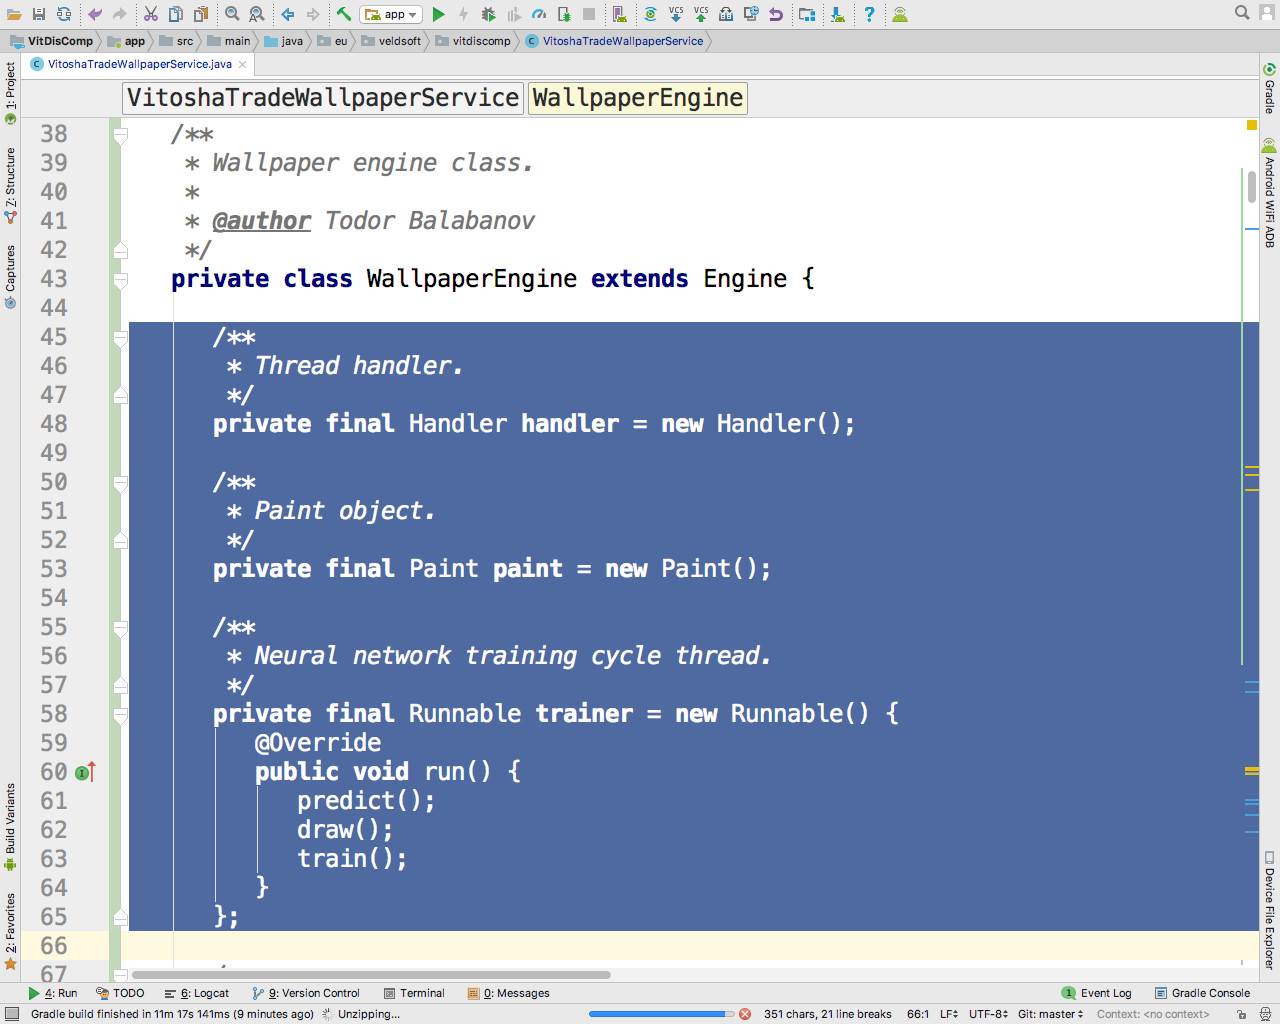
\includegraphics[height=0.45\pdfpageheight]{pic0046}
\caption{Internal variables for the service engine}
\label{fig:pic0046}
\end{figure}
\FloatBarrier

Three internal variables are used in this engine (Fig \ref{fig:pic0046}). The object of type "brush" (Paint) is only auxiliary and serves to define the characteristics of painting once. The benefit is that the object is created once and then used throughout the service's life cycle.

\begin{figure}[h]
\centering
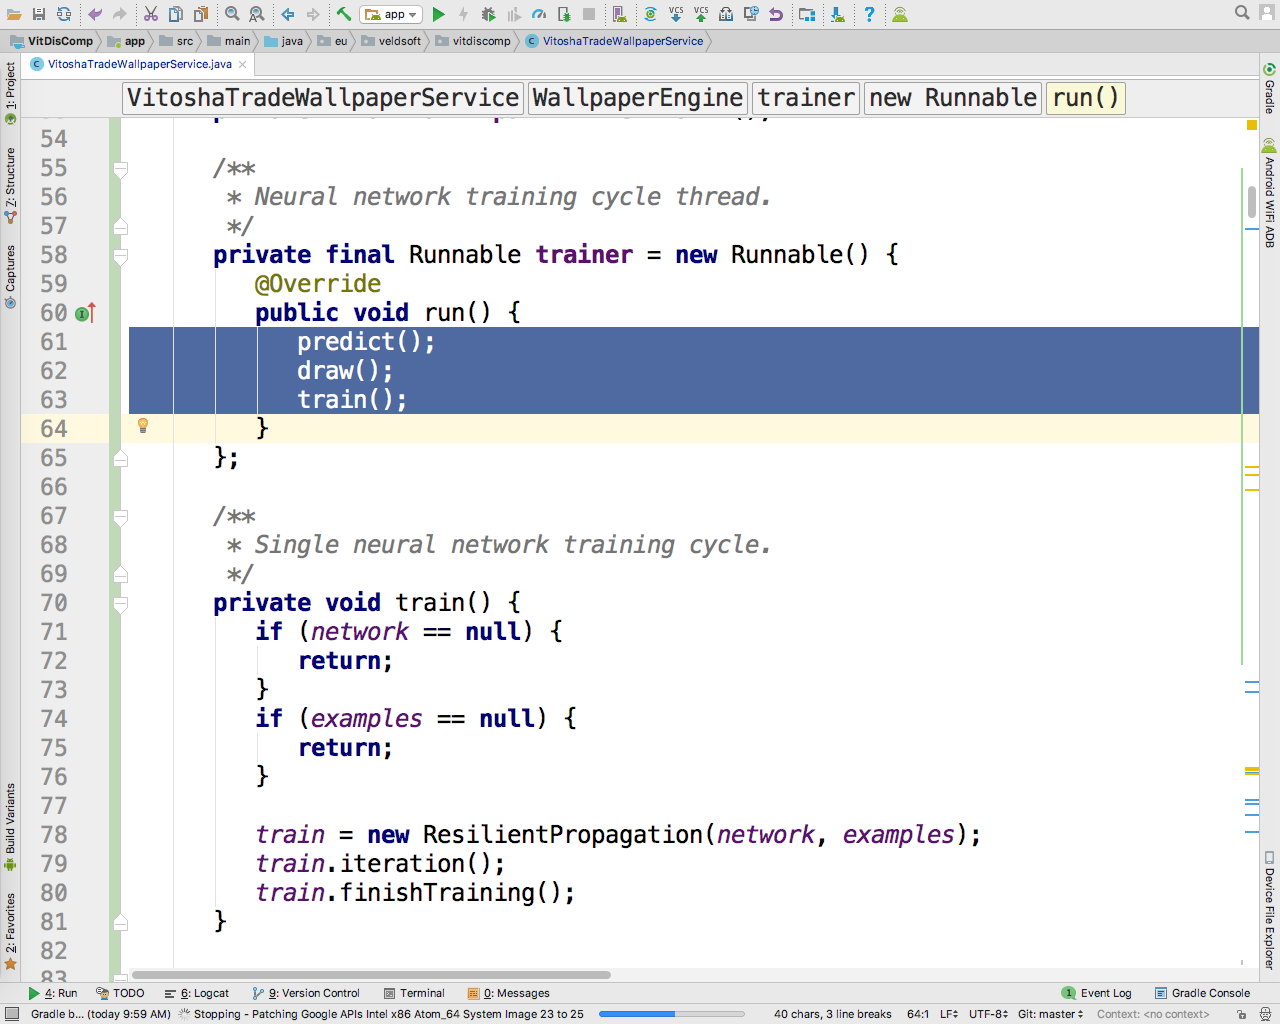
\includegraphics[height=0.45\pdfpageheight]{pic0047}
\caption{Single loop in background}
\label{fig:pic0047}
\end{figure}
\FloatBarrier

For the actual operation of the engine, a separate thread (trainer) is defined to perform the operations of generating a prediction, drawing the active wallpaper, and completing one cycle of the training process of the artificial neural network\index{artificial neural networks} (Fig. \ref {fig:pic0047}). Effective thread management in Android is done using Handler objects. The Handler object takes responsibility for starting the thread, stopping the thread, and implementing the timeout interval before the next wakeup of the thread occurs.

\begin{figure}[h]
\centering
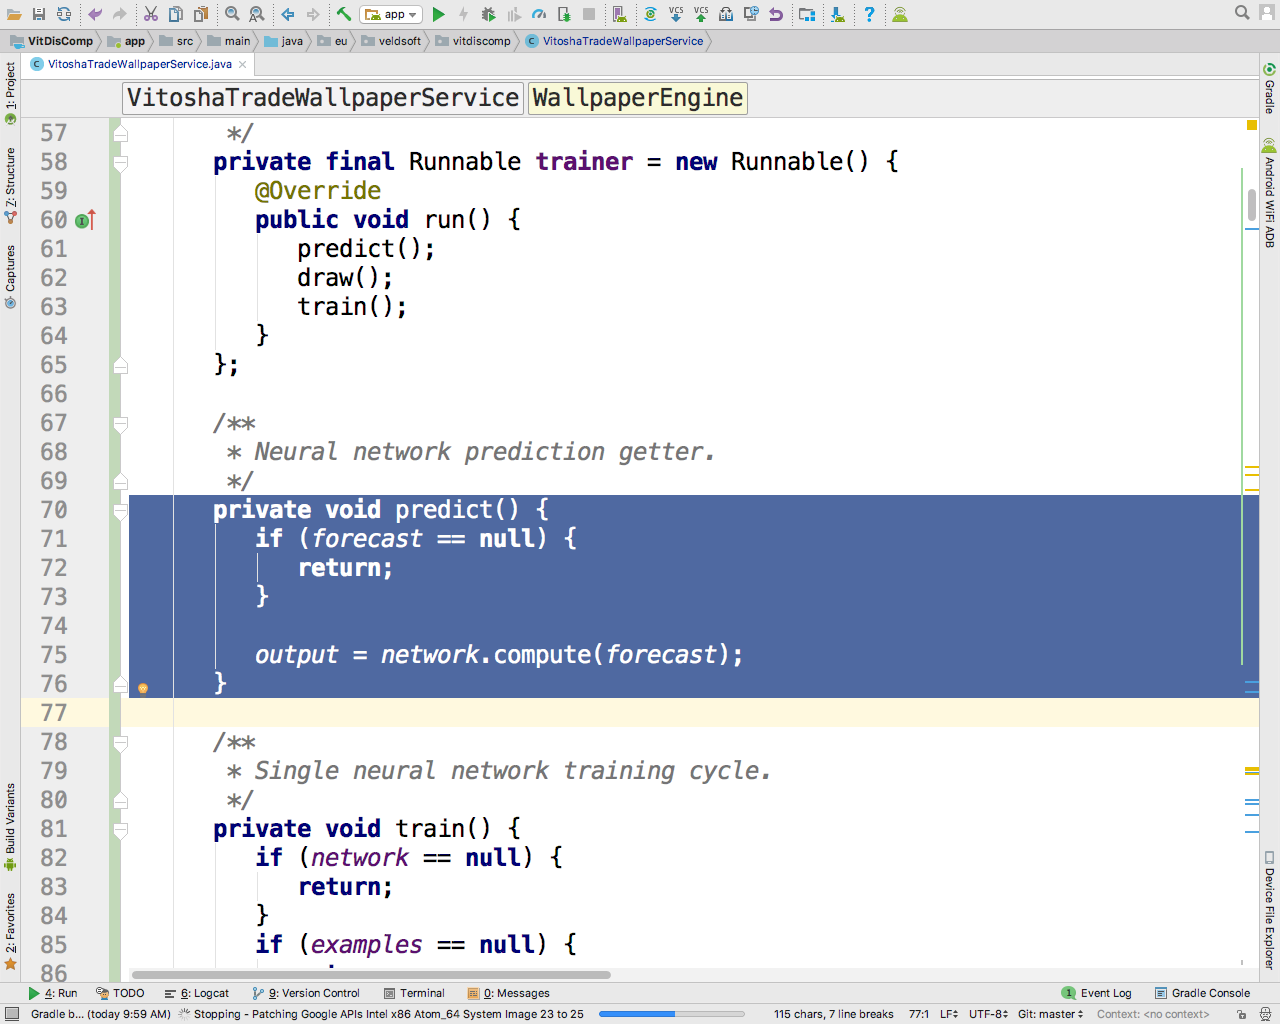
\includegraphics[height=0.45\pdfpageheight]{pic0048}
\caption{Prediction calculation}
\label{fig:pic0048}
\end{figure}
\FloatBarrier

To calculate a prediction, according to the current level of training of the artificial neural network\index{artificial neural networks}, it is enough to activate the network in working mode with appropriate data to the input layer (Fig. \ref{fig:pic0048}).

\begin{figure}[h]
\centering
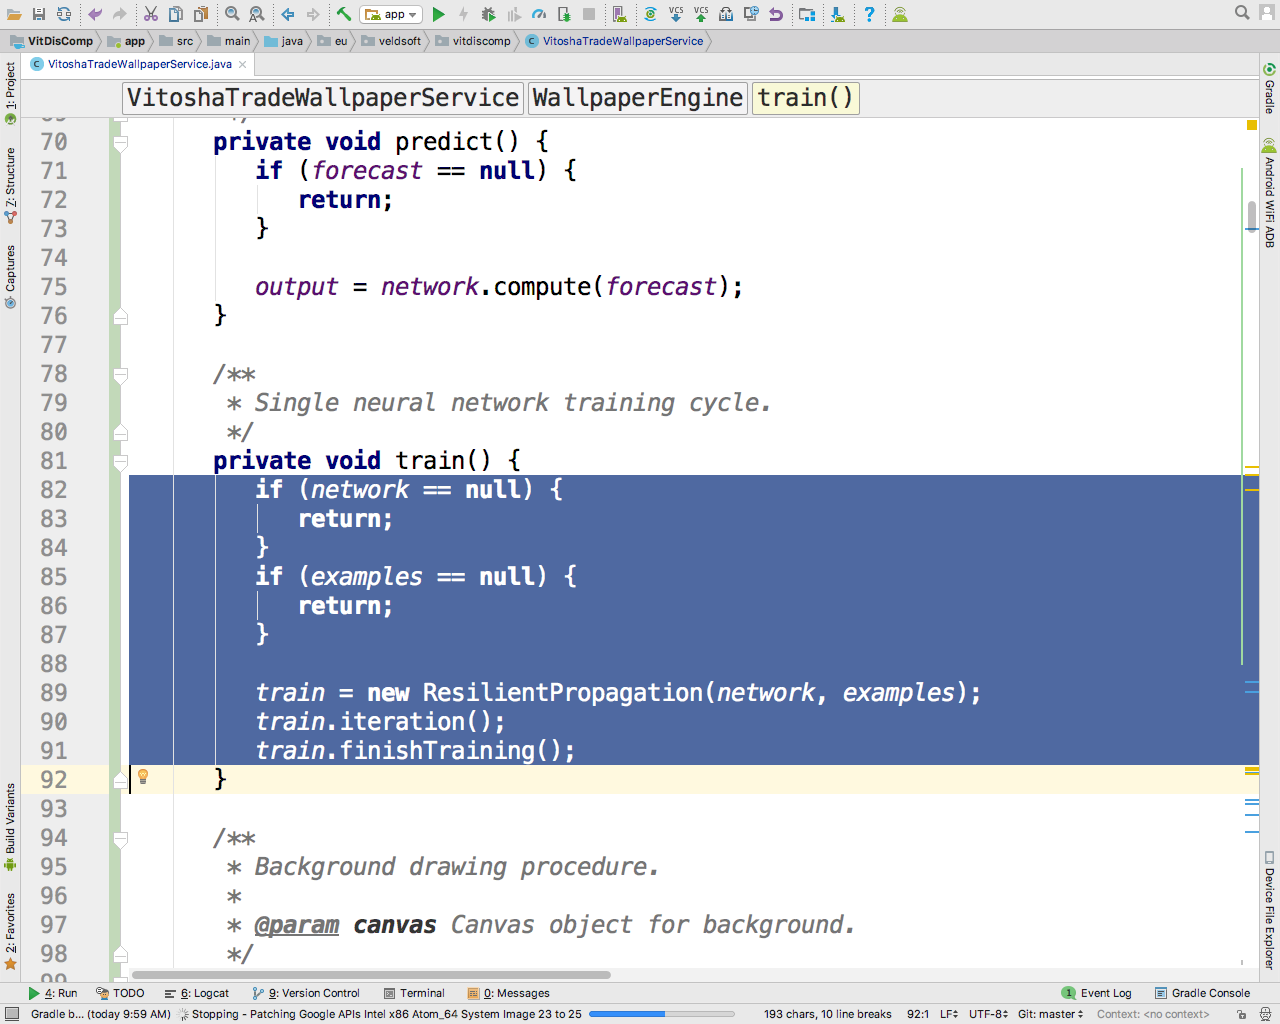
\includegraphics[height=0.45\pdfpageheight]{pic0049}
\caption{Training cycle of the artificial neural network}
\label{fig:pic0049}
\end{figure}
\FloatBarrier

To perform one training cycle of the artificial neural network\index{artificial neural networks}, it is enough to create a training object (in the case of elastic backpropagation of the error\index{backpropagation of the error}) to which the network and training examples are fed (Fig. \ref{fig:pic0049}).

\begin{figure}[h]
\centering
\includegraphics[height=0.45\pdfpageheight]{pic0050}
\caption{Basic procedure for plotting the information from the training process}
\label{fig:pic0050}
\end{figure}
\FloatBarrier

Drawing the information from the training process is organized in a separate function (Fig. \ref{fig:pic0050}). For the visual representation to take place, access is provided to the surface and the canvas it contains. At the very end of the visualization function, a decision is made whether to execute the next training cycle or abort execution.

\begin{figure}[h]
\centering
\includegraphics[height=0.45\pdfpageheight]{pic0051}
\caption{Breakdown of the visual representation task}
\label{fig:pic0051}
\end{figure}
\FloatBarrier

Good practices for writing programming code include breaking a single complex task into a group of multiple, more straightforward tasks. This principle has been applied to the visual representation by creating five auxiliary functions (Fig. \ref{fig:pic0051}). The first function draws a background, the second draw translucent areas for the panels, the third fills the panel with information about the currency pair, the fourth displays information in the panel about the current forecast, and the fifth a stylized model of the artificial neural network\index{artificial neural networks}.

\begin{figure}[h]
\centering
\includegraphics[height=0.45\pdfpageheight]{pic0052}
\caption{Paint the background}
\label{fig:pic0052}
\end{figure}
\FloatBarrier

A previously prepared image is loaded to draw the background, and a piece is cut from it to fit the screen's dimensions (Fig. \ref{fig:pic0052}). Which part of the image is used is determined randomly.

\begin{figure}[h]
\centering
\includegraphics[height=0.45\pdfpageheight]{pic0053}
\caption{Drawing service information areas}
\label{fig:pic0053}
\end{figure}
\FloatBarrier

Immediately after drawing the background, the semi-transparent spots are also drawn to represent the information from the learning process visually (Fig. \ref{fig:pic0053}). A translucency grip is needed to avoid the side effect of color blending between the service information and the background.

\begin{figure}[h]
\centering
\includegraphics[height=0.45\pdfpageheight]{pic0054}
\caption{Drawing currency pair information}
\label{fig:pic0054}
\end{figure}
\FloatBarrier

The information about the currency pair consists of the name and time interval of the financial time series (Fig. \ref{fig:pic0054}).

\begin{figure}[h]
\centering
\includegraphics[height=0.45\pdfpageheight]{pic0055}
\caption{Position and dimensions for the visual representation of the forecast}
\label{fig:pic0055}
\end{figure}
\FloatBarrier

The visual representation of the prediction requires slightly more complex calculations so that the input and output information fit within the specified blob. To accomplish this task, the coordinates and dimensions of the specified area are taken (Fig. \ref{fig:pic0055}).

\begin{figure}[h]
\centering
\includegraphics[height=0.45\pdfpageheight]{pic0056}
\caption{Width and height data range}
\label{fig:pic0056}
\end{figure}
\FloatBarrier

To visualize the data, it is essential to define the minimum and maximum values for the input-output as well as the number of values to be visualized (Fig. \ref{fig:pic0056}). In this case, the number of values for visual representation coincides with the sum of the number of input and the number of output signals.

\begin{figure}[h]
\centering
\includegraphics[height=0.45\pdfpageheight]{pic0057}
\caption{Cycles for visual presentation of the time series and forecast pillars}
\label{fig:pic0057}
\end{figure}
\FloatBarrier

The data for the elapsed period is shown in one color, and the forecast data in another color (Fig. \ref{fig:pic0057}). The visual presentation is a bar chart of the input data and the forecast.

\begin{figure}[h]
\centering
\includegraphics[height=0.45\pdfpageheight]{pic0058}
\caption{Topology of the artificial neural network being visualized}
\label{fig:pic0058}
\end{figure}
\FloatBarrier

In the third visual representation area, stylized information about the state of the artificial neural network is drawn\index{artificial neural networks}. The rectangular area is divided into five vertical zones: 1. Values of the neurons in the input layer; 2. Values of the weights between the input and the hidden layer; 3. Values of the neurons in the hidden layer; 4. Values of the weights between the hidden and output layers; 5. Values of neurons in the output layer (Fig. \ref{fig:pic0058}).

\begin{figure}[h]
\centering
\includegraphics[height=0.45\pdfpageheight]{pic0059}
\caption{Input and output scaling}
\label{fig:pic0059}
\end{figure}
\FloatBarrier

The input and output information is resized relative to the minimum and maximum values that the neurons in the output layer work with (Fig. \ref{fig:pic0059}). The formula for MinMax Scaling (\ref{equation04}) is attached.

\begin{equation}
\label{equation04}
X_{sc} = \frac{X-X_{min}}{X_{max}-X_{min}}
\end{equation}

In practice, neurons in the input layer should not have an activation function constraint since they only collect information from the outside world.

\begin{figure}[h]
\centering
\includegraphics[height=0.45\pdfpageheight]{pic0060}
\caption{Weight values between layers}
\label{fig:pic0060}
\end{figure}
\FloatBarrier

Next is determining the weights between the layers (Fig. \ref{fig:pic0060}).

\begin{figure}[h]
\centering
\includegraphics[height=0.45\pdfpageheight]{pic0061}
\caption{Scaling the values in the hidden layer}
\label{fig:pic0061}
\end{figure}
\FloatBarrier

And finally, for the middle vertical region, the values for the hidden layer are determined and scaled to the minimum, and maximum level of the activation function applied to it (Fig. \ref{fig:pic0061}).

\begin{figure}[h]
\centering
\includegraphics[height=0.45\pdfpageheight]{pic0062}
\caption{Normalize values for weights}
\label{fig:pic0062}
\end{figure}
\FloatBarrier

To visualize the information about the weights, it is necessary to normalize their values relative to the smallest and largest value among them (Fig. \ref{fig:pic0062}).

\begin{figure}[h]
\centering
\includegraphics[height=0.45\pdfpageheight]{pic0063}
\caption{Draw the topology}
\label{fig:pic0063}
\end{figure}
\FloatBarrier

Thus, the previously prepared data is easily visualized by a group of nested loops (Fig. \ref{fig:pic0063}).

\begin{figure}[h]
\centering
\includegraphics[height=0.45\pdfpageheight]{pic0064}
\caption{Engine constructor for the service}
\label{fig:pic0064}
\end{figure}
\FloatBarrier

The service engine constructor has the sole task of loading the execution thread (Fig \ref{fig:pic0064}).

\begin{figure}[h]
\centering
\includegraphics[height=0.45\pdfpageheight]{pic0065}
\caption{Change in active wallpaper visibility}
\label{fig:pic0065}
\end{figure}
\FloatBarrier

When the visibility of the active wallpaper is changed, an onVisibilityChanged event is fired, which determines whether the thread should be reactivated or its calling terminated (Fig. \ref{fig:pic0065}).

\begin{figure}[h]
\centering
\includegraphics[height=0.45\pdfpageheight]{pic0066}
\caption{Stop calculations when destroying draw surface}
\label{fig:pic0066}
\end{figure}
\FloatBarrier

In the event of destroying the drawing area, a flag to stop the calculations is raised, and the thread responsible for them is removed from the execution queue (Fig. \ref{fig:pic0066}).

\begin{figure}[h]
\centering
\includegraphics[height=0.45\pdfpageheight]{pic0067}
\caption{Size of drawing areas}
\label{fig:pic0067}
\end{figure}
\FloatBarrier

When a change occurs in the drawing area of the active wallpaper, a series of resizing measures must be taken. Such an event, for example, occurs when the device changes the visual representation from portrait to landscape or vice versa. The first feature to monitor is the size of the spots for a graphical representation (Fig. \ref{fig:pic0067}).


\begin{figure}[h]
\centering
\includegraphics[height=0.45\pdfpageheight]{pic0068}
\caption{Coordinates and dimensions of visual representation areas - top-left}
\label{fig:pic0068}
\end{figure}
\FloatBarrier

\begin{figure}[h]
\centering
\includegraphics[height=0.45\pdfpageheight]{pic0069}
\caption{Coordinates and dimensions of visual representation areas - top-center}
\label{fig:pic0069}
\end{figure}
\FloatBarrier

\begin{figure}[h]
\centering
\includegraphics[height=0.45\pdfpageheight]{pic0070}
\caption{Coordinates and dimensions of visual representation areas - top-right}
\label{fig:pic0070}
\end{figure}
\FloatBarrier

\begin{figure}[h]
\centering
\includegraphics[height=0.45\pdfpageheight]{pic0071}
\caption{Coordinates and dimensions of visual representation areas - center-left}
\label{fig:pic0071}
\end{figure}
\FloatBarrier

\begin{figure}[h]
\centering
\includegraphics[height=0.45\pdfpageheight]{pic0072}
\caption{Coordinates and dimensions of visual representation areas - center-center}
\label{fig:pic0072}
\end{figure}
\FloatBarrier

\begin{figure}[h]
\centering
\includegraphics[height=0.45\pdfpageheight]{pic0073}
\caption{Coordinates and dimensions of visual representation areas - center-right}
\label{fig:pic0073}
\end{figure}
\FloatBarrier

\begin{figure}[h]
\centering
\includegraphics[height=0.45\pdfpageheight]{pic0074}
\caption{Coordinates and dimensions of visual representation areas - bottom-left}
\label{fig:pic0074}
\end{figure}
\FloatBarrier

\begin{figure}[h]
\centering
\includegraphics[height=0.45\pdfpageheight]{pic0075}
\caption{Coordinates and dimensions of visual representation areas - bottom-center}
\label{fig:pic0075}
\end{figure}
\FloatBarrier

\begin{figure}[h]
\centering
\includegraphics[height=0.45\pdfpageheight]{pic0076}
\caption{Coordinates and dimensions of visual representation areas - bottom-right}
\label{fig:pic0076}
\end{figure}
\FloatBarrier

The user can choose the part of the active wallpaper where the visual presentation areas should be positioned. The horizontal options are left, center, and right, and the vertical options are top, center, and bottom.

\begin{figure}[h]
\centering
\includegraphics[height=0.45\pdfpageheight]{pic0077}
\caption{System load for background calculations}
\label{fig:pic0077}
\end{figure}
\FloatBarrier

The final feature that the user can control is to what extent their mobile device will be loaded with background calculations (Fig. \ref{fig:pic0077}).

\section{Presentation of the information on the local device}

The efficiency of calculations is significantly increased if the local computing nodes can store source data and calculated results locally.

\begin{figure}[h]
\centering
\includegraphics[height=0.45\pdfpageheight]{pic0078}
\caption{Time series interval constants (0 to 15)}
\label{fig:pic0078}
\end{figure}
\FloatBarrier

For the needs of this local representation, an auxiliary data type of enumerated type is used, which indicates the distance between two readings in the financial time series (Fig. \ref{fig:pic0078}, \ref{fig:pic0079}).

\begin{figure}[h]
\centering
\includegraphics[height=0.45\pdfpageheight]{pic0079}
\caption{Constants for time series intervals (30 to 43200)}
\label{fig:pic0079}
\end{figure}
\FloatBarrier

The intervals in the time series are determined based on the number of minutes, with the shortest interval being one minute. The intervals are described with two variables - name and number of minutes (Fig. \ref{fig:pic0080}).

\begin{figure}[h]
\centering
\includegraphics[height=0.45\pdfpageheight]{pic0080}
\caption{Time slot description}
\label{fig:pic0080}
\end{figure}
\FloatBarrier

The use of enumerated constants in Java makes it possible to elegantly use static functions to construct objects (Factory Method Design Pattern) that, after a given number (number of minutes), return the corresponding constant (Fig. \ref{fig:pic0081}).

\begin{figure}[h]
\centering
\includegraphics[height=0.45\pdfpageheight]{pic0081}
\caption{Defining an interval constant by number of minutes}
\label{fig:pic0081}
\end{figure}
\FloatBarrier

A similar effect can be achieved using the text description of the constants (Fig. \ref{fig:pic0082}).

\begin{figure}[h]
\centering
\includegraphics[height=0.45\pdfpageheight]{pic0082}
\caption{Defining an interval constant by textual description}
\label{fig:pic0082}
\end{figure}
\FloatBarrier

To prevent the creation of constants outside the enumerated type, it is assumed that the constructor has a private access level (Fig. \ref{fig:pic0083}).

\begin{figure}[h]
\centering
\includegraphics[height=0.45\pdfpageheight]{pic0083}
\caption{Constructor of the enumerated type for space}
\label{fig:pic0083}
\end{figure}
\FloatBarrier

The Android operating system provides reasonable means of storing information, including the SQLite relational database management system.

\begin{figure}[h]
\centering
\includegraphics[height=0.45\pdfpageheight]{pic0084}
\caption{Local table structure for quotations}
\label{fig:pic0084}
\end{figure}
\FloatBarrier

Information about the time series can be stored locally in a table with a suitable structure that reflects the presence of four values for each interval, the time of the interval, the traded volume, the name of the currency pair, and the size of the time interval (Fig. \ref{fig:pic0084}).

\begin{figure}[h]
\centering
\includegraphics[height=0.45\pdfpageheight]{pic0085}
\caption{Local Table Structure for Artificial Neural Networks}
\label{fig:pic0085}
\end{figure}
\FloatBarrier

An additional table takes care of the storage of the information about the artificial neural networks, which includes the name of the currency pair, the time interval, the value of the neurons, the value of the connections between the neurons, and the value of the weights between the neurons (Fig. \ref{fig:pic0085}).

\begin{figure}[h]
\centering
\includegraphics[height=0.45\pdfpageheight]{pic0086}
\caption{Database name and version}
\label{fig:pic0086}
\end{figure}
\FloatBarrier

Android manages databases in the form of a DB resource and an integer version for the structure (Fig. \ref{fig:pic0086}).

\begin{figure}[h]
\centering
\includegraphics[height=0.45\pdfpageheight]{pic0087}
\caption{Code to create the quote table}
\label{fig:pic0087}
\end{figure}
\FloatBarrier

\begin{figure}[h]
\centering
\includegraphics[height=0.45\pdfpageheight]{pic0088}
\caption{Code to create the artificial neural network table}
\label{fig:pic0088}
\end{figure}
\FloatBarrier

Parameterized symbolic constants control the creation of the tables (Fig. \ref{fig:pic0087}, \ref{fig:pic0088}).

\begin{figure}[h]
\centering
\includegraphics[height=0.45\pdfpageheight]{pic0089}
\caption{Code to delete the tables}
\label{fig:pic0089}
\end{figure}
\FloatBarrier

Deleting tables is also done with parameterized symbolic constants (Fig. \ref{fig:pic0089}).

\begin{figure}[h]
\centering
\includegraphics[height=0.45\pdfpageheight]{pic0090}
\caption{Constructor and virtual methods of the database helper class}
\label{fig:pic0090}
\end{figure}
\FloatBarrier

The constructor of the helper class for the database has the sole task of calling the parent class's constructor (Fig \ref{fig:pic0090}). The two predefined virtual functions call the requests to construct and update the database (Fig. \ref{fig:pic0090}).

\begin{figure}[h]
\centering
\includegraphics[height=0.45\pdfpageheight]{pic0091}
\caption{Type listed for neuron type}
\label{fig:pic0091}
\end{figure}
\FloatBarrier

The second type of data listed is regarding the type of neurons. In general, neurons can be regular, input, output, and bias (Fig. \ref{fig:pic0090}).

\begin{figure}[h]
\centering
\includegraphics[height=0.45\pdfpageheight]{pic0092}
\caption{An integer constant for the neuron type that can also be used as a bit field}
\label{fig:pic0092}
\end{figure}
\FloatBarrier

Since different connections between neurons are possible, neurons with more functions appear, such as: regular-input, regular-output, input-output, and input-regular-output. All possible combinations are recorded in an integer variable, which can also serve as a bit field (Fig. \ref{fig:pic0092}).

\begin{figure}[h]
\centering
\includegraphics[height=0.45\pdfpageheight]{pic0093}
\caption{Determining the enumerable constant by numeric value}
\label{fig:pic0093}
\end{figure}
\FloatBarrier

Since the information from the server arrives mainly in the form of numbers, it is rational to add a static function for constructing the object (Factory Method Design Pattern), which numerically determines the constant in the enumerated type (Fig. \ref{fig:pic0093}).

\begin{figure}[h]
\centering
\includegraphics[height=0.45\pdfpageheight]{pic0094}
\caption{Methods to access constant internal values}
\label{fig:pic0094}
\end{figure}
\FloatBarrier

For convenience, accessor methods are often used when working with constants and the information hidden in them. In this case, a public getter but a setter with private access. It makes sense to make the setter private to preserve the property of enumerated constants to stay constants (Fig \ref{fig:pic0094}).

\newpage
\chapter{Централизиран сървър}
\label{chapter05}

За да бъдат успешно извършени изчисленията в разпределена среда\index{изчисления в разпределена среда} освен наличието на множество устройства е от съществено значение да има централизирано място от което да бъдат раздавани задачите и където да бъдат събирани резултатите. Архитектура от тип клиент-сървър би била изключително удачна при едно техническо решение за не особено интензивна комуникация, която не изисква постоянна връзка между възлите. Приложението работещо на сървъра се състои от два компонента - база данни и работна логика. Изборът на системата за управление на бази от данни и скриптовия език на сървъра е обоснован основно с преследването на висока финансова ефективност. Към настоящия момент най-изгодно е използването на комбинацията MySQL и PHP, както е в проекта VitoshaTrade\cite{vtrade} (Фиг. \ref{fig:pic0095}).

\begin{figure}[h]
  \centering
  \includegraphics[height=0.45\pdfpageheight]{pic0095}
  \caption{Публично хранилище за кода на сървър приложението.}
\label{fig:pic0095}
\end{figure}
\FloatBarrier

\section{Релационна база данни}

За нуждите от съхраняването на информация от страна на сървъра е достатъчно да се разработи база от данни в която таблиците са нормализирани поне до трета нормална форма (Фиг. \ref{fig:pic0096}).

\begin{figure}[h]
  \centering
  \includegraphics[height=0.35\pdfpageheight]{pic0096}
  \caption{Физическа структура на базата данни.}
\label{fig:pic0096}
\end{figure}
\FloatBarrier

Това което всеки един финансов времеви ред има е интервал на който се извършват отчитанията на нивата. Тази информация се записва в таблица с три колони - служебен идентификатор, брой минути за интервала и символно название на интервала (Фиг. \ref{fig:pic0097}).

\begin{figure}[h]
  \centering
  \includegraphics[height=0.45\pdfpageheight]{pic0097}
  \caption{Таблица с времевите интервали за редовете.}
\label{fig:pic0097}
\end{figure}
\FloatBarrier

Най-съществената таблица в базата данни е таблицата за описване на валутните двойки (Фиг. \ref{fig:pic0098}). Тя съдържа следните полета - служебен идентификатор, название на валутната двойка, външен ключ към времевия интервал, отместване необходимо за нормализиране на информацията, множител за мащабиране, също необходим за нормализирането на информацията, описание на валутната двойка и маркер за време в което е направен записът в таблицата. 

\begin{figure}[h]
  \centering
  \includegraphics[height=0.45\pdfpageheight]{pic0098}
  \caption{Таблица за представяне на валутните двойки.}
\label{fig:pic0098}
\end{figure}
\FloatBarrier

Топологията на всяка невронна мрежа се описва само един път в таблица за видовете мрежи (Фиг. \ref{fig:pic0099}). Тази таблица съдържа следните полета - служебен идентификатор, външен ключ към валутната двойка за която се отнася мрежата, брой неврони, флагове за типа на невроните, стойности за връзките между невроните (според матрицата за съседство) и в кой момент от времето е направен записа в таблицата. 

\begin{figure}[h]
  \centering
  \includegraphics[height=0.45\pdfpageheight]{pic0099}
  \caption{Таблица за представяне на типовете мрежи.}
\label{fig:pic0099}
\end{figure}
\FloatBarrier

На всяка топология мрежа може да отговарят множество екземпляри от тип изкуствена невронна мрежа (Фиг. \ref{fig:pic0100}). Информацията която таблицата за екземплярите е организирана в следните колони - служебен идентификатор, външен ключ към типа мрежа за който се отнася екземплярът, жизнена стойност на екземпляра, тегла на връзките между невроните (по графа за съседство) и момент от времето в който е направен записът в таблицата. 

\begin{figure}[h]
  \centering
  \includegraphics[height=0.45\pdfpageheight]{pic0100}
  \caption{Таблица за представяне на типовете мрежи.}
\label{fig:pic0100}
\end{figure}
\FloatBarrier

За всеки екземпляр на невронна мрежа е важно да се знае при какви параметри протича обучението му (Фиг. \ref{fig:pic0101}). За тази цел е предназначена отделна таблица със следните колони - служебен идентификатор, външен ключ към екземпляра, размер на популацията (когато става въпрос за обучаващ генетичен алгоритъм), брой барове на входа и брой барове на изхода.

\begin{figure}[h]
  \centering
  \includegraphics[height=0.45\pdfpageheight]{pic0101}
  \caption{Таблица с опции за протичане на обучението.}
\label{fig:pic0101}
\end{figure}
\FloatBarrier

При нужда от визуализация на екземпляра за изкуствена невронна мрежа е удачно да се съхранява информация за координатите на всеки неврон в равнината xOy (Фиг. \ref{fig:pic0102}). Тази таблица съдържа следните колони - служебен идентификатор, външен ключ към екземпляра, координати на невроните по реда на тяхното срещане в екземпляра и маркер за времето в което е направен записът в таблицата. 

\begin{figure}[h]
  \centering
  \includegraphics[height=0.45\pdfpageheight]{pic0102}
  \caption{Таблица с опции за протичане на обучението.}
\label{fig:pic0102}
\end{figure}
\FloatBarrier

Последната, но изключително важна таблица, е таблицата за съхранение на обучаващите примери, съдържащи информацията за финансовия времеви ред (Фиг. \ref{fig:pic0103}). Тази таблица съдържа следните колони - служебен идентификатор, външен ключ към валутната двойка, брой измервания, последователност от времеви маркери, последователност от нива (отваряне, най-ниско, най-високо, затваряне), търгуван обем и времеви маркер за момента в който е направен записът в таблицата. 

\begin{figure}[h]
  \centering
  \includegraphics[height=0.45\pdfpageheight]{pic0103}
  \caption{Таблица с опции за протичане на обучението.}
\label{fig:pic0103}
\end{figure}
\FloatBarrier

\section{Алгоритмична обработка на суровите данни}

За да се постигне добро разделяне, според трислойната архитектура на системата, от съществено значение е суровите данни да бъдат минимално обвързани с работната логика. Често срещана практика е смесването на работата със суровите данни и програмния код от работната логика. Такова смесване лесно се получава, ако в скриптовете от работната логика се изпълняват сложни SQL заявки. Подобен начин за конструиране на сървърното приложение прави системата трудна за поддържане и още по-трудна за реорганизиране, ако се наложи смяна на системата за управление на бази от данни или инструментите използвани в слоя на работната логика. Добро разделяне между двата слоя се получава когато работната логика, под формата на SQL заявки, единствено вика съхранени функции и процедури (stored procedures) на системата за управление на бази от данни. От една страна синтаксисът на заявките в междинния слой става максимално опростен, от друга страна евентуална подмяна на базата данни би довела до единствена корекция в начина по който се извикват съхранените функции и процедури. За да се удовлетвори стремежа за максимално разделяне между слоевете, към структурата на базата данни са добавени група съхранени функции и процедури. 

\begin{figure}[h]
  \centering
  \includegraphics[height=0.45\pdfpageheight]{pic0104}
  \caption{Процедура за добавяне на валутна двойка.}
\label{fig:pic0104}
\end{figure}
\FloatBarrier

При добавянето на нова валутна двойка, като входни данни постъпва названието на валутната двойка и времевия интервал (в брой минути), който интервал трябва да бъде съпоставен на интервалите изброени в таблицата с времеви интервали. Това налага използването на съхранена процедура, която да извърши обработката на входната информация (Фиг. \ref{fig:pic0104}). 

\begin{figure}[h]
  \centering
  \includegraphics[height=0.45\pdfpageheight]{pic0105}
  \caption{Процедура за запис на екземпляр от изкуствена невронна мрежа.}
\label{fig:pic0105}
\end{figure}
\FloatBarrier

При записването на екземпляр от изкуствена невронна мрежа към базата данни постъпва информация за валутната двойка, периода на времевия ред, броя и типовете на невроните, матрици на съседство за връзките и жизнена оценка на екземпляра (Фиг. \ref{fig:pic0105}). Преди екземплярът да бъде добавен в таблицата с екземплярите се проверява дали валутната дойка е налична и се определя нейния идентификатор. Ако валутната двойка не е налична, то тя се създава. Следва проверка за съществуването на типа мрежа. Ако не съществува, то тя се създава. Последната инструкция е самото добавяне на екземпляра към таблицата с екземплярите. При така подбраната стратегия за работа максимално се спазват правилата за съблюдаване на референциалния интегритет. 

\begin{figure}[h]
  \centering
  \includegraphics[height=0.45\pdfpageheight]{pic0106}
  \caption{Процедура за запис на тренировъчни примери.}
\label{fig:pic0106}
\end{figure}
\FloatBarrier

При записа на тренировъчни примери, на входа на базата данни се подават серия параметри за стойностите на времевия ред (Фиг. \ref{fig:pic0106}). По аналогичен начин се извършва проверка за съществуване на валутната двойка. Следва изтриване на предишни тренировъчни примери, ако такива бъдат открити. Финалната стъпка е добавянето на постъпилата информация. 

\begin{figure}[h]
  \centering
  \includegraphics[height=0.45\pdfpageheight]{pic0107}
  \caption{Функция за определяне на типа мрежа.}
\label{fig:pic0107}
\end{figure}
\FloatBarrier

Помощна функция определя служебния идентификатор на типа мрежа по описанието на екземпляр (Фиг. \ref{fig:pic0107}). Ако не бъде открит такъв тип служебно се връща нулева стойност. 

\begin{figure}[h]
  \centering
  \includegraphics[height=0.45\pdfpageheight]{pic0108}
  \caption{Функция за определяне на типа валутна двойка.}
\label{fig:pic0108}
\end{figure}
\FloatBarrier

По аналогичен начин, помощна функция служи за определяне на служебния идентификатор за валутна двойка, чрез зададено символно име и период (Фиг. \ref{fig:pic0108}). Ако валутната двойка не бъде открита се връща служебна нула. 

\begin{figure}[h]
  \centering
  \includegraphics[height=0.45\pdfpageheight]{pic0109}
  \caption{Функция за определяне на най-добрата жизненост.}
\label{fig:pic0109}
\end{figure}
\FloatBarrier

По зададено описание на изкуствена невронна мрежа, клиентските мобилни устройства запитват сървъра, на определени интервали от време, колко е стойността на най-жизнената мрежа. Това запитване е съществено, тъй като по него се взема решение дали мобилното устройство да докладва резултатите си на сървъра. Обработката се извършва на две стъпки - първо се намират всички мрежи с идентична топология, а след това се определя най-добрата жизненост (Фиг. \ref{fig:pic0109}).

\begin{figure}[h]
  \centering
  \includegraphics[height=0.45\pdfpageheight]{pic0110}
  \caption{Функция за определяне на броя неврони за определен еземпляр мрежа.}
\label{fig:pic0110}
\end{figure}
\FloatBarrier

Помощна функция определя и броя неврони по зададен идентификатор на екземпляр мрежа (Фиг. \ref{fig:pic0110}).

\section{Сървър скриптове}

Директният достъп до базата данни (TCP свързване) често е нежелателен, тъй като създава определени опасности за сигурността на данните. Поради тази причина е прието да се използва междинен слой, който да осъществява комуникацията с базата данни. За нуждите на настоящата разработка това са група PHP скриптове. 

\begin{figure}[h]
  \centering
  \includegraphics[height=0.45\pdfpageheight]{pic0111}
  \caption{Глобални променливи за достъп до базата данни.}
\label{fig:pic0111}
\end{figure}
\FloatBarrier

В специално отделен за целта файл (db.php) се задават следните глобални променливи за достъп до базата данни - хост на който е разположен MySQL сървърът, потребител в MySQL, парола на потребителя, название на базата данни и връзка (Фиг. \ref{fig:pic0111}).

\begin{figure}[h]
  \centering
  \includegraphics[height=0.45\pdfpageheight]{pic0112}
  \caption{Отваряне на връзка към базата данни.}
\label{fig:pic0112}
\end{figure}
\FloatBarrier

Две помощни функции служат за отваряне и затваряне на връзка към базата данни (Фиг. \ref{fig:pic0112}, \ref{fig:pic0113}).

\begin{figure}[h]
  \centering
  \includegraphics[height=0.45\pdfpageheight]{pic0113}
  \caption{Затваряне на връзката към базата данни.}
\label{fig:pic0113}
\end{figure}
\FloatBarrier

Допълнителна помощна функция изпълнява заявките към базата данни и връща резултата от изпълнението под формата на двумерен масив (Фиг. \ref{fig:pic0114}).

\begin{figure}[h]
  \centering
  \includegraphics[height=0.45\pdfpageheight]{pic0114}
  \caption{Изпълнение на заявки към базата данни.}
\label{fig:pic0114}
\end{figure}
\FloatBarrier

На този етап в разработката клиентското приложение изпраща своите данни под формата на POST заявка, а сървърът отговаря с JSON съобщение. Макар и спестяващ допълнителна работа около съставянето на JSON съобщения от страна на клиента, този подход не е за препоръчване и е желателно клиентите също да изпращат информацията в JSON формат, така че да се спазват конвенциите на RESTful приложенията. 

\subsection{Зареждане на мрежа по идентификатор}

Всеки екземпляр на изкуствена неверонна мрежа има служебен идентификатори, който представлява и първичен ключ в съответната таблица. За да бъде заредена мрежата се извиква PHP скрипт изпълняващ тази задача. 

\begin{figure}[h]
  \centering
  \includegraphics[height=0.45\pdfpageheight]{pic0115}
  \caption{Проверка на входните данни.}
\label{fig:pic0115}
\end{figure}
\FloatBarrier

Преди същинското зареждане на мрежата се включва модула за работа с базата данни и се извършва проверка на входните параметри. В случая единственият параметър е цяло число което е идентификатор на екземпляра (Фиг. \ref{fig:pic0115}).

\begin{figure}[h]
  \centering
  \includegraphics[height=0.45\pdfpageheight]{pic0116}
  \caption{Заявка за извличане на екземпляр по идентификатор.}
\label{fig:pic0116}
\end{figure}
\FloatBarrier

Следва отваряне на връзка към базата данни, съставяне на заявка (добрата практика изисква извикване на съхранена функция) и изпълнение на заявката (Фиг. \ref{fig:pic0116}). 

\begin{figure}[h]
  \centering
  \includegraphics[height=0.45\pdfpageheight]{pic0117}
  \caption{Проверка за наличност на екземпляра.}
\label{fig:pic0117}
\end{figure}
\FloatBarrier

Възможни са два изхода от изпълнението на заявката, спрямо това дали такъв екземпляр присъства в базата данни или не присъства. Ако екземплярът бъде открит започва изграждането на JSON съобщение с отговор към клиента. Отговорът съдържа единица, за намерен екземпляр, названието на валутната двойка, интервала на времевия ред, жизнената стойност на екземпляра, брой и типове на невроните, матрица на връзките и матрица на теглата (Фиг. \ref{fig:pic0117}-\ref{fig:pic0120}).

\begin{figure}[h]
  \centering
  \includegraphics[height=0.45\pdfpageheight]{pic0118}
  \caption{Информация за невроните.}
\label{fig:pic0118}
\end{figure}
\FloatBarrier

\begin{figure}[h]
  \centering
  \includegraphics[height=0.45\pdfpageheight]{pic0119}
  \caption{Информация за връзките.}
\label{fig:pic0119}
\end{figure}
\FloatBarrier

\begin{figure}[h]
  \centering
  \includegraphics[height=0.45\pdfpageheight]{pic0120}
  \caption{Информация за теглата.}
\label{fig:pic0120}
\end{figure}
\FloatBarrier

В ситуацията когато екземплярът не е открит се връща нулев флаг. И при двата случая (открит или не) JSON съобщението се завършва, базата данни се затваря и информацията се изпраща към клиента (Фиг. \ref{fig:pic0121}).

\begin{figure}[h]
  \centering
  \includegraphics[height=0.45\pdfpageheight]{pic0121}
  \caption{Приключване на процедурата по изпращане на отговор.}
\label{fig:pic0121}
\end{figure}
\FloatBarrier

\subsection{Зареждане на случайно избрана мрежа}

Когато изчисленията се извършват на принципа за дарената изчислителна мощност, коя мрежа ще бъде допълнително тренирана е логично да се избира на случаен принцип. За тази цел, скриптът от страна на сървъра избира мрежата по случаен начин.

\begin{figure}[h]
  \centering
  \includegraphics[height=0.45\pdfpageheight]{pic0157}
  \caption{Заявка за зареждане на случайна мрежа.}
\label{fig:pic0157}
\end{figure}
\FloatBarrier

Единствената разлика от зареждането на мрежа по идентификатори и случайно избрана мрежа е в SQL заявката, която се изпълнява от MySQL (Фиг. \ref{fig:pic0157}).

\subsection{Зареждане на най-добрата жизненост от глобалната популация}

Един от основните критерии по които клиентските приложения вземат решение дали да докладват откритите от тях резултати е стойността на най-добрата жизненост в глобалната популация (популацията, която се съхранява на сървъра). Скриптът отговарящ за тази проверка също включва модула за работа с базата данни и извършва серия проверки на входните параметри. 

\begin{figure}[h]
  \centering
  \includegraphics[height=0.45\pdfpageheight]{pic0122}
  \caption{Входни параметри за конкретна топология на невронна мрежа.}
\label{fig:pic0122}
\end{figure}
\FloatBarrier

Проверяват се названието на валутната двойка, периода на времевия ред, броят и типовете на невроните, както и връзките между тях (Фиг. \ref{fig:pic0122}).

\begin{figure}[h]
  \centering
  \includegraphics[height=0.45\pdfpageheight]{pic0123}
  \caption{Флагове на невроните и връзките между тях.}
\label{fig:pic0123}
\end{figure}
\FloatBarrier

Тъй като типовете на невроните са представени като масив, а връзките между самите неврони в матрица на съседство, то проверката им изисква малко по-сложна обработка в цикли (Фиг. \ref{fig:pic0123}).

\begin{figure}[h]
  \centering
  \includegraphics[height=0.45\pdfpageheight]{pic0124}
  \caption{Заявка за най-добра жизненост.}
\label{fig:pic0124}
\end{figure}
\FloatBarrier

Следва отваряне на връзката към базата данни, изпълнение на съхранената функция за откриване на най-добра жизненост, затваряне на базата данни и изпращане до клиента на JSON пакетиран отговор (Фиг. \ref{fig:pic0124}).

\subsection{Зареждане на брой неврони по идентификатор}

При работата с екземпляри на изкуствените невронни мрежи съществено е запитването за броя неврони в мрежата. 

\begin{figure}[h]
  \centering
  \includegraphics[height=0.45\pdfpageheight]{pic0125}
  \caption{Определяне на броя неврони по идентификатор на мрежа.}
\label{fig:pic0125}
\end{figure}
\FloatBarrier

Процедурата отново включва модула за работа с базата данни, проверка на входния параметър за идентификатор на екземпляр, отваряне на връзка към базата данни и стартиране на съхранен функция (Фиг. \ref{fig:pic0125}).

\begin{figure}[h]
  \centering
  \includegraphics[height=0.45\pdfpageheight]{pic0126}
  \caption{Отговор към клиента.}
\label{fig:pic0126}
\end{figure}
\FloatBarrier

Резултатът от съхранената функция се опакова в JSON съобщение и се изпраща на клиента (Фиг. \ref{fig:pic0126}).

\subsection{Зареждане на тренировъчно множество по информация за валутна двойка}

За обучението на всяка изкуствена неверонна мрежа се използва тренировъчно множество, което е различно, според названието на валутната двойка и времевия интервал на реда. 

\begin{figure}[h]
  \centering
  \includegraphics[height=0.45\pdfpageheight]{pic0127}
  \caption{Проверка на входните параметри.}
\label{fig:pic0127}
\end{figure}
\FloatBarrier

Зареждането започва по класическия начин с включване на модула за работа с базата данни, проверка на входната информация и отваряне на връзка към базата данни (Фиг. \ref{fig:pic0127}).

\begin{figure}[h]
  \centering
  \includegraphics[height=0.45\pdfpageheight]{pic0128}
  \caption{Заявка за тренировъчно множество.}
\label{fig:pic0128}
\end{figure}
\FloatBarrier

Следва заявка, извличане на резултата и затваряне на връзката към базата данни (Фиг. \ref{fig:pic0128}). Макар и да не е направено, добрият стил за разделяне на слоевете предполага вместо заявка да се извика съхранена функция. 

\begin{figure}[h]
  \centering
  \includegraphics[height=0.45\pdfpageheight]{pic0129}
  \caption{Брой примери, времеви маркери и нива на отваряне.}
\label{fig:pic0129}
\end{figure}
\FloatBarrier

\begin{figure}[h]
  \centering
  \includegraphics[height=0.45\pdfpageheight]{pic0130}
  \caption{Най-ниска и най-висока постигната стойност.}
\label{fig:pic0130}
\end{figure}
\FloatBarrier

\begin{figure}[h]
  \centering
  \includegraphics[height=0.45\pdfpageheight]{pic0131}
  \caption{Нива на затваряне и търгуван обем.}
\label{fig:pic0131}
\end{figure}
\FloatBarrier

Ако е намерено тренировъчно множество за посочената валутна двойка и времеви интервал, то стойностите от времевия ред се пакетират и изпращат на клиента (Фиг. \ref{fig:pic0129}-\ref{fig:pic0131}).

\begin{figure}[h]
  \centering
  \includegraphics[height=0.45\pdfpageheight]{pic0132}
  \caption{Изпращане на отговор до клиента.}
\label{fig:pic0132}
\end{figure}
\FloatBarrier

Ако тренировъчно множество не бъде открито се изпраща съобщение с нулев размер за данните. Без значение дали е открито множество или не, JSON съобщението се изпраща до клиента (Фиг. \ref{fig:pic0132}).

\subsection{Зареждане на брой екземпляри по идентификатор или информация за валутна двойка}

За подбирането на подмножество от глобалната популация е нужно да се знае колко екземпляра присъстват в базата данни по зададен идентификатор на екземпляр или название на валутна двойка с период. 

\begin{figure}[h]
  \centering
  \includegraphics[height=0.45\pdfpageheight]{pic0133}
  \caption{Проверка на входните аргументи.}
\label{fig:pic0133}
\end{figure}
\FloatBarrier

Проверката отново започва с включване на модула за работа с базата данни, проверка на входните аргументи и отваряне на връзка към базата данни (Фиг. \ref{fig:pic0133}).

\begin{figure}[h]
  \centering
  \includegraphics[height=0.45\pdfpageheight]{pic0134}
  \caption{Еземпляри от типа на подадения идентификатор.}
\label{fig:pic0134}
\end{figure}
\FloatBarrier

Първо се изброяват екземплярите които са от типа на подадения идентификатор (Фиг. \ref{fig:pic0134}).

\begin{figure}[h]
  \centering
  \includegraphics[height=0.45\pdfpageheight]{pic0135}
  \caption{Пакетиране на получените стойности в JSON съобщение.}
\label{fig:pic0135}
\end{figure}
\FloatBarrier

Получените стойности се пакетират в JSON съобщение (Фиг. \ref{fig:pic0135}). 

\begin{figure}[h]
  \centering
  \includegraphics[height=0.45\pdfpageheight]{pic0136}
  \caption{Проверка за екземпляри по название на валутна двойка и период.}
\label{fig:pic0136}
\end{figure}
\FloatBarrier

Следва проверка за екземпляри по название на валутна двойка и период. Този списък се използва само, ако първоначално не е открито подмножество (Фиг. \ref{fig:pic0136}).

\begin{figure}[h]
  \centering
  \includegraphics[height=0.45\pdfpageheight]{pic0137}
  \caption{Пакетиране на получените стойности в JSON съобщение.}
\label{fig:pic0137}
\end{figure}
\FloatBarrier

Пакетирането в JSON съобщение е аналогично на предходното (Фиг. \ref{fig:pic0137}).

\begin{figure}[h]
  \centering
  \includegraphics[height=0.45\pdfpageheight]{pic0138}
  \caption{Изпращане на резултата.}
\label{fig:pic0138}
\end{figure}
\FloatBarrier

Скриптът завършва със затваряне на връзката към базата данни, оформяне и изпращане на резултата до клиента (Фиг. \ref{fig:pic0138}).

\subsection{Зареждане на брой тренировъчни примери по информация за валутна двойка}

За определянето на броя тренировъчни примери се подхожда по аналогичен начин с включване на модула за работа с базата данни, проверка на входните аргументи и отваряне на връзка към базата данни (Фиг. \ref{fig:pic0139}). 

\begin{figure}[h]
  \centering
  \includegraphics[height=0.45\pdfpageheight]{pic0139}
  \caption{Брой тренировъчни примери по валутна информация.}
\label{fig:pic0139}
\end{figure}
\FloatBarrier

Изпълнението на заявката може да открие подходящо тренировъчно множество или да не открие такова (Фиг. \ref{fig:pic0140}). 

\begin{figure}[h]
  \centering
  \includegraphics[height=0.45\pdfpageheight]{pic0140}
  \caption{Заявка за брой тренировъчни примери.}
\label{fig:pic0140}
\end{figure}
\FloatBarrier

Скриптът приключва със затваряне на връзката към базата данни, пакетиране и изпращане на отговора до клиента (Фиг. \ref{fig:pic0141}).

\begin{figure}[h]
  \centering
  \includegraphics[height=0.45\pdfpageheight]{pic0141}
  \caption{Изпращане на отговор до клиента.}
\label{fig:pic0141}
\end{figure}
\FloatBarrier

\subsection{Съхнраняване на екземпляр изкуствена невронна мрежа}

Съхраняването на екземпляр от изкуствената невронна мрежа не връща резултат за изпълнението на операцията и поради тази причина не се използва JSON. След включването на модула за работа с базата от данни се изисква по-сложна проверка на входните аргументи, тъй като те са повече на брой и по-сложни (Фиг. \ref{fig:pic0142}-\ref{fig:pic0146}). 

\begin{figure}[h]
  \centering
  \includegraphics[height=0.45\pdfpageheight]{pic0142}
  \caption{Проверка на входните аргументи за валутна двойка, период, жизненост и брой неврони.}
\label{fig:pic0142}
\end{figure}
\FloatBarrier

\begin{figure}[h]
  \centering
  \includegraphics[height=0.45\pdfpageheight]{pic0143}
  \caption{Проверка на входните аргументи за флагове на невроните, връзки и тегла между невроните.}
\label{fig:pic0143}
\end{figure}
\FloatBarrier

\begin{figure}[h]
  \centering
  \includegraphics[height=0.45\pdfpageheight]{pic0144}
  \caption{Проверка за типа на всеки неврон.}
\label{fig:pic0144}
\end{figure}
\FloatBarrier

\begin{figure}[h]
  \centering
  \includegraphics[height=0.45\pdfpageheight]{pic0145}
  \caption{Проверка за стойността на всяко тегло.}
\label{fig:pic0145}
\end{figure}
\FloatBarrier

\begin{figure}[h]
  \centering
  \includegraphics[height=0.45\pdfpageheight]{pic0146}
  \caption{Проверка за стойността на всяка връзка.}
\label{fig:pic0146}
\end{figure}
\FloatBarrier

При този скрипт проверките са значително по-сложни, тъй като освен наличност на аргументите се следи за числените стойности, които пристигат от клиентското приложение. 

\begin{figure}[h]
  \centering
  \includegraphics[height=0.45\pdfpageheight]{pic0147}
  \caption{Съхнраняване на екземпляр изкуствена невронна мрежа.}
\label{fig:pic0147}
\end{figure}
\FloatBarrier

Същината на скрипта представлява отваряне на връзка към базата данни, изпълнение на съхранена процедура и затваряне на връзката към базата данни (Фиг. \ref{fig:pic0147}).

\subsection{Съхнраняване на екземпляр изкуствена невронна мрежа след дообучение}

Когато определена изкуствена невронна мрежа е преминала допълнителен цикъл на обучение и бъде изпратена до отдалечения сървър, разумно е информацията да се съхранява само ако води до подобряване на жизнеността. 

\begin{figure}[h]
  \centering
  \includegraphics[height=0.45\pdfpageheight]{pic0158}
  \caption{Проверка на жизнеността преди съхраняване на информацията.}
\label{fig:pic0158}
\end{figure}
\FloatBarrier

Разликата между общата процедура за съхраняване на изкуствена невронна мрежа и съхраняването след допълнително обучение е в проверката на най-добрата постигната жизнена стойност (Фиг. \ref{fig:pic0158}).

\subsection{Съхнраняване на тренировъчно множество}

По аналогичен начин, при съхраняването на тренировъчни примери не се връща JSON съобщение и кода по проверката на входните данни превъзхожда кода за самото съхраняване. Първоначално се проверява наличието на аргументите (Фиг. \ref{fig:pic0148},\ref{fig:pic0149}).

\begin{figure}[h]
  \centering
  \includegraphics[height=0.45\pdfpageheight]{pic0148}
  \caption{Проверка на агументите за валутна двойка, период, брой примери и времеви маркери.}
\label{fig:pic0148}
\end{figure}
\FloatBarrier

\begin{figure}[h]
  \centering
  \includegraphics[height=0.45\pdfpageheight]{pic0149}
  \caption{Проверка на агументите за отваряне, най-ниска стойност, най-висока стойност, затваряне и изтъргуван обем.}
\label{fig:pic0149}
\end{figure}
\FloatBarrier

Всеки от масивите преминава допълнителна проверка за стойностите които съдържа (Фиг. \ref{fig:pic0150}-\ref{fig:pic0152}).

\begin{figure}[h]
  \centering
  \includegraphics[height=0.45\pdfpageheight]{pic0150}
  \caption{Проверка на стойностите за времеви маркери и нива на отваряне.}
\label{fig:pic0150}
\end{figure}
\FloatBarrier

\begin{figure}[h]
  \centering
  \includegraphics[height=0.45\pdfpageheight]{pic0151}
  \caption{Проверка на стойностите за най-ниско и най-високо постигнато ниво.}
\label{fig:pic0151}
\end{figure}
\FloatBarrier

\begin{figure}[h]
  \centering
  \includegraphics[height=0.45\pdfpageheight]{pic0152}
  \caption{Проверка на стойностите за затваряне и изтъргуван обем.}
\label{fig:pic0152}
\end{figure}
\FloatBarrier

Същинската част на скрипта отваря връзка към базата данни, изпълнява съхранена процедура и затваря връзката към базата данни (Фиг. \ref{fig:pic0153}).

\begin{figure}[h]
  \centering
  \includegraphics[height=0.45\pdfpageheight]{pic0153}
  \caption{Съхраняване на тренировъчно множество.}
\label{fig:pic0153}
\end{figure}
\FloatBarrier
\newpage
\chapter{Client-Server Communication}
\label{chapter06}

Communication between the Android client and the PHP based server is done over HTTP with the exchange of JSON packed messages.

\section{Hypertext Transfer Protocol}

Each time a wallpaper instance is created, a connection to the remote server must be made and a job package requested. If the connection is not possible, the data stored in the local database is used.

\begin{figure}[h]
\centering
\includegraphics[height=0.45\pdfpageheight]{pic0155}
\caption{Initialization of internal variables}
\label{fig:pic0155}
\end{figure}
\FloatBarrier

Internal variables are initialized in the onCreate event (Fig. \ref{fig:pic0155}).

\begin{figure}[h]
\centering
\includegraphics[height=0.45\pdfpageheight]{pic0156}
\caption{Loading data using HTTP communication}
\label{fig:pic0156}
\end{figure}
\FloatBarrier

The initialization of internal variables over HTTP is taken over by an additional created helper object, which is of a class responsible for communication (Fig. \ref{fig:pic0156}).

\begin{figure}[h]
\centering
\includegraphics[height=0.45\pdfpageheight]{pic0159}
\caption{HTTP communication file}
\label{fig:pic0159}
\end{figure}
\FloatBarrier

The HTTP communication with the remote server and the parsing of the JSON messages are exported to the HttpHelper helper class (Fig. \ref{fig:pic0159}). There are various ways to set the names used for remote scripts, but one of the most basic is through named constants. Server script names are subject to change, but this is expected to be significantly less frequent than changing the URL. It is precisely for this reason that the information is parameterized in a different way.

\begin{figure}[h]
\centering
\includegraphics[height=0.45\pdfpageheight]{pic0162}
\caption{Helper class constructor}
\label{fig:pic0162}
\end{figure}
\FloatBarrier

Since the URL of the remote server is likely to change multiple times, it is wise to pass this information into the class constructor (Fig. \ref{fig:pic0162}).

\begin{figure}[h]
\centering
\includegraphics[height=0.45\pdfpageheight]{pic0163}
\caption{Function to load a random network selected by the server}
\label{fig:pic0163}
\end{figure}
\FloatBarrier

To spawn a random network, the designated script on the remote server is called. This is done in an auxiliary function load, which loads the information into the publicly available global structure for representing the working data (Fig. \ref{fig:pic0163}).

\begin{figure}[h]
\centering
\includegraphics[height=0.45\pdfpageheight]{pic0167}
\caption{Loading training set}
\label{fig:pic0167}
\end{figure}
\FloatBarrier

After a randomly selected network is loaded, a training set suitable for the network is also loaded (Fig. \ref{fig:pic0167}). To compare the available time series, the name of the symbol pair and the period of the series are used.

\begin{figure}[h]
\centering
\includegraphics[height=0.45\pdfpageheight]{pic0164}
\caption{Function to save additional trained network}
\label{fig:pic0164}
\end{figure}
\FloatBarrier

In the process of storing the additionally trained network, a second helper function save is used, which aims to send, by HTTP request, the information available in the global structure with the training data (Fig. \ref{fig:pic0164}).

\begin{figure}[h]
\centering
\includegraphics[height=0.45\pdfpageheight]{pic0165}
\caption{Preparing a POST request}
\label{fig:pic0165}
\end{figure}
\FloatBarrier

The data from the global structure is formed as an HTTP request of the POST type, which is related to its transformation from binary values to text (Fig. \ref{fig:pic0165}).

\begin{figure}[h]
\centering
\includegraphics[height=0.45\pdfpageheight]{pic0166}
\caption{Executing the POST request}
\label{fig:pic0166}
\end{figure}
\FloatBarrier

Sending the information ends with the execution of the HTTP request (Fig. \ref{fig:pic0166}).

\section{JavaScript Object Notation}

Once received over HTTP, the JSON-packaged information is parsed and transformed from a stream of bytes into the internal structure to represent a packet for computation.

\begin{figure}[h]
\centering
\includegraphics[height=0.45\pdfpageheight]{pic0160}
\caption{Key values to describe the network}
\label{fig:pic0160}
\end{figure}
\FloatBarrier

One of the main roles of JSON is in the construction of communication protocols, which in the present development consists of information organized hierarchically on the "key-value" principle. Since communication protocols are subject to change, it is convenient to represent key values in the form of renamed constants (Fig. \ref{fig:pic0160},\ref{fig:pic0161}).

\begin{figure}[h]
\centering
\includegraphics[height=0.45\pdfpageheight]{pic0161}
\caption{Key values to describe the training set}
\label{fig:pic0161}
\end{figure}
\FloatBarrier

When loading an artificial neural network and its training timeline from the remote server, the information is obtained with two separate HTTP requests. This requires two separate fragments to process the JSON messages.

\begin{figure}[h]
\centering
\includegraphics[height=0.45\pdfpageheight]{pic0168}
\caption{Values for time series and neurons}
\label{fig:pic0168}
\end{figure}
\FloatBarrier

The first fragment provides information about the type of time series, the period of the time series, the number of neurons in the network and their type (Fig. \ref{fig:pic0168}), values of weights and values for the strength of connections between neurons (Fig. \ref{fig:pic0169}).

\begin{figure}[h]
\centering
\includegraphics[height=0.45\pdfpageheight]{pic0169}
\caption{Values for link weights and strengths}
\label{fig:pic0169}
\end{figure}
\FloatBarrier

In the second fragment, information about the time series is obtained, which includes a time array, an open array, an array low (Fig. \ref{fig:pic0170}), an array high, an array close and an array for traded volume (Fig. \ ref{fig:pic0171}).

\begin{figure}[h]
\centering
\includegraphics[height=0.45\pdfpageheight]{pic0170}
\caption{Time, Open and Lowest Hit Values}
\label{fig:pic0170}
\end{figure}
\FloatBarrier

\begin{figure}[h]
\centering
\includegraphics[height=0.45\pdfpageheight]{pic0171}
\caption{Highest Achieved Value, Close and Volume Traded}
\label{fig:pic0171}
\end{figure}
\FloatBarrier

Upon successful receipt of the information from the remote server, the data is written to the global calculation structure (Fig. \ref{fig:pic0172}).

\begin{figure}[h]
\centering
\includegraphics[height=0.45\pdfpageheight]{pic0172}
\caption{Writing the data to the global structure}
\label{fig:pic0172}
\end{figure}
\FloatBarrier

\newpage
\chapter{Обучение на мрежата}
\label{chapter07}

Обучението при класическите многослойни изкуствени невронни мрежи е свързано с оптимизация на теглата, които характеризират връзките между отделните неврони. По своята същност задачата за обучение представлява числена оптимизация в многомерно пространство на реалните числа. През последните няколко десетилетия са разработени множество точни числени методи и множество евристични методи. В настоящата разработка акцентът пада на два метода (единият точен числен, а другият евристичен). Като точен числен метод софтуерната библиотека Encog предлага широко използвания метод с обратно разпространение на грешката (както и някои негови модификации). От групата на евристичните методи се използват генетични алгоритми с модификация на мутацията, според метода за еволюция на разликите. За реализацията на генетичния алгоритъм се използва софтуерната библиотека Genetic Algorithms - Apache Commons.

\section{Обратно разпространение на грешката}

При обратното разпространение на грешката, в работен режим, сигналите пътуват от входа на мрежата към нейния изход. Тренировъчните примери се прилагат в случайно определен ред, така че мрежата да не заучи схемата на подаване, а да развие своите обобщаващи способности. Общата допусната грешка се изчислява на изхода на мрежата и след това се връща по обратния път, от изход към вход, за да бъде изчислена грешката с която всеки неврон допринася. След определянето на индивидуалната грешка за всеки неврон се извършва числена корекция (според градиента) на теглата, които свързват невроните. Този обратен ход на пресмятане дава името на метода и също така го поставя в групата на точните числени методи, които разчитат на градиента за да извършат корекция в теглата. Същественото за обучението с обратно разпространение на грешката е, че активационната функция на неврона трябва да бъде диференцируема. Библиотеката Encog предлага група методи за оптимизация на теглата в мрежата. 

\begin{figure}[h]
  \centering
  \includegraphics[height=0.45\pdfpageheight]{pic0173}
  \caption{Единична стъпка за обучение на мрежата}
\label{fig:pic0173}
\end{figure}
\FloatBarrier

Библиотеката Encog позволява няколко възможности за обучение с точни числени методи и в настоящото помагало  е избран методът Resilient Propagation, който представлява еластично обратно разпространение на грешката (Фиг. \ref{fig:pic0173}). Еластичното разпространение на грешката е модификация на основния метод, в която модификация степента за научаване (learning rate) се определя динамично и не е само една стойност за цялата мрежа. При класическия подход с обратно разпространение на грешката степента за научаване е само една стойност, обикновено емпирично нагласена между 0.0 и 1.0. Най-често се използва 0.35, което е компромис между бързината за научаване и достигането на оптимална стойност за теглата (фината стъпка за нагласяне на теглата в крайната фаза от обучението).

\begin{figure}[h]
  \centering
  \includegraphics[height=0.45\pdfpageheight]{pic0174}
  \caption{Класическо обратно разпространение на грешката}
\label{fig:pic0174}
\end{figure}
\FloatBarrier

Фактът, че библиотеката Encog е написана по каноните на обектно-ориентираното програмиране, позволява само с подмяната на един ред (Фиг. \ref{fig:pic0174}) от еластично обучение да преминем към класическо обратно разпространение на грешката. 

\begin{figure}[h]
  \centering
  \includegraphics[height=0.45\pdfpageheight]{pic0175}
  \caption{Бързо разпространение на грешката}
\label{fig:pic0175}
\end{figure}
\FloatBarrier

С абсолютно същата лекота, библиотеката позволява да се премине към бързо разпространение на грешката (Фиг. \ref{fig:pic0175}). Тази модификация на алгоритъма за обратно разпространение на грешката въвежда подобрение, чрез използването на метода Нютон-Равсън за допълнително определяне на втората производна, така че допълнителната информация от втората производна да подобри начина, по който се коригират теглата в мрежата. Благодарение на тази модификация, по наклоните на функцията за грешка се правят по-големи стъпки, а при доближаване на екстремалната точка стъпката се намалява. 

\begin{figure}[h]
  \centering
  \includegraphics[height=0.45\pdfpageheight]{pic0176}
  \caption{Мащабирано съединение на градиента}
\label{fig:pic0176}
\end{figure}
\FloatBarrier

При мащабираното съединение на градиента (Фиг. \ref{fig:pic0176}) също се използва информацията от втората производна. По този начин се намира по-добър път към оптималната точка в сравнение с методите, които използват само първа производна. Цената на такова подобрение е нуждата от използването на повече изчислителни ресурси. Разликата при този метод е, че корекцията на теглата не винаги са в посоката посочена от първата производна. 

\begin{figure}[h]
  \centering
  \includegraphics[height=0.45\pdfpageheight]{pic0177}
  \caption{Корекция на теглата по Манхатън правило}
\label{fig:pic0177}
\end{figure}
\FloatBarrier

Опростен вариант на еластичното обучение е корекцията на теглата по правилото на Манхатън  (Фиг. \ref{fig:pic0177}). При тази модификация на обратното разпространение на грешката се използва само посоката на първата производна като за корекция на теглата се прилага единична, предварително дефинирана стойност (theLearningRate). При този метод ползата идва от това, че понякога първата производна се пресмята до твърде голяма или твърде малка стойност. Когато корекцията е с фиксирана стойност и се използва само посоката на производната се избягва негативният ефект на големи/малки стойности за корекция. Недостатък на този алгоритъм е, че единичната стойност за корекция трябва да бъде адаптивно нагласяна. Обикновено се започва с по-голяма стойност и се намалява, по аналогия с метода за симулирано закаляване. 

\section{Генетични алгоритми}

Въпреки че библиотеката Encog има възможности за обучение на изкуствени невронни мрежи с генетични алгоритми (класът MLMethodGeneticAlgorithm) в настоящото помагало  е предпочетена библиотеката Genetic Algorithms - Apache Commons, тъй като тя дава много повече свобода за реализация на операциите в генетичния алгоритъм и разширения в посока на метода за еволюция на разликите. 

\begin{figure}[h]
  \centering
  \includegraphics[height=0.45\pdfpageheight]{pic0178}
  \caption{Превключване между обратно разпространение на грешката и генетичен алгоритъм}
\label{fig:pic0178}
\end{figure}
\FloatBarrier

С добавянето на генетичен алгоритъм се получава хибридна система за обучение на изкуствени невронни мрежи (Фиг. \ref{fig:pic0178}). На случаен принцип, в половината от случаите се извършва обучение с точен числен метод, а в другата половина с евристичен метод. 

\begin{figure}[h]
  \centering
  \includegraphics[height=0.45\pdfpageheight]{pic0179}
  \caption{Параметри на генетичния алгоритъм}
\label{fig:pic0179}
\end{figure}
\FloatBarrier

Генетичният алгоритъм се настройва с група параметри (размер на популацията, процент на елита в популацията, честота за кръстосване, честота за мутация, численост за турнамента при селекция и максимален брой секунди за извършване на оптимизация), които в случая са статично зададени, но е разумно да бъдат управлявани от конфигурационен файл или от екран за настройки (Фиг. \ref{fig:pic0179}). 

\begin{figure}[h]
  \centering
  \includegraphics[height=0.45\pdfpageheight]{pic0180}
  \caption{Извличане на теглата от мрежата}
\label{fig:pic0180}
\end{figure}
\FloatBarrier

Теглата на мрежата се подреждат във вектор от реални стойности (Фиг. \ref{fig:pic0180}).

\begin{figure}[h]
  \centering
  \includegraphics[height=0.45\pdfpageheight]{pic0181}
  \caption{Начална популация}
\label{fig:pic0181}
\end{figure}
\FloatBarrier

От извлечените тегла се формира начална популация за стартиране на оптимизацията (Фиг. \ref{fig:pic0181}).

\begin{figure}[h]
  \centering
  \includegraphics[height=0.45\pdfpageheight]{pic0182}
  \caption{Изпълнение на генетичния алгоритъм}
\label{fig:pic0182}
\end{figure}
\FloatBarrier

Следва изпълнение на генетичния алгоритъм (Фиг. \ref{fig:pic0182}). За кръстосване се прилага равномерно случайно кръстосване. За мутация се прилага равномерна бинарна мутация върху всички гени на хромозомата. Най-добрият индивид от оптимизираната популация се зарежда обратно в мрежата (Фиг. \ref{fig:pic0183}). 

\begin{figure}[h]
  \centering
  \includegraphics[height=0.45\pdfpageheight]{pic0183}
  \caption{Обновяване на теглата в мрежата}
\label{fig:pic0183}
\end{figure}
\FloatBarrier

\subsection{Кодиране на хромозомите}

Тъй като теглата на мрежата са множество от реални числа, то те идеално могат да бъдат представени в хромозома съдържаща списък от стойности (Фиг. \ref{fig:pic0184}). Тъй като за оценката на жизнеността е нужно теглата да бъдат зареждани в мрежата и над мрежата да се изпълнява правият пас от обучението с обратно разпространение на грешката, то хромозомата съдържа референции към обекта за мрежа и обекта за обучение. 

\begin{figure}[h]
  \centering
  \includegraphics[height=0.45\pdfpageheight]{pic0184}
  \caption{Кодиране на теглата в хромозомите}
\label{fig:pic0184}
\end{figure}
\FloatBarrier

За гъвкавост при създаването на обектите хромозоми са предефинирани трите наследени конструктора (Фиг. \ref{fig:pic0185}, Фиг. \ref{fig:pic0186}, Фиг. \ref{fig:pic0187}).

\begin{figure}[h]
  \centering
  \includegraphics[height=0.45\pdfpageheight]{pic0185}
  \caption{Конструиране по зададен масив}
\label{fig:pic0185}
\end{figure}
\FloatBarrier

\begin{figure}[h]
  \centering
  \includegraphics[height=0.45\pdfpageheight]{pic0186}
  \caption{Конструиране по зададен списък}
\label{fig:pic0186}
\end{figure}
\FloatBarrier

\begin{figure}[h]
  \centering
  \includegraphics[height=0.45\pdfpageheight]{pic0187}
  \caption{Конструиране по зададен списък с възможност за дълбоко копиране}
\label{fig:pic0187}
\end{figure}
\FloatBarrier

Определянето на жизнеността започва със зареждане на дробните стойности като тегла в изкуствената невронна мрежа (Фиг. \ref{fig:pic0188}).

\begin{figure}[h]
  \centering
  \includegraphics[height=0.45\pdfpageheight]{pic0188}
  \caption{Зареждане на стойностите като тегла в мрежата}
\label{fig:pic0188}
\end{figure}
\FloatBarrier

Изпълнява се правият пас и общата грешка допусната от мрежата се връща като жизнена стойност (Фиг. \ref{fig:pic0189}).

\begin{figure}[h]
  \centering
  \includegraphics[height=0.45\pdfpageheight]{pic0189}
  \caption{Изпълнение на правия пас}
\label{fig:pic0189}
\end{figure}
\FloatBarrier

Валидността на хромозомата зависи единствено от това да има достатъчно дробни числа, така че да се съпостави стойност за всяко тегло в мрежата (Фиг. \ref{fig:pic0190}).

\begin{figure}[h]
  \centering
  \includegraphics[height=0.45\pdfpageheight]{pic0190}
  \caption{Условие за валидност на хромозомата}
\label{fig:pic0190}
\end{figure}
\FloatBarrier

Конструирането на нова хромозома с фиксирана дължина се извършва чрез извикването на един от конструкторите и използването на дълбоко копиране за стойностите (Фиг. \ref{fig:pic0191}).

\begin{figure}[h]
  \centering
  \includegraphics[height=0.45\pdfpageheight]{pic0191}
  \caption{Конструиране на нова хромозома с фиксирана дължина}
\label{fig:pic0191}
\end{figure}
\FloatBarrier

За нуждите на пресмятанията извън класа е създадена функция за извеждане на стойностите (Фиг. \ref{fig:pic0192}).

\begin{figure}[h]
  \centering
  \includegraphics[height=0.45\pdfpageheight]{pic0192}
  \caption{Функция за извеждане на стойностите извън хромозомата}
\label{fig:pic0192}
\end{figure}
\FloatBarrier

\subsection{Случайна равномерна мутация}

Тъй като библиотеката Genetic Algorithms - Apache Commons не предлага подходяща бинарна мутация за вектор от реални числа, то за нуждите на разработката е предложен клас изпълняващ операцията по мутация (Фиг. \ref{fig:pic0193}).

\begin{figure}[h]
  \centering
  \includegraphics[height=0.45\pdfpageheight]{pic0193}
  \caption{Клас извършващ мутацията}
\label{fig:pic0193}
\end{figure}
\FloatBarrier

Предложената операция за мутация е удачно да се прилага само върху използваното кодиране в хромозомите. Поради тази причина функцията за мутация извършва нужната проверка на входните данни (Фиг. \ref{fig:pic0194}).

\begin{figure}[h]
  \centering
  \includegraphics[height=0.45\pdfpageheight]{pic0194}
  \caption{Контрол на входните данни}
\label{fig:pic0194}
\end{figure}
\FloatBarrier

За разлика от класическата мутация в генетичните алгоритми, тук е направена модификация, наподобяваща метода за еволюция на разликите. Всеки ген в хромозомата бива променен с малка дробна стойност (Фиг. \ref{fig:pic0195}). 

\begin{figure}[h]
  \centering
  \includegraphics[height=0.45\pdfpageheight]{pic0195}
  \caption{Случайна промяна на всички стойности в хромозомата}
\label{fig:pic0195}
\end{figure}
\FloatBarrier

Мутацията приключва със създаване и връщане на мутирал екземпляр.

\newpage
\addcontentsline{toc}{chapter}{Заключение}
\chapter*{Заключение}

Основна цел на настоящото учебно помагало е представянето на възможностите, които съвременните Android мобилни устройства могат да предложат за извършване на научни изчисления в разпределена среда\index{изчисления в разпределена среда}. Без да претендира за изчерпателност изложеният материал има за цел да провокира творческото мислене у читателя и да го вдъхнови за създаването на собствени авторски проекти с разгледаните технологии и засегнатите научни области.  

Авторите са благодарни на своите читатели за отделеното време и внимание като горещо насърчават подаването на обратна връзка и споделянето на интересни мисли, идеи или предложения, на посочените за връзка контакти.

% List of references and sources of information.
\newpage
\begin{thebibliography}{99}

\bibitem{dcinfo} Distributed Computing Info \\\texttt{http://www.distributedcomputing.info/}

\bibitem{shuch} Paul Shuch, H. \textit{Searching for Extraterrestrial Intelligence}. Springer-Verlag Berlin Heidelberg, 2011.

\bibitem{bohn} Bohn, A., Guting, T., Mansmann, T. \textit{MoneyBee: A new product to predict stock market developments using artificial intelligence and increased calculation capacity} German. et al. Wirtschaftsinf, vol. 45/3, 325--333, 2003.

\bibitem{vtrade} VitoshaTrade Project \\\texttt{https://github.com/VelbazhdSoftwareLLC/VitoshaTrade}

\bibitem{afwiki} Activation Function - Wikipedia \\\texttt{https://en.wikipedia.org/wiki/Activation\_function}
\end{thebibliography}

% List of figures.
\newpage
\listoffigures

% List of tables.
% \newpage
% \listoftables

% Alphabetical index of terms used.
\newpage
\printindex

\end{document}
